\chapter{Desarrollo del código}
\label{chap:desarrollo-codigo}
En la figura \ref{fig:org25b93f6}, se muestra el proceso de cálculo que sigue el paquete a la hora de obtener la estimación de la producción del sistema fotovoltaico.
\begin{figure}[htbp]
\centering
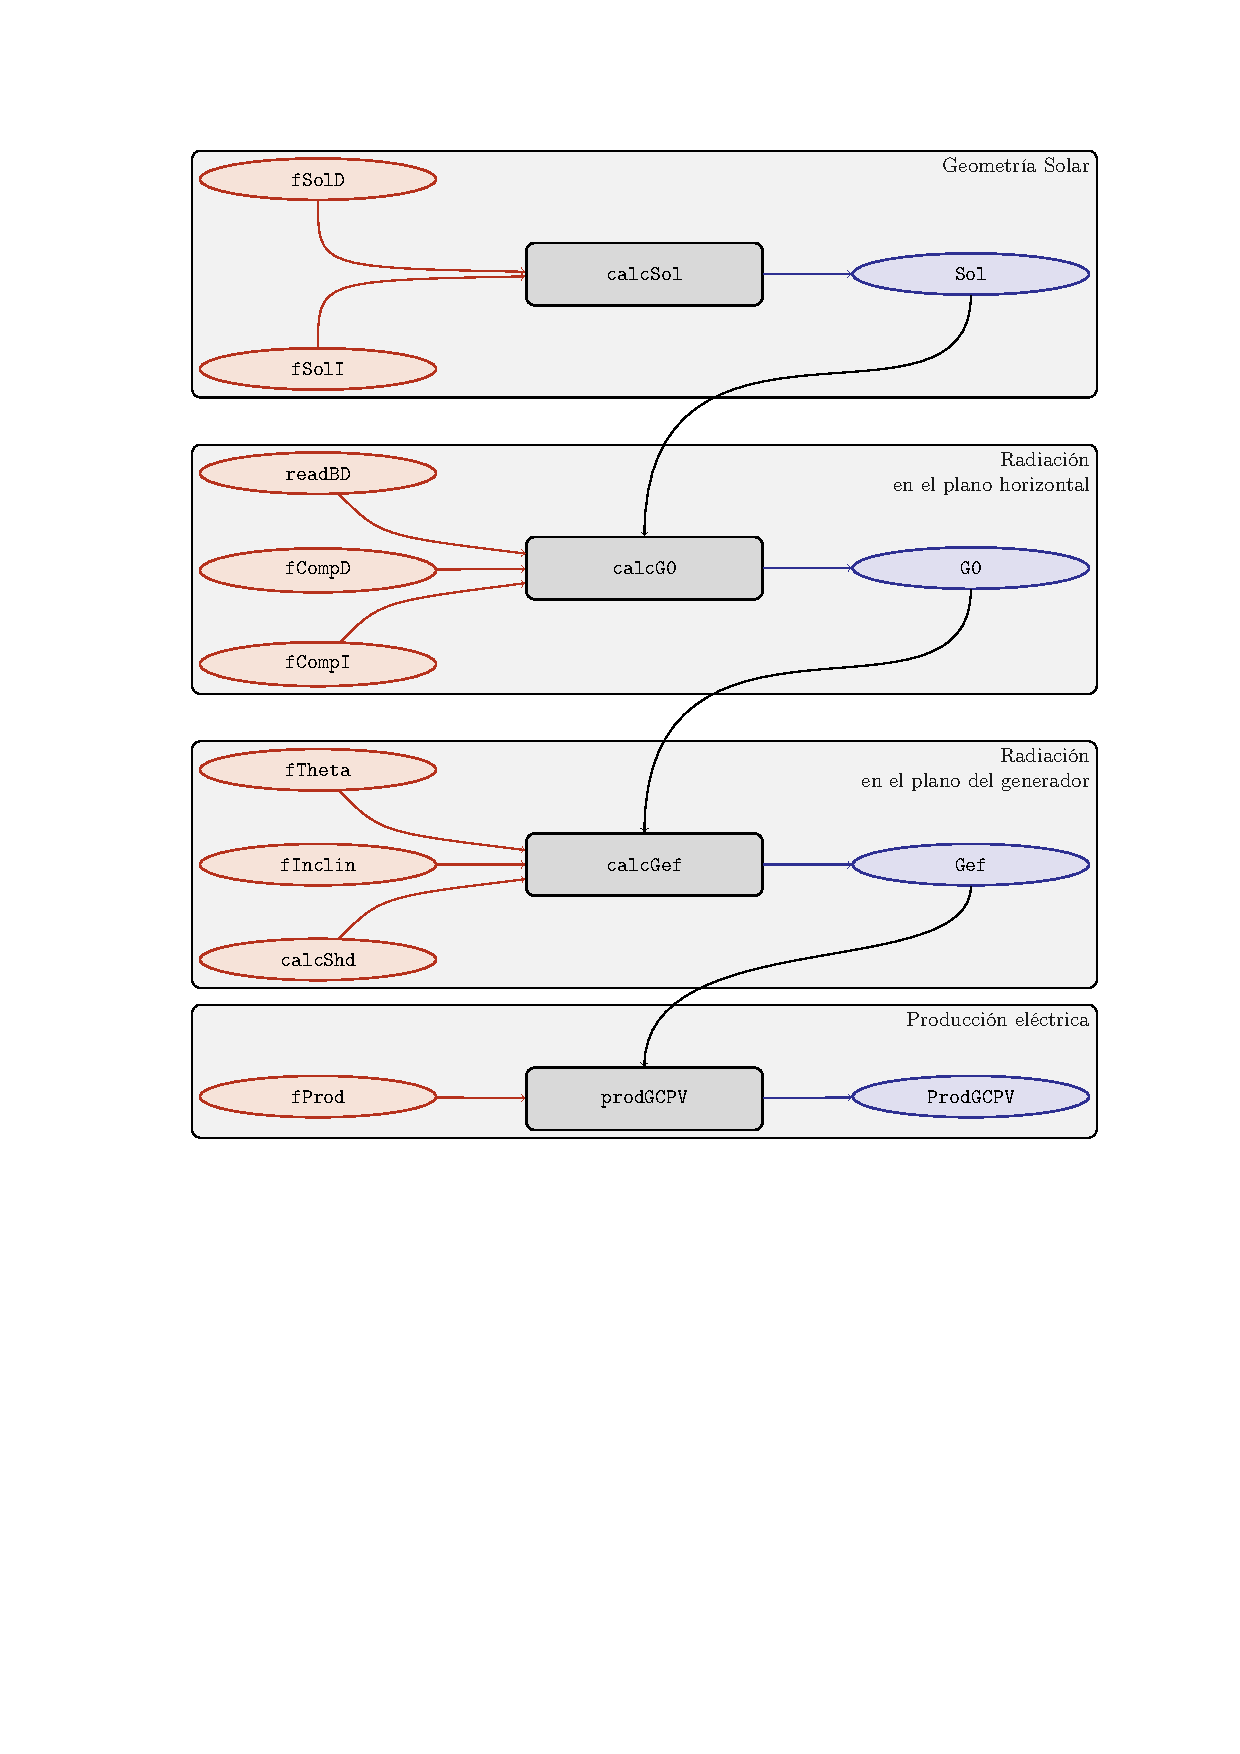
\includegraphics[keepaspectratio,width=0.8\textwidth,height=0.43\textheight]{figuras/procedure.pdf}
\caption{\label{fig:org25b93f6}Proceso de cálculo de las funciones de \texttt{solaR2}}
\end{figure}
A la hora de estimar la producción, el programa sigue los siguientes procesos\footnote{Todas las funciones recogidas en este capítulo, están descritas en el manual de uso del paquete \texttt{solaR2}, el cual, está disponible en el apendice \ref{chap:manual} de este documento.}:
\section{Geometría solar}
\label{sec:orgfbbab7c}
\label{sec:geometria-solar}
Para calcular la geometría que definen las posiciones de la Tierra y el Sol, \texttt{solaR2} se vale de una función constructora, \texttt{calcSol}, la cual mediante las funciones \texttt{fSolD} y \texttt{fSolI} cálcula todos los ángulos y componentes que caracterizan la geometría solar.
\begin{figure}[htbp]
\centering
\includegraphics[keepaspectratio,width=\textwidth,height=0.5\textheight]{figuras/calcSol.pdf}
\caption{Cálculo de la geometría solar mediante la función \texttt{calcSol}, la cual unifica las funciones \texttt{fSolD} y \texttt{fSolI} resultando en un objeto clase \texttt{Sol} el cual contiene toda la información geométrica necesaria para realizar las siguientes estimaciones. \label{fig:calcSol}}
\end{figure}

Como se puede ver en la figura \ref{fig:calcSol}, \texttt{calcSol} funcia gracias a las siguientes funciones:
\begin{itemize}
\item \texttt{fSolD}: la cual, a partir de la latitud (\(\phi\)), calcula la geometría a nivel diario, es decir, los ángulos y componentes que se pueden calcular en cada día independiente.
Estas son:
\begin{itemize}
\item Declinación (\(\delta\)): calculada a partir de la función \texttt{declination}.
\item Excentricidad (\(\epsilon_o\)): obtenida mediante la función \texttt{eccentricity}.
\item Ecuación del tiempo (\(EoT\)): obtenida mediante la función \texttt{eot}.
\item Ángulo del amanecer (\(\omega_s\)): calculada a partir de la función \texttt{sunrise}.
\item Irradiancia diaria extra-atmosférica (\(B_{0d}(0)\)): obtenida a paritr de la función \texttt{bo0d}.
\end{itemize}
\end{itemize}
\begin{lstlisting}[numbers=left,language=r,label= ,caption= ,captionpos=b]
lat <- 37.2
BTd <- fBTd(mode = 'prom')
solD <- fSolD(lat = lat, BTd = BTd)
show(solD)
\end{lstlisting}

\begin{verbatim}
Key: <Dates>
         Dates   lat        decl        eo           EoT        ws      Bo0d
        <IDat> <num>       <num>     <num>         <num>     <num>     <num>
 1: 2024-01-17  37.2 -0.36271754 1.0340422 -0.0455346238 -1.278593  4738.993
 2: 2024-02-14  37.2 -0.22850166 1.0259717 -0.0614793356 -1.393341  6137.388
 3: 2024-03-15  37.2 -0.03191616 1.0107943 -0.0368674274 -1.546560  8086.323
 4: 2024-04-15  37.2  0.17531794 0.9926547  0.0017482721 -1.705659  9921.357
 5: 2024-05-15  37.2  0.33246485 0.9775162  0.0143055938 -1.835976 11115.619
 6: 2024-06-10  37.2  0.40257826 0.9691480 -0.0007378952 -1.899934 11573.907
 7: 2024-07-18  37.2  0.36439367 0.9675489 -0.0263454380 -1.864521 11257.133
 8: 2024-08-18  37.2  0.22407398 0.9758022 -0.0111761118 -1.744657 10183.208
 9: 2024-09-18  37.2  0.02730595 0.9907919  0.0342189964 -1.591529  8508.642
10: 2024-10-19  37.2 -0.17900474 1.0088406  0.0689613044 -1.433019  6554.218
11: 2024-11-18  37.2 -0.33862399 1.0245012  0.0575423573 -1.300179  4951.750
12: 2024-12-13  37.2 -0.40478283 1.0328516  0.0158622941 -1.239567  4284.472
\end{verbatim}

Tiene los siguientes argumentos:
\begin{itemize}
\item \texttt{lat}: para introducir la latitud en grados.
\item \texttt{BTd}: para introducir la base temporal \textbf{diaria} sobre la que se harán los cálculos.
\item \texttt{method}: para elegir el método de cálculo. Se puede elegir entre: \texttt{michalsky}, \texttt{cooper}, \texttt{spencer} y \texttt{strous}
\begin{lstlisting}[numbers=left,language=r,label= ,caption= ,captionpos=b]
BTd <- fBTd(mode = 'prom')
solD_michalsky <- fSolD(lat, BTd, method = 'michalsky')
solD_michalsky[, group := 'michalsky']
solD_cooper <- fSolD(lat, BTd, method = 'cooper')
solD_cooper[, group := 'cooper']
solD_spencer <- fSolD(lat, BTd, method = 'spencer')
solD_spencer[, group := 'spencer']
solD_strous <- fSolD(lat, BTd, method = 'strous')
solD_strous[, group := 'strous']
solD_all <- rbind(solD_michalsky, solD_cooper,
                  solD_spencer, solD_strous)
xyplot(eo + ws + Bo0d ~ Dates , solD_all,
       groups = group, type = 'l', auto.key = TRUE,
       par.settings = solaR.theme, scales = list(y = 'free'),
       ylab = '', layout = c(1, 3))
\end{lstlisting}

\begin{center}
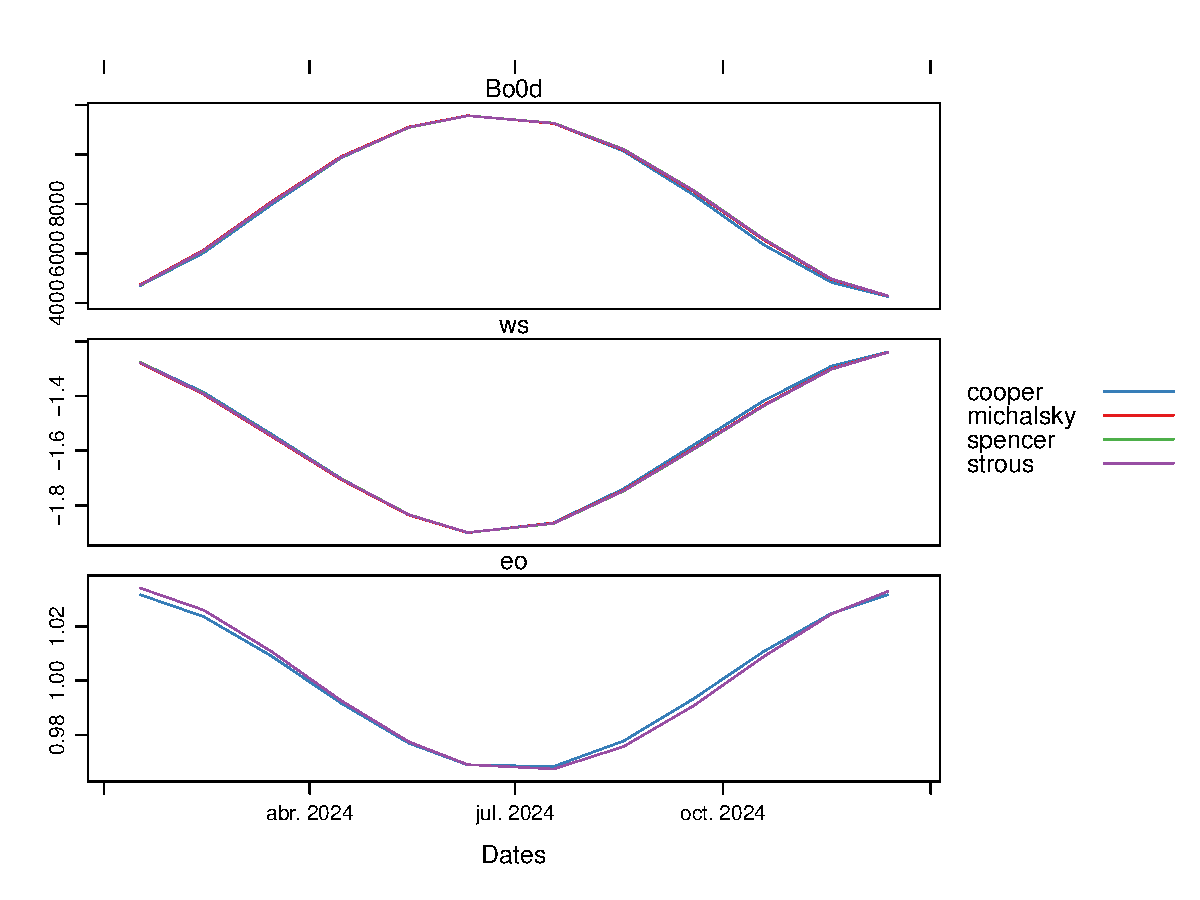
\includegraphics[width=0.8\textwidth]{figuras/codigo-fSolD.pdf}
\end{center}
\end{itemize}
\begin{itemize}
\item \texttt{fSolI}: toma los resultados obtenidos en \texttt{fSolD} y calcula la geometría a nivel intradiario, es decir, aquella que se puede calcular en unidades de tiempo menores a los días.
Estas son:
\begin{itemize}
\item La hora solar o tiempo solar verdadero (\(\omega\)): calculada a partir de la función \texttt{sunHour}.
\item Los momentos del día en los que es de noche (\(night\)): calculada a partir del resultado anterior y de el ángulo del amanecer (cálculada en \texttt{fSolD})\footnote{Cuando la hora solar verdadera excede los ángulos en los que amanece y anochece (\(|\omega|>=|\omega_s|\)), el Sol queda por debajo de la línea del horizonte, por lo que es de noche.}.
\item El coseno del ángulo cenital solar (\(cos(\theta_{zs})\)): obtenida a partir de la función \texttt{zenith}.
\item La altura solar (\(\gamma_s\)): obtenida a partir del resultado anterior\footnote{\(\gamma_s=asin(cos(\theta_s))\).}.
\item El ángulo acimutal solar (\(\theta_{zs}\)): calculada mediante la función \texttt{azimuth}.
\item La irradiancia extra-atmosférica (\(B_0(0)\)): calculada mediante el coseno del ángulo cenital, la constante solar (\(B_0\)) y la excentridad (cálculada en \texttt{fSolD}) [ecuación \ref{eq:irradianciaextra}].
\end{itemize}
Su argumento principal es \texttt{sample} con el cual se puede determinar el intervalo intradiario de cálculos.
\end{itemize}
\begin{lstlisting}[numbers=left,language=r,label= ,caption= ,captionpos=b]
solD <- solD[1] #Computo solo un día a fin mejorar la visualización
solI <- fSolI(solD = solD, sample = 'min') 
xyplot(solI)
\end{lstlisting}

\begin{center}
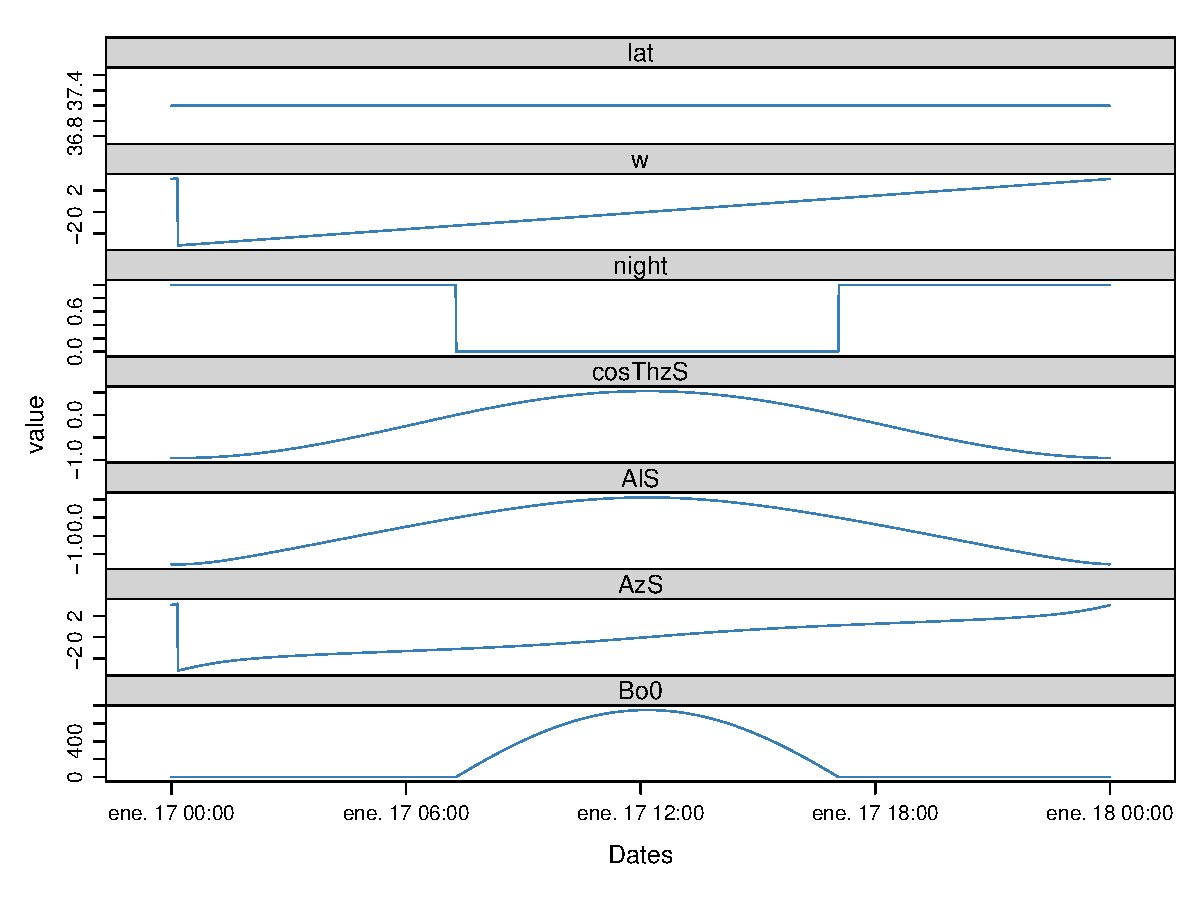
\includegraphics[width=0.8\textwidth]{figuras/codigo-solI.pdf}
\end{center}
  Además, como los datos nocturnos aportan poco a los cálculos que atañen a este proyecto, \texttt{fSolI} presenta la posibilidad de eliminar estos datos con el argumento \texttt{keep.night}.
\begin{lstlisting}[numbers=left,language=r,label= ,caption= ,captionpos=b]
solI_nigth <- fSolI(solD = solD, sample = 'min', keep.night = FALSE)
xyplot(solI_nigth)
\end{lstlisting}

\begin{center}
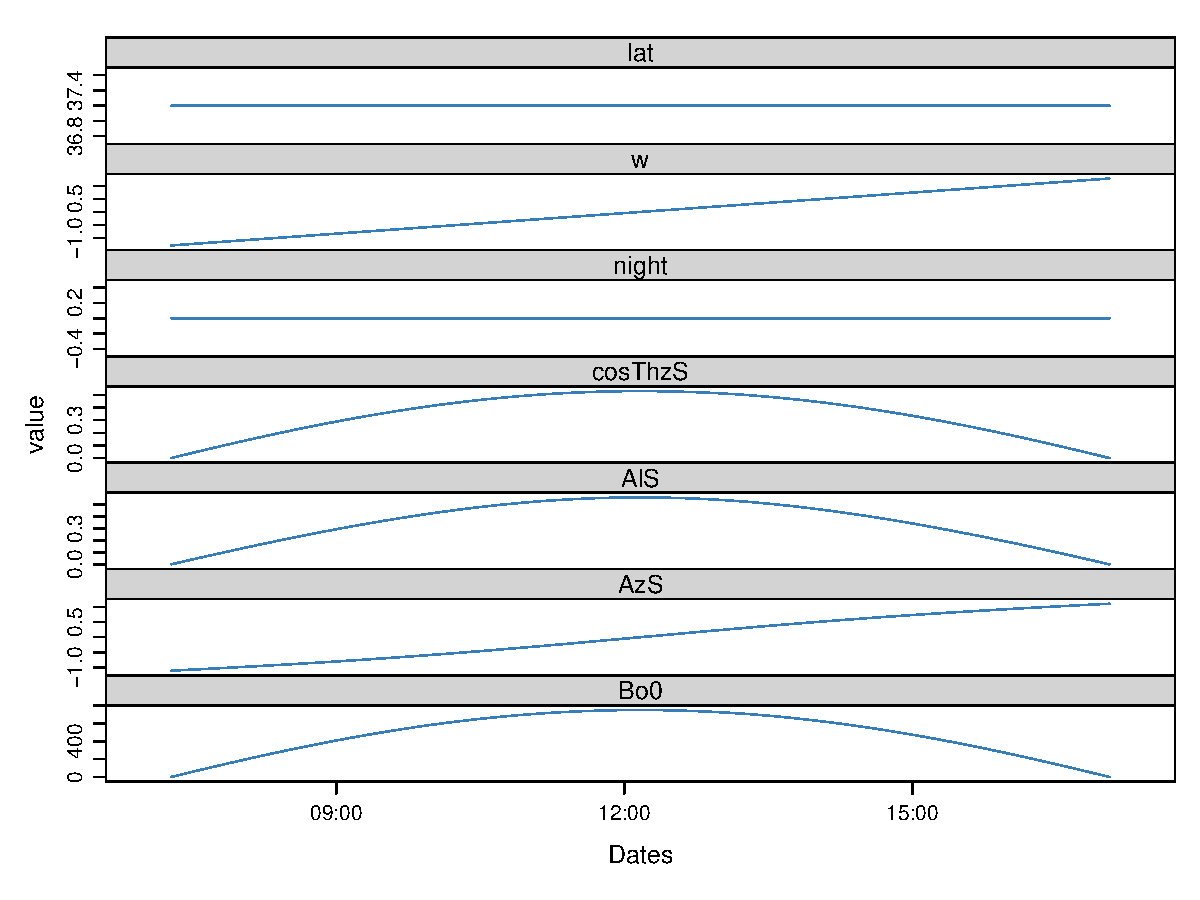
\includegraphics[width=0.8\textwidth]{figuras/codigo-solInight.pdf}
\end{center}
  Aparte, en vez de identificar el intervalo intradiario (con el argumento \texttt{sample}), se puede dar directamente la base temporal intradiaria.
\begin{lstlisting}[numbers=left,language=r,label= ,caption= ,captionpos=b]
BTd <- solD$Dates
BTi <- fBTi(BTd, sample = 'min')
solI_BTi <- fSolI(solD, BTi = BTi, keep.night = FALSE)
xyplot(solI_BTi)
\end{lstlisting}

\begin{center}
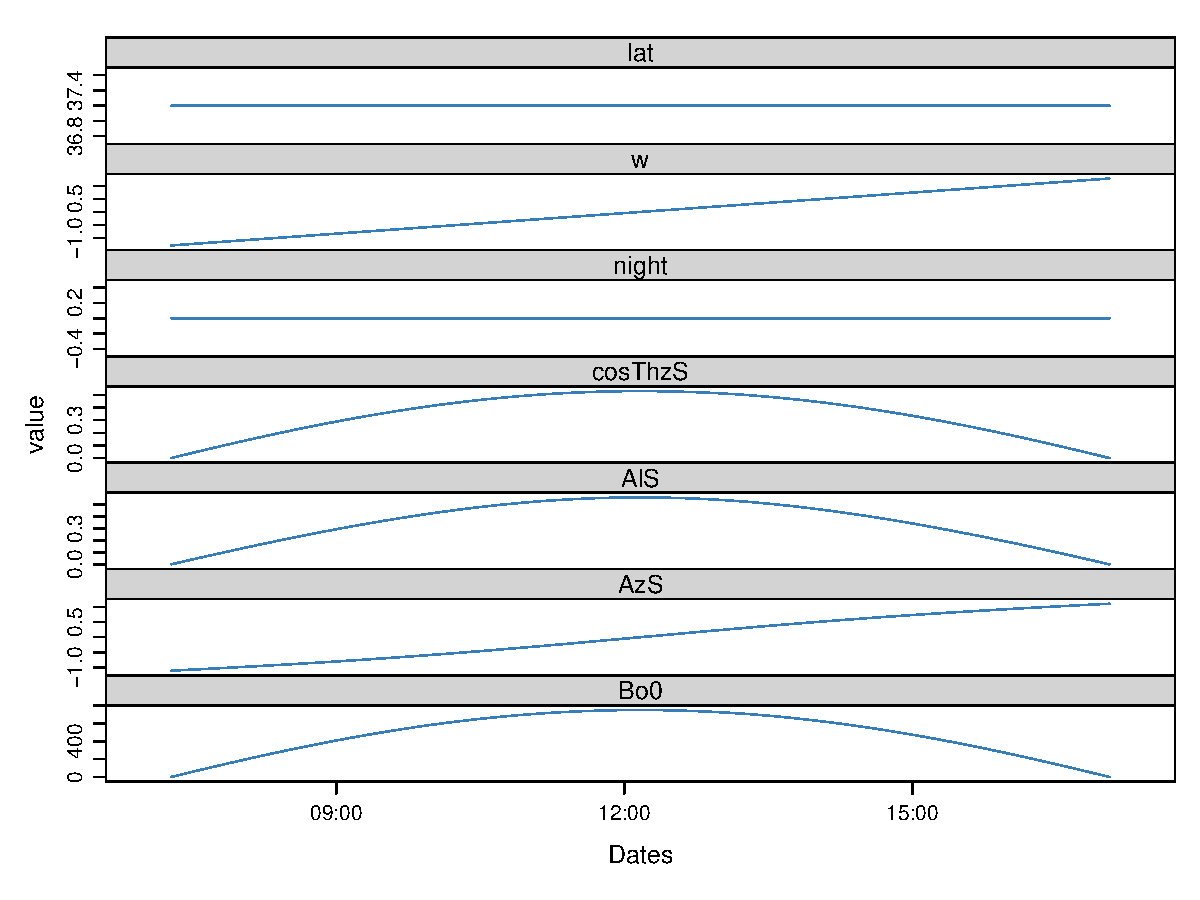
\includegraphics[width=0.8\textwidth]{figuras/codigo-solIBTi.pdf}
\end{center}
  También, se puede indicar que no realice las correcciones de la ecuación del tiempo.
\begin{lstlisting}[numbers=left,language=r,label= ,caption= ,captionpos=b]
solI_EoT <- fSolI(solD = solD, BTi = BTi, EoT = FALSE)
xyplot(solI_EoT)
\end{lstlisting}

\begin{center}
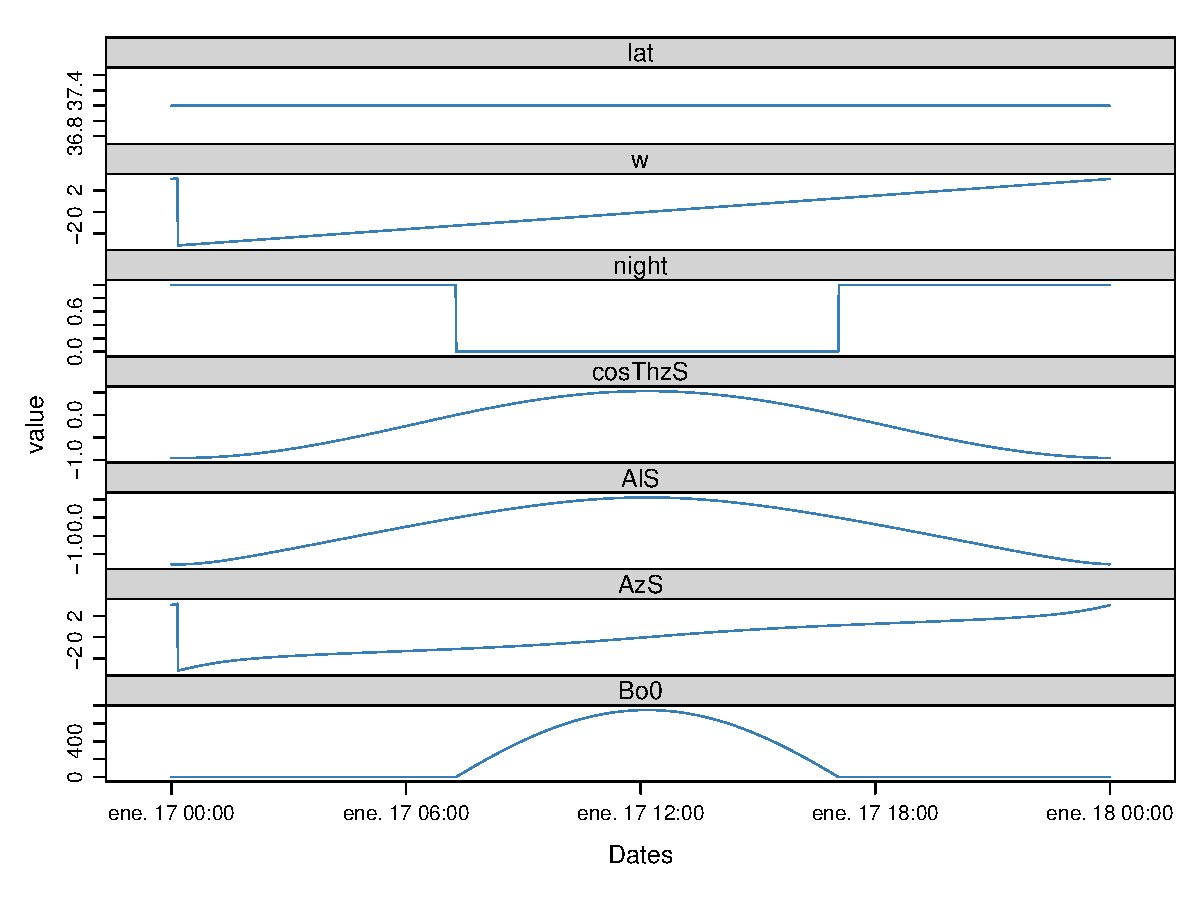
\includegraphics[width=0.8\textwidth]{figuras/codigo-solIEoT.pdf}
\end{center}

Finalmente, estas dos funciones, como se muestra en la figura \ref{fig:calcSol}, convergen en la función \texttt{calcSol}, dando como resultado un objeto de clase \texttt{Sol}. Este objeto muestra un resumen de ambos elementos junto con la latitud de los cálculos. Los argumentos de \texttt{calcSol} son las argumentos de las funciones anteriores
\begin{lstlisting}[numbers=left,language=r,label= ,caption= ,captionpos=b]
sol <- calcSol(lat = lat, BTd = BTd, sample = 'hour')
show(sol)
\end{lstlisting}

\begin{verbatim}
Object of class Sol 

Latitude:  37.2 degrees

Daily values:
     Dates                 decl               eo             EoT                 ws        
 Min.   :2024-01-17   Min.   :-0.3627   Min.   :1.034   Min.   :-0.04553   Min.   :-1.279  
 1st Qu.:2024-01-17   1st Qu.:-0.3627   1st Qu.:1.034   1st Qu.:-0.04553   1st Qu.:-1.279  
 Median :2024-01-17   Median :-0.3627   Median :1.034   Median :-0.04553   Median :-1.279  
 Mean   :2024-01-17   Mean   :-0.3627   Mean   :1.034   Mean   :-0.04553   Mean   :-1.279  
 3rd Qu.:2024-01-17   3rd Qu.:-0.3627   3rd Qu.:1.034   3rd Qu.:-0.04553   3rd Qu.:-1.279  
 Max.   :2024-01-17   Max.   :-0.3627   Max.   :1.034   Max.   :-0.04553   Max.   :-1.279  
      Bo0d     
 Min.   :4739  
 1st Qu.:4739  
 Median :4739  
 Mean   :4739  
 3rd Qu.:4739  
 Max.   :4739  

Intradaily values: 
     Dates                           w              night            cosThzS             AlS         
 Min.   :2024-01-17 00:00:00   Min.   :-2.92240   Mode :logical   Min.   :-0.9586   Min.   :-1.2819  
 1st Qu.:2024-01-17 05:45:00   1st Qu.:-1.41740   FALSE:10        1st Qu.:-0.7289   1st Qu.:-0.8172  
 Median :2024-01-17 11:30:00   Median : 0.08759   TRUE :14        Median :-0.2143   Median :-0.2160  
 Mean   :2024-01-17 11:30:00   Mean   : 0.08766                   Mean   :-0.2144   Mean   :-0.2724  
 3rd Qu.:2024-01-17 17:15:00   3rd Qu.: 1.59259                   3rd Qu.: 0.3003   3rd Qu.: 0.3051  
 Max.   :2024-01-17 23:00:00   Max.   : 3.09905                   Max.   : 0.5295   Max.   : 0.5580  
      AzS                Bo0       
 Min.   :-2.49463   Min.   :  0.0  
 1st Qu.:-1.18986   1st Qu.:  0.0  
 Median : 0.09526   Median :  0.0  
 Mean   : 0.08773   Mean   :197.0  
 3rd Qu.: 1.28896   3rd Qu.:424.5  
 Max.   : 3.00158   Max.   :748.4
\end{verbatim}


\section{Datos meteorológicos}
\label{sec:orgb95d316}
\label{sec:datos-meteorologicos}
Para el procesamiento de datos meteorologicos, \texttt{solaR2} provee una serie de funciones que son capaces de leer todo tipo de datos. Estos datos se procesan y se almacenan en un objeto de tipo \texttt{Meteo} tal y como se ve en la figura \ref{fig:meteo}. Estas funciones son:
\begin{figure}[htbp]
\centering
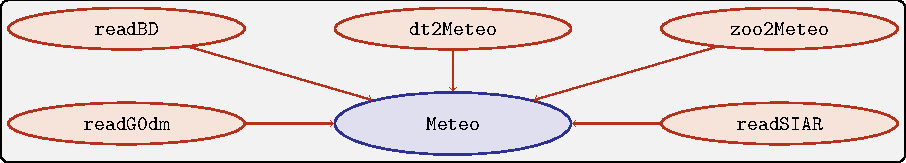
\includegraphics[keepaspectratio,width=\textwidth,height=0.5\textheight]{figuras/meteo.pdf}
\caption{Los datos meteorologicas se pueden leer mediante las funciones \texttt{readG0dm}, \texttt{readBD}, \texttt{dt2Meteo}, \texttt{zoo2Meteo} y \texttt{readSIAR} las cuales procesan estos datos y los almacenan en un objeto de clase \texttt{Meteo}. \label{fig:meteo}}
\end{figure}
\begin{itemize}
\item \texttt{readG0dm}: Esta función construye un objeto \texttt{Meteo} a partir de 12 valores de medias mensuales de irradiación.
Como argumentos tiene:
\begin{itemize}
\item \texttt{G0dm}: vector con medias mensuales de irradiación global horizontal.
\item \texttt{Ta}: vector con la temperatura ambiente.
\item \texttt{lat}: latitud en grados.
\item \texttt{year}: año de los datos. Por defecto presenta el año actual.
\item \texttt{source}: información de la fuente de los datos.
\end{itemize}
\end{itemize}
\begin{lstlisting}[numbers=left,language=r,label= ,caption= ,captionpos=b]
G0dm = c(2.766,3.491,4.494,5.912,6.989,7.742,
         7.919,7.027,5.369,3.562,2.814,2.179) * 1000;
Ta = c(10, 14.1, 15.6, 17.2, 19.3, 21.2,
       28.4, 29.9, 24.3, 18.2, 17.2, 15.2)
BD <- readG0dm(G0dm = G0dm, Ta = Ta, lat = 37.2)
xyplot(BD)
\end{lstlisting}

\begin{center}
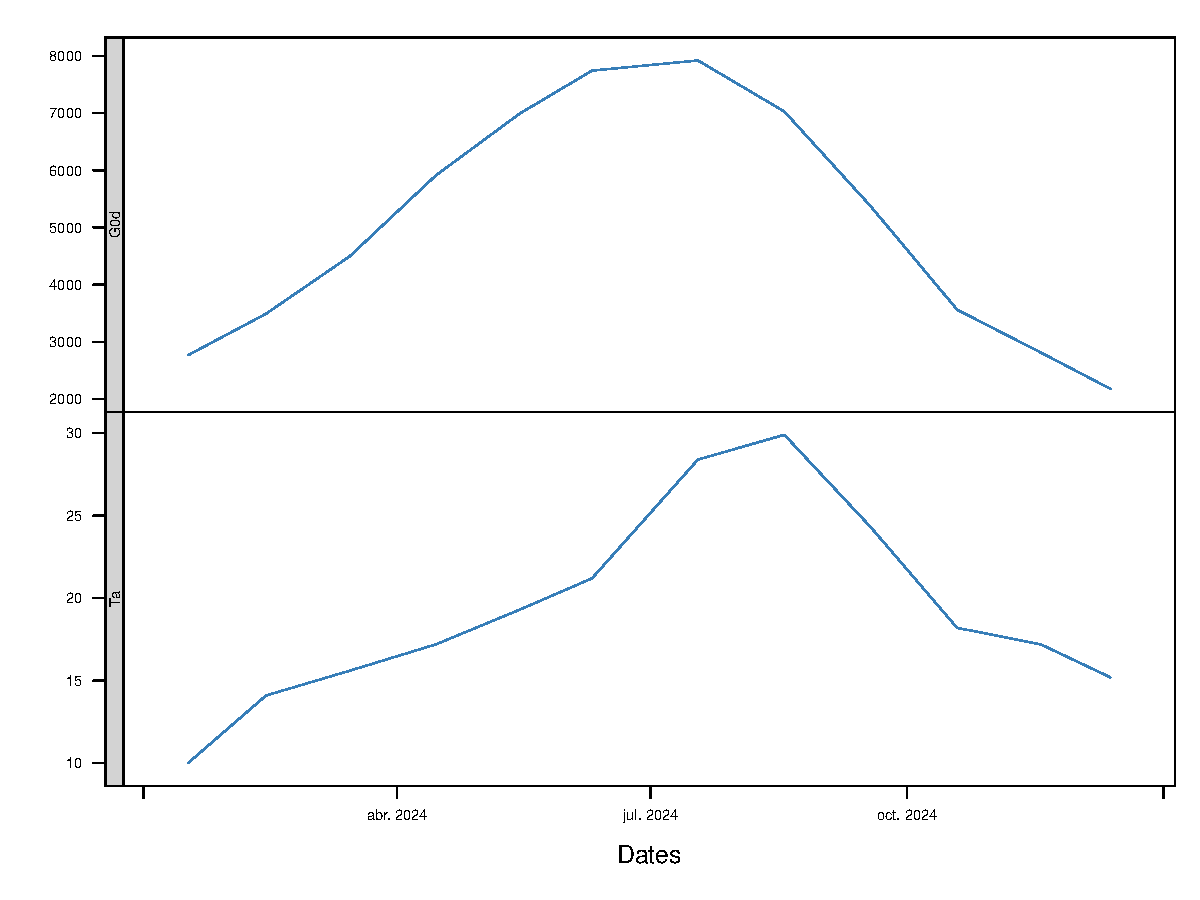
\includegraphics[width=0.8\textwidth]{figuras/codigo-readg0dm.pdf}
\end{center}
\begin{itemize}
\item \texttt{readBD}: Esta familia de funciones puede leer ficheros de datos y transformarlos en un objeto de clase \texttt{Meteo}. Se dividen en:
\begin{itemize}
\item \texttt{readBDd}: Procesa datos meteorológicos de tipo diarios.
Como argumentos tiene:
\begin{itemize}
\item \texttt{file}: nombre del archivo que contiene los datos.
\item \texttt{lat}: latitud en grados.
\item \texttt{format}: formato de los datos de fechas.
\item \texttt{header}, \texttt{fill}, \texttt{dec}, \texttt{sep}: argumentos para \href{https://search.r-project.org/CRAN/refmans/data.table/html/fread.html}{\texttt{fread}}.
\item \texttt{dates.col}: nombre de la columna que contiene los datos de fechas. Por defecto es 'Dates'.
\item \texttt{ta.col}: nombre de la columna que contiene los datos de temperatura. Por defecto es 'Ta'.
\item \texttt{g0.col}: nombre de la columna que contiene los datos de irradiación. Por defecto es 'G0'.
\item \texttt{keep.cols}: si su valor es \texttt{TRUE}, mantiene las columnas que no sean importantes para el resto de operaciones.
\end{itemize}
\end{itemize}
\begin{lstlisting}[numbers=left,language=r,label= ,caption= ,captionpos=b]
## Se utiliza un archivo alojado en el
## github del tutor de este proyecto 
myURL <-"https://raw.githubusercontent.com/oscarperpinan/R/master/data/aranjuez.csv"
download.file(myURL, 'data/aranjuez.csv', quiet = TRUE)
BDd <- readBDd(file = 'data/aranjuez.csv', lat = lat,
               format = '%Y-%m-%d', header = TRUE,
               fill = TRUE, dec = '.', sep = ',', dates.col = '',
               ta.col = 'TempAvg', g0.col = 'Radiation', keep.cols = TRUE)
xyplot(BDd)
\end{lstlisting}

\begin{center}
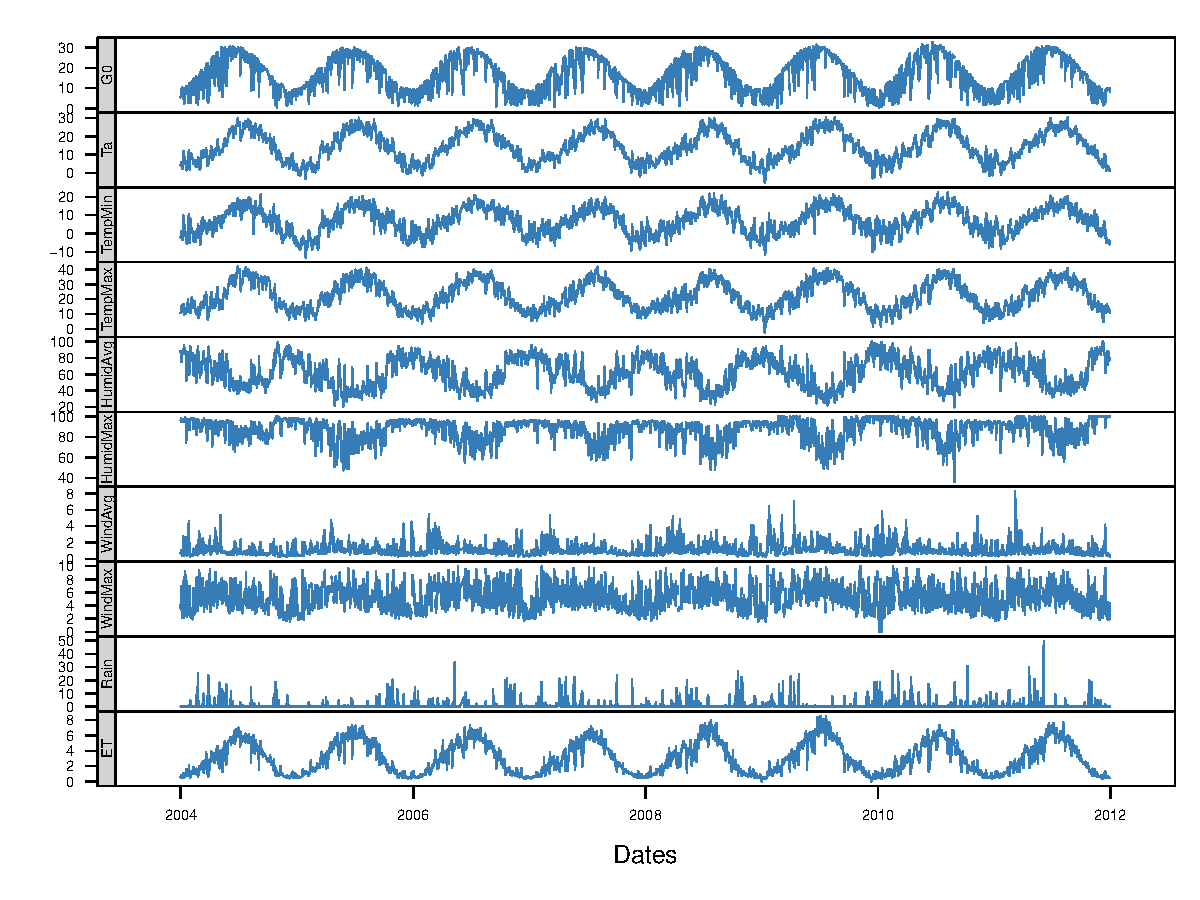
\includegraphics[width=0.8\textwidth]{figuras/codigo-readBD.pdf}
\end{center}
\begin{itemize}
\item \texttt{readBDi}: Procesa datos meteorológicos de tipo intradiarios.
Como argumentos tiene:
\begin{itemize}
\item \texttt{file}: nombre del archivo que contiene los datos.
\item \texttt{lat}: latitud en grados.
\item \texttt{format}: formato de los datos de fechas.
\item \texttt{header}, \texttt{fill}, \texttt{dec}, \texttt{sep}: argumentos para \href{https://search.r-project.org/CRAN/refmans/data.table/html/fread.html}{\texttt{fread}}.
\item \texttt{dates.col}: nombre de la columna que contiene los datos de fechas y/o tiempos. Por defecto es 'Dates'.
\item \texttt{times.col}: nombre de la columna que contiene los datos de tiempos en caso de que \texttt{dates.col} no los incluyera.
\item \texttt{ta.col}: nombre de la columna que contiene los datos de temperatura. Por defecto es 'Ta'.
\item \texttt{g0.col}: nombre de la columna que contiene los datos de irradiancia. Por defecto es 'G0'.
\item \texttt{keep.cols}: si su valor es \texttt{TRUE}, mantiene las columnas que no sean importantes para el resto de operaciones.
\end{itemize}
\end{itemize}
\begin{lstlisting}[numbers=left,language=r,label= ,caption= ,captionpos=b]
myURL <- "https://raw.githubusercontent.com/oscarperpinan/R/master/data/NREL-Hawaii.csv"
download.file(myURL, 'data/NREL-Hawaii.csv', quiet = TRUE)
BDi <- readBDi(file = 'data/NREL-Hawaii.csv', lat = 19,
               format = "%d/%m/%Y %H:%M", header = TRUE,
               fill = TRUE, dec = '.', sep = ',',
               dates.col = 'DATE', times.col = 'HST',
               ta.col = 'Air Temperature [deg C]',
               g0.col = 'Global Horizontal [W/m^2]',
               keep.cols = TRUE)
xyplot(BDi)
\end{lstlisting}

\begin{center}
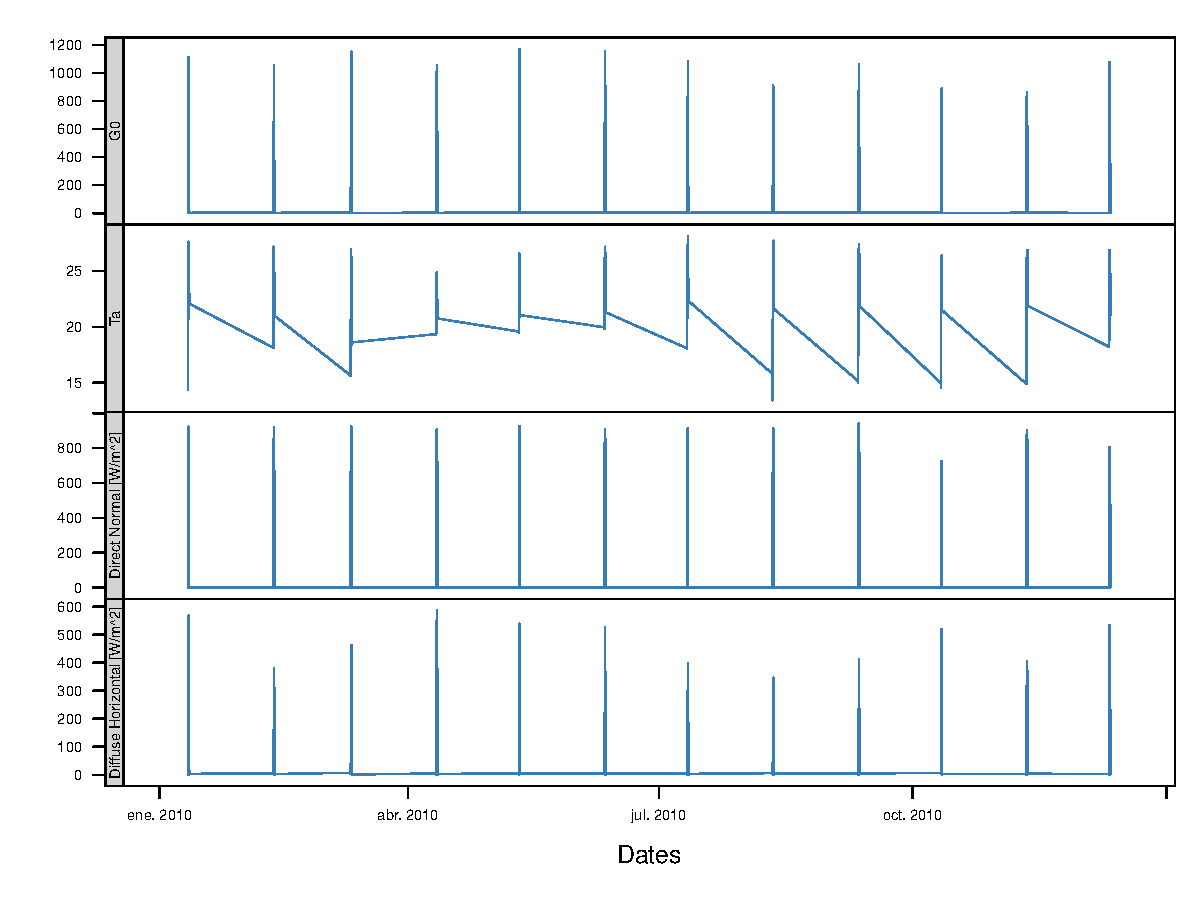
\includegraphics[width=0.8\textwidth]{figuras/codigo-readBDi.pdf}
\end{center}
\item \texttt{dt2Meteo}: Transforma un \texttt{data.table} o \texttt{data.frame} en un objeto de clase \texttt{Meteo}.
Como argumentos tiene:
\begin{itemize}
\item \texttt{file}: \texttt{data.table} que contiene los datos.
\item \texttt{lat}: latitud en grados.
\item \texttt{source}: información sobre la fuente de los datos.
\item \texttt{type}: tipo de datos. A elegir  entre \texttt{bdI} (intradiarios), \texttt{bd} (diarios) y \texttt{prom} (medias mensuales). Si no viene dado, lo calcula por su cuenta.
\end{itemize}
\end{itemize}
\begin{lstlisting}[numbers=left,language=r,label= ,caption= ,captionpos=b]
data(helios)
names(helios) <- c('Dates', 'G0d', 'TempMax', 'TempMin')
helios_meteo <- dt2Meteo(file = helios, lat = 40, type = 'bd')
xyplot(helios_meteo)
\end{lstlisting}

\begin{center}
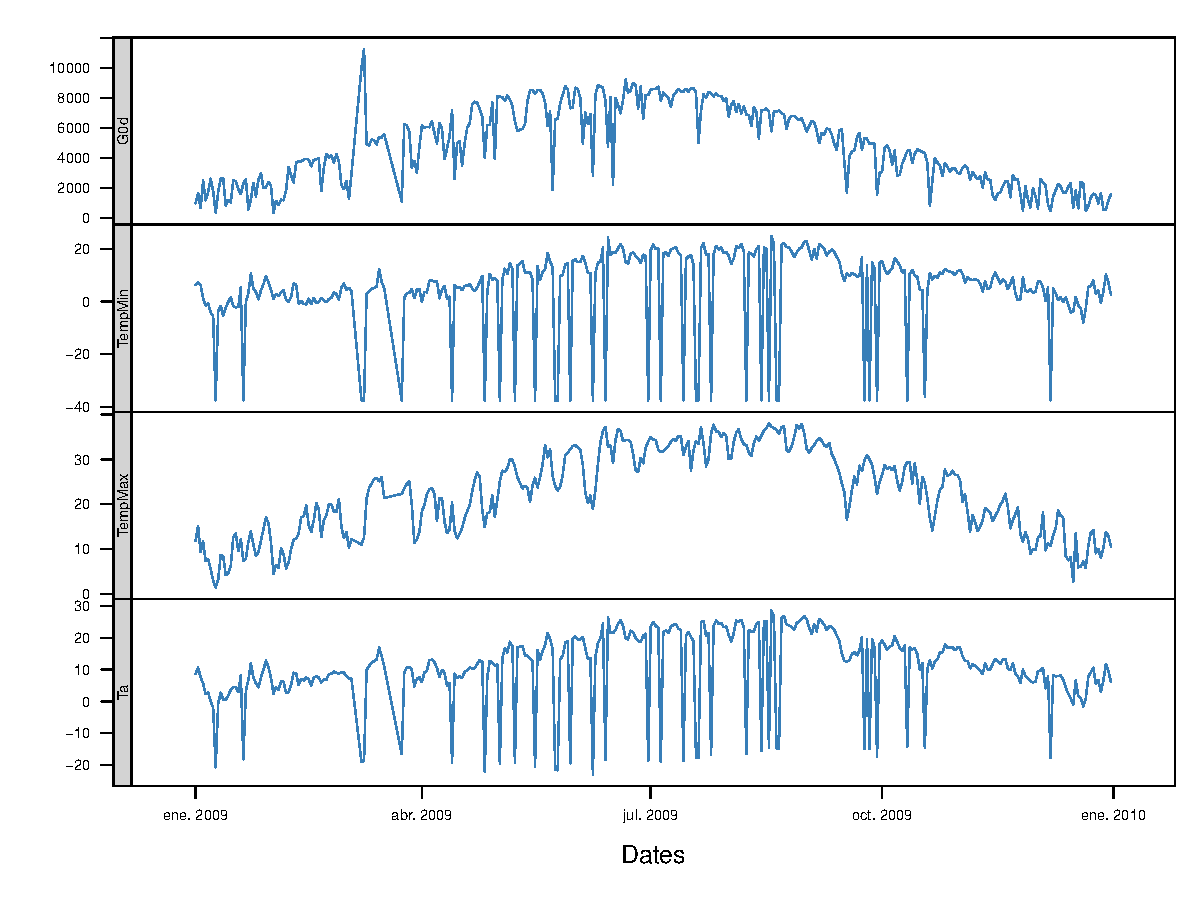
\includegraphics[width=0.8\textwidth]{figuras/codigo-dt2meteo.pdf}
\end{center}
\begin{itemize}
\item \texttt{zoo2Meteo}: Transforma un objeto de clase \texttt{zoo}\footnote{Pese a que este proyecto trate de ``desligarse'' del paquete \texttt{zoo}, sigue siendo un paquete muy extendido. Por lo que es interesante tener una función así para que los usuarios tengan una mayor flexibilidad.} en un objeto de clase \texttt{Meteo}.
Como argumentos tiene:
\begin{itemize}
\item \texttt{file}: \texttt{data.table} que contiene los datos.
\item \texttt{lat}: latitud en grados.
\item \texttt{source}: información sobre la fuente de los datos.
\end{itemize}
\end{itemize}
\begin{lstlisting}[numbers=left,language=r,label= ,caption= ,captionpos=b]
library(zoo)
bd_zoo <- read.csv.zoo('data/aranjuez.csv')
BD_zoo <- zoo2Meteo(file = bd_zoo, lat = 40)
show(BD_zoo)
\end{lstlisting}

\begin{verbatim}
Object of class  Meteo 

Source of meteorological information: bd-zoo-bd_zoo 
Latitude of source:  40 degrees

Meteorological Data:
    TempAvg          TempMax          TempMin           HumidAvg         HumidMax         WindAvg     
 Min.   :-5.309   Min.   :-2.362   Min.   :-12.980   Min.   : 19.89   Min.   : 35.88   Min.   :0.251  
 1st Qu.: 7.692   1st Qu.:14.530   1st Qu.:  1.515   1st Qu.: 47.04   1st Qu.: 81.60   1st Qu.:0.667  
 Median :13.810   Median :21.670   Median :  7.170   Median : 62.58   Median : 90.90   Median :0.920  
 Mean   :14.405   Mean   :22.531   Mean   :  6.888   Mean   : 62.16   Mean   : 87.22   Mean   :1.174  
 3rd Qu.:21.615   3rd Qu.:30.875   3rd Qu.: 12.590   3rd Qu.: 77.38   3rd Qu.: 94.90   3rd Qu.:1.431  
 Max.   :30.680   Max.   :41.910   Max.   : 22.710   Max.   :100.00   Max.   :100.00   Max.   :8.260  
                                   NA's   :4                          NA's   :13       NA's   :8      
    WindMax            Rain          Radiation            ET       
 Min.   : 0.000   Min.   : 0.000   Min.   : 0.277   Min.   :0.000  
 1st Qu.: 3.783   1st Qu.: 0.000   1st Qu.: 9.370   1st Qu.:1.168  
 Median : 5.027   Median : 0.000   Median :16.660   Median :2.758  
 Mean   : 5.208   Mean   : 1.094   Mean   :16.742   Mean   :3.091  
 3rd Qu.: 6.537   3rd Qu.: 0.200   3rd Qu.:24.650   3rd Qu.:4.926  
 Max.   :10.000   Max.   :49.730   Max.   :32.740   Max.   :8.564  
 NA's   :128      NA's   :4        NA's   :13       NA's   :18
\end{verbatim}

\begin{itemize}
\item \texttt{readSIAR}: Esta función es capaz de extraer información de la red SIAR\footnote{La red SiAR (Sistema de Información Agroclimática para el Regadio) es una infraestructura que captura, registra y divulga los datos climáticos necesarios para el cálculo de la demanda hídrica en las zonas de riego \cite{siar23}.} y transformarlo en un objeto de clase \texttt{Meteo}.
Como argumentos tiene:
\begin{itemize}
\item \texttt{Lon}: Longitud en grados.
\item \texttt{Lat}: Latitud en grados.
\item \texttt{inicio}: Primer día de los registros.
\item \texttt{final}: Último día de los registros.
\item \texttt{tipo}: La API SIAR\footnote{La API (Interfaz de Programación de Aplicaciones) que se usa para la función \texttt{readSIAR} está proporcionada por la propia red SIAR \cite{siar23}.} permite tener 4 tipos de registros: \texttt{Mensuales}, \texttt{Semanales}, \texttt{Diarios} y \texttt{Horarios}.
\item \texttt{n\_est}: Con este argumento, la función es capaz de localizar el número seleccionado de estaciones más proximas a la ubicación dada, y obtener los datos individuales de cada una de ellas. Una vez obtenidos estos datos realiza una interpolación de distancia inversa ponderada (IDW\footnote{La interpolación IDW es un método de interpolación que estima el valor de un punto desconocido basado en los valores conocidos de puntos cercanos. Los puntos más cercanos tienen más peso en la estimación que los más lejanos, utilizando una relación inversa con la distancia.}) y entrega un solo resultado. Es importante añadir que la API SIAR tiene una limitación a la solicitud de registros que se le hace cada minuto, por lo que esta función cuenta con un comprobante para impedir que el usuario exceda este límite.
\end{itemize}
\end{itemize}
\begin{lstlisting}[numbers=left,language=r,label= ,caption= ,captionpos=b]
library(httr2)
library(jsonlite)
bd_SIAR <- readSIAR(Lat = 40.40596822621351, Lon = -3.70038308516172,
                    ## Ubicación de la Escuela Técnica Superior
                    ## de Ingeniería y Diseño Industrial (ETSIDI)
                    inicio = '2023-09-01', final = '2024-08-01',
                    tipo = 'Mensuales', n_est = 3)
xyplot(bd_SIAR)
\end{lstlisting}

\begin{center}
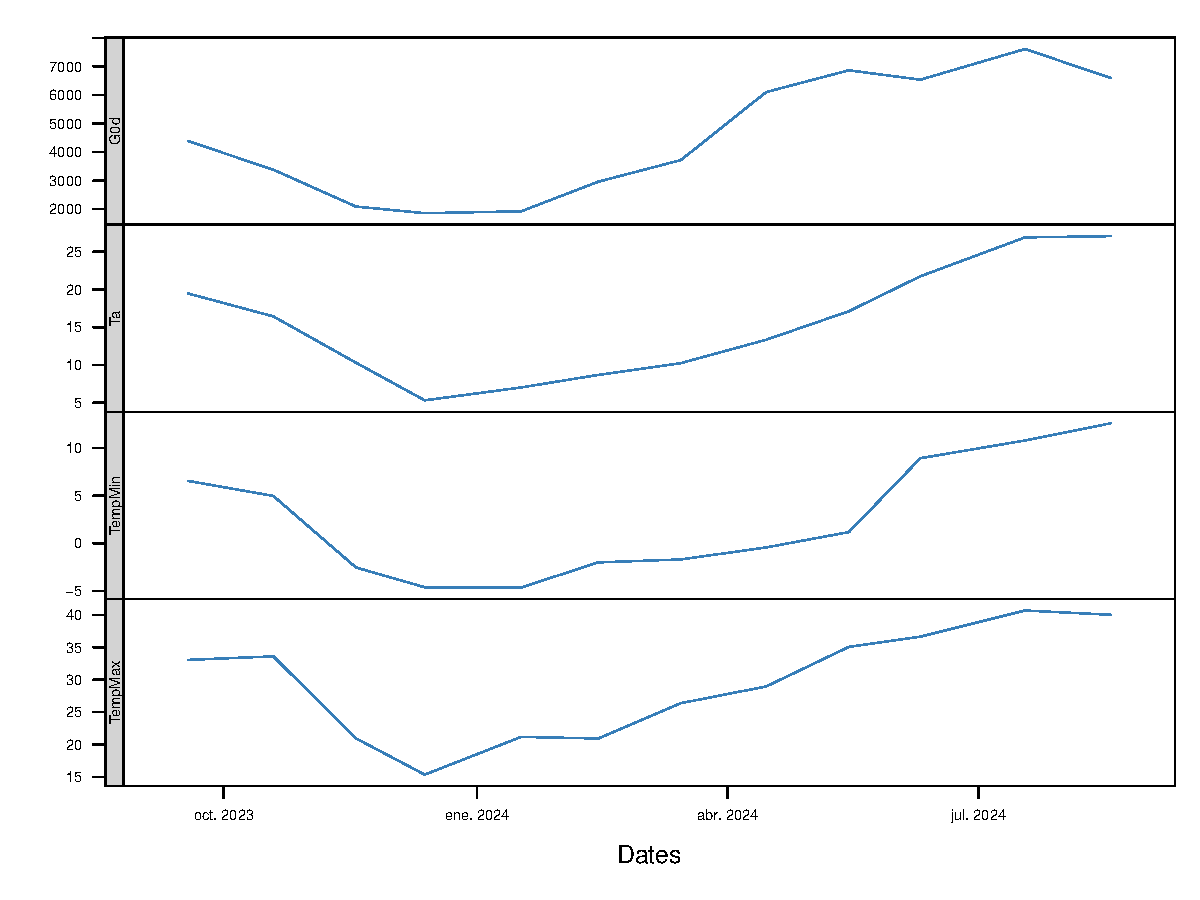
\includegraphics[width=0.8\textwidth]{figuras/codigo-readsiar.pdf}
\end{center}

\section{Radiación en el plano horizontal}
\label{sec:org3d1d929}
\label{sec:radiacion-plano-horizontal}
Una vez se ha calculado la geometría solar (sección \ref{sec:geometria-solar}) y se han procesado los datos meteorológicos (sección \ref{sec:datos-meteorologicos}), es necesario calcular la radiación en el plano horizontal. Para ello, \texttt{solaR2} cuenta con la función \texttt{calcG0} la cual mediante las funciones \texttt{fCompD} y \texttt{fCompI} procesan los objetos de clase \texttt{Sol} y clase \texttt{Meteo} para dar un objeto de tipo \texttt{G0}.

Como se puede ver en la figura \ref{fig:calcg0}, \texttt{calcG0} funciona gracias a las siguientes funciones:
\begin{figure}[htbp]
\centering
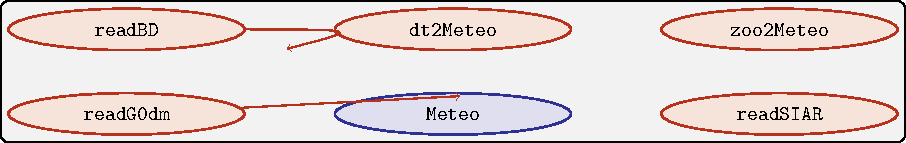
\includegraphics[keepaspectratio,width=\textwidth,height=0.5\textheight]{figuras/calcg0.pdf}
\caption{Cálculo de la radiación incidente en el plano horizontal mediante la función \texttt{calcG0}, la cual procesa un objeto clase \texttt{Sol} y otro clase \texttt{Meteo} mediante las funciones \texttt{fCompD} y \texttt{fCompI} resultando en un objeto clase \texttt{G0}. :\label{fig:calcg0}}
\end{figure}
\begin{itemize}
\item \texttt{fCompD}: La cual calcula todas las componentes de la irradiación diaria en una superficie horizontal mediante regresiones entre los parámetros del índice de claridad y la fracción difusa.
Tiene los siguientes argumentos:
\begin{itemize}
\item \texttt{sol}: Un objeto de clase \texttt{Sol}.
\item \texttt{G0d}: Un objeto clase \texttt{Meteo} o un \texttt{data.table} con datos de irradiación diaria en una superficie horizontal.
\item \texttt{corr}: A elegir el tipo de correlación entre la fracción de difusa y el índice de claridad.
Dependiendo del tipo de datos:
\begin{itemize}
\item Mensuales:
\end{itemize}
\begin{lstlisting}[numbers=left,language=r,label= ,caption= ,captionpos=b]
lat <- 37.2
BTd <- fBTd(mode = 'prom')
solD <- fSolD(lat, BTd)
G0d <- c(2.766,3.491,4.494,5.912,6.989,7.742,7.919,7.027,5.369,3.562,2.814,2.179) * 1000
compD_page <- fCompD(sol = solD, G0d = G0d, corr = "Page")
compD_page[, group := 'page']
compD_lj <- fCompD(sol = solD, G0d = G0d, corr = "LJ")
compD_lj[, group := 'lj']
compD_dia <- rbind(compD_page, compD_lj)
xyplot(Fd + D0d + B0d ~ Dates, compD_dia,
       groups = group, type = 'l', auto.key = TRUE,
       par.settings = solaR.theme, scales = list(y = 'free'),
       ylab = '', layout = c(1, 3))

\end{lstlisting}

\begin{center}
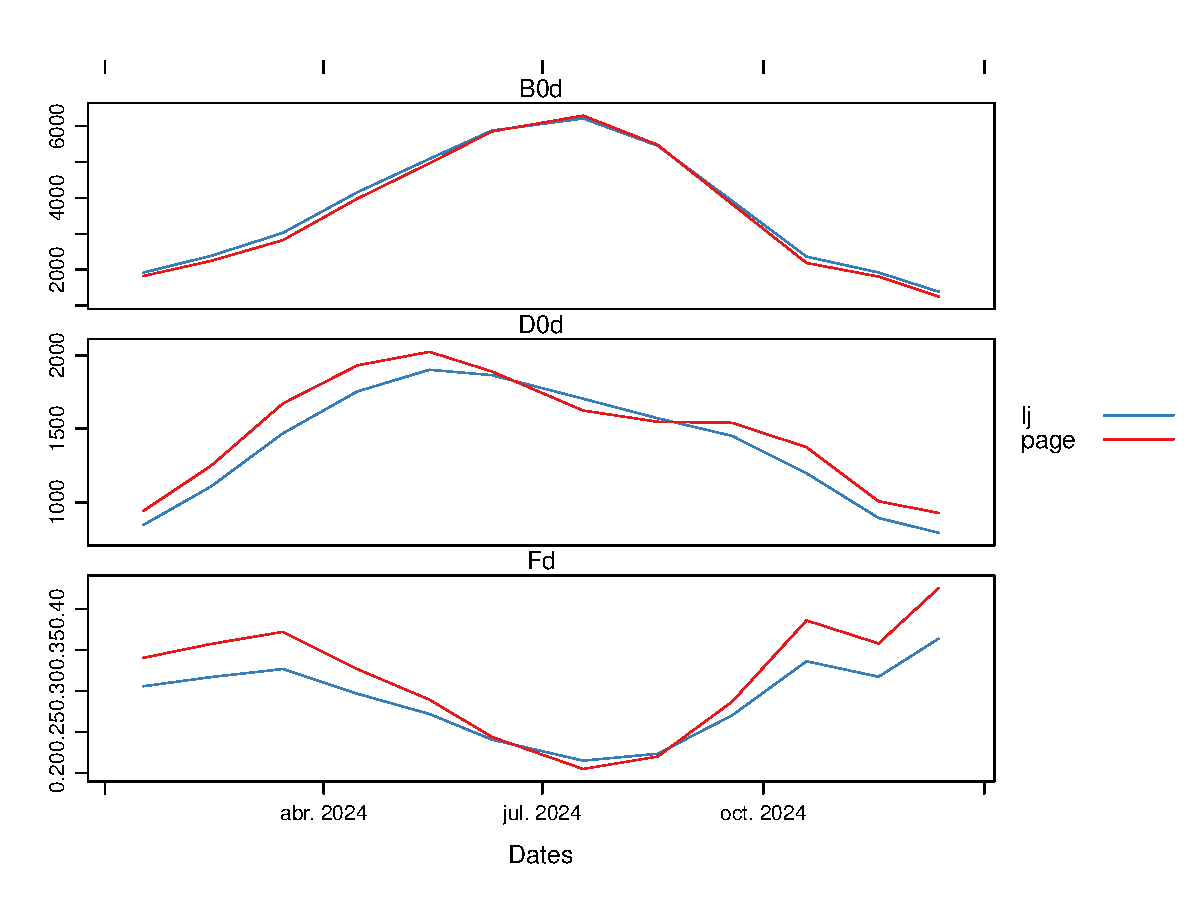
\includegraphics[width=0.8\textwidth]{figuras/codigo-fcompdmes.pdf}
\end{center}
\begin{itemize}
\item Diarios:
\end{itemize}
\begin{lstlisting}[numbers=left,language=r,label= ,caption= ,captionpos=b]
G0d <- readSIAR(Lat = 40.40596822621351, Lon =-3.70038308516172,
                inicio = '2024-07-15', final = '2024-08-01',
                tipo = 'Diarios', n_est = 3)
sol <- calcSol(lat, BTd = indexD(G0d))
compD_cpr <- fCompD(sol = sol, G0d = G0d, corr = "CPR")
compD_cpr[, group := 'cpr']
compD_ekdd <- fCompD(sol = sol, G0d = G0d, corr = 'EKDd')
compD_ekdd[, group := 'ekdd']
compD_climedd <- fCompD(sol = sol, G0d = G0d, corr = 'CLIMEDd')
compD_climedd[, group := 'climedd']
compD_mes <- rbind(compD_cpr, compD_ekdd, compD_climedd)
xyplot(Fd + D0d + B0d ~ Dates, compD_mes,
       groups = group, type = 'l',auto.key = TRUE,
       par.settings = solaR.theme, scales = list(y = 'free'),
       ylab = '', layout = c(1, 3))
\end{lstlisting}

\begin{center}
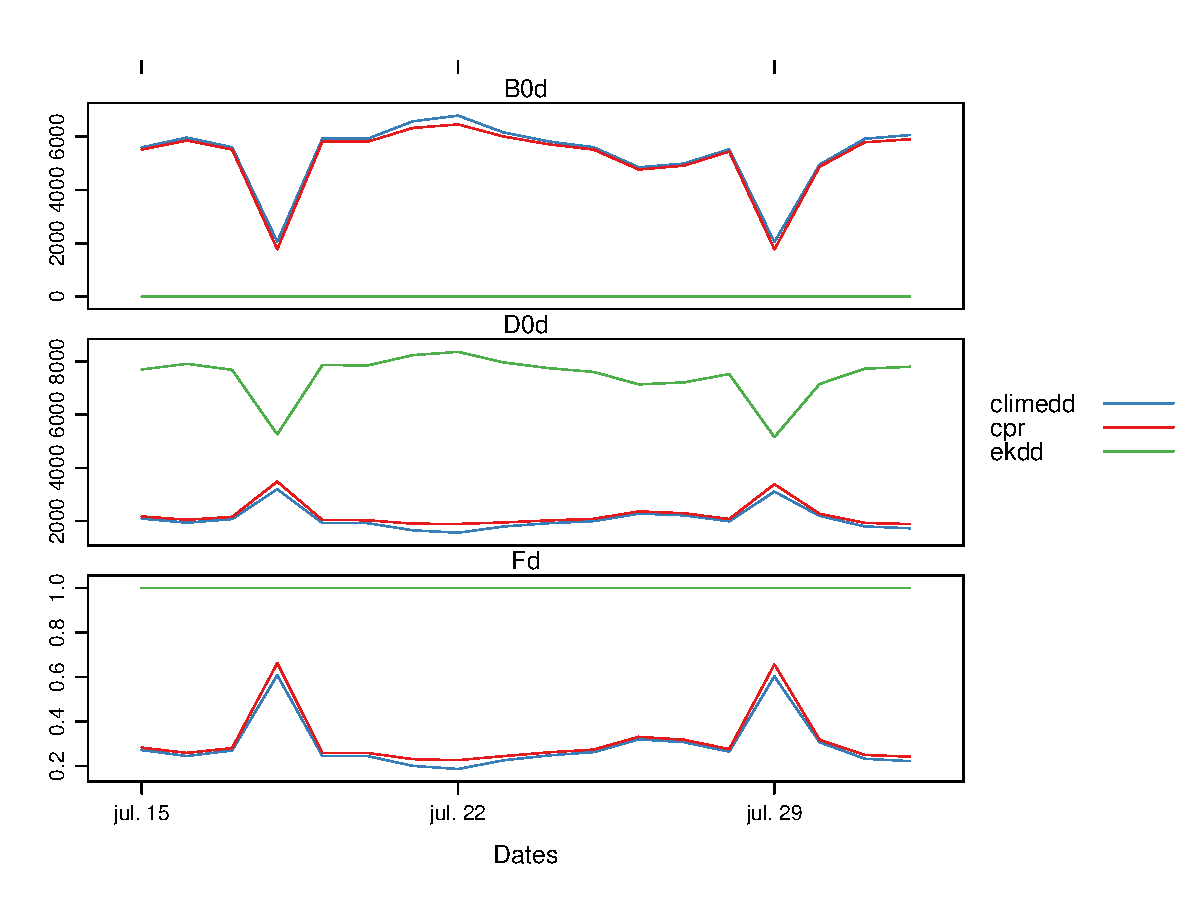
\includegraphics[width=0.8\textwidth]{figuras/codigo-fcompddia.pdf}
\end{center}
También, se puede aportar una función de correlación propia con el argumento \texttt{f}.
\begin{lstlisting}[numbers=left,language=r,label= ,caption= ,captionpos=b]
f_corrd <- function(sol, G0d){
  ## Función CLIMEDd
    Kt <- Ktd(sol, G0d)
    Fd=(Kt<=0.13)*(0.952)+
    (Kt>0.13 & Kt<=0.8)*(0.868+1.335*Kt-5.782*Kt^2+3.721*Kt^3)+
      (Kt>0.8)*0.141
  return(data.table(Fd, Kt))
}
compD_user <- fCompD(sol = sol, G0d = G0d, corr = 'user', f = f_corrd)
xyplot(compD_user)
\end{lstlisting}

\begin{center}
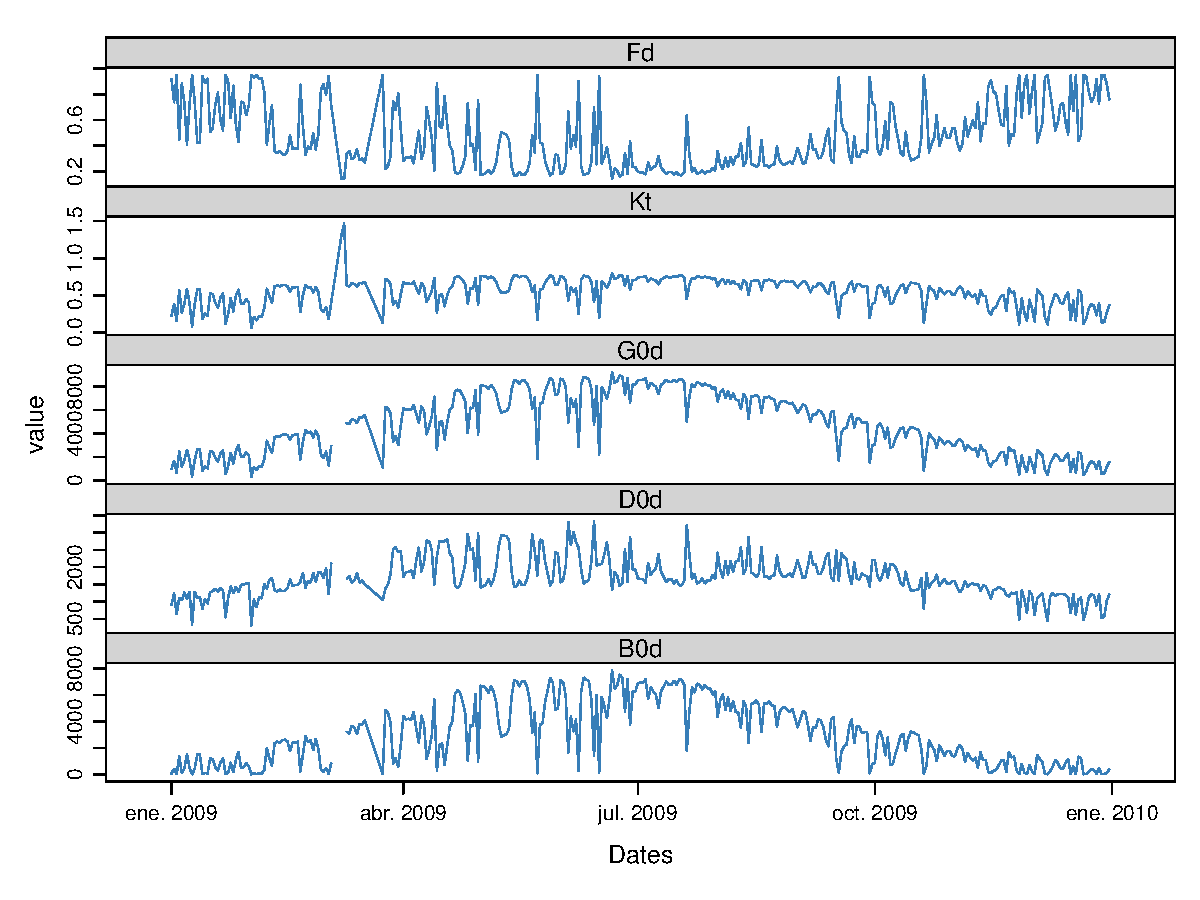
\includegraphics[width=0.8\textwidth]{figuras/codigo-fcompduser.pdf}
\end{center}
Por último, si \texttt{G0d} ya contiene todos los componentes, se puede especifica que no haga ninguna correlación.
\begin{lstlisting}[numbers=left,language=r,label= ,caption= ,captionpos=b]
compD_none <- fCompD(sol = sol, G0d = compD_user, corr = 'none')
compD_none
\end{lstlisting}

\begin{verbatim}
Key: <Dates>
	 Dates        Fd        Kt      G0d      D0d      B0d
	<POSc>     <num>     <num>    <num>    <num>    <num>
 1: 2024-07-15 0.2724591 0.6798139 7697.945 2097.375 5600.570
 2: 2024-07-16 0.2455880 0.7000272 7911.858 1943.057 5968.801
 3: 2024-07-17 0.2705287 0.6812283 7684.293 2078.822 5605.472
 4: 2024-07-18 0.6086148 0.4674993 5262.702 3202.958 2059.744
 5: 2024-07-19 0.2454217 0.7001561 7865.166 1930.282 5934.884
 6: 2024-07-20 0.2452020 0.7003266 7849.961 1924.826 5925.135
 7: 2024-07-21 0.2013208 0.7365959 8237.938 1658.468 6579.470
 8: 2024-07-22 0.1873678 0.7493438 8361.056 1566.592 6794.463
 9: 2024-07-23 0.2259736 0.7156288 7965.753 1800.050 6165.703
10: 2024-07-24 0.2483878 0.6978638 7748.845 1924.718 5824.126
11: 2024-07-25 0.2630540 0.6867564 7606.140 2000.826 5605.314
12: 2024-07-26 0.3202837 0.6462270 7138.548 2286.361 4852.187
13: 2024-07-27 0.3077503 0.6547900 7213.697 2220.018 4993.679
14: 2024-07-28 0.2653324 0.6850625 7526.355 1996.986 5529.369
15: 2024-07-29 0.6029930 0.4709412 5159.260 3110.998 2048.263
16: 2024-07-30 0.3076331 0.6548709 7153.359 2200.610 4952.749
17: 2024-07-31 0.2334298 0.7096003 7728.034 1803.954 5924.080
18: 2024-08-01 0.2224291 0.7185406 7801.435 1735.266 6066.168
\end{verbatim}
\end{itemize}

\item \texttt{fCompI}: calcula, en base a los valores de irradiación diaria, todas las componentes de irradiancia. Se vale de dos procedimientos en base al tipo de argumentos que toma:
\begin{itemize}
\item \texttt{compD}: Si recibe un \texttt{data.table} resultado de \texttt{fCompD}, calcula las relaciones entre las componentes de irradiancia e irradiación de las componentes de difusa y global, obteniendo con ellas un perfil de irradiancias [\ref{sec:radiacion-superficies-inclinadas}] (las irradiancias global y difusa salen de estas relaciones, mientras que la directa surge por diferencia entre las dos).
\end{itemize}
\begin{lstlisting}[numbers=left,language=r,label= ,caption= ,captionpos=b]
sol <- calcSol(lat = 37.2, BTd = fBTd(mode = 'prom'),
               sample = 'hour', keep.night = FALSE)
G0d <- c(2.766,3.491,4.494,5.912,6.989,7.742,7.919,
          7.027,5.369,3.562,2.814,2.179) * 1000
compD <- fCompD(sol = sol, G0d = G0d, corr = 'CPR')
compI <- fCompI(sol = sol, compD = compD)
xyplot(compI)
\end{lstlisting}

\begin{center}
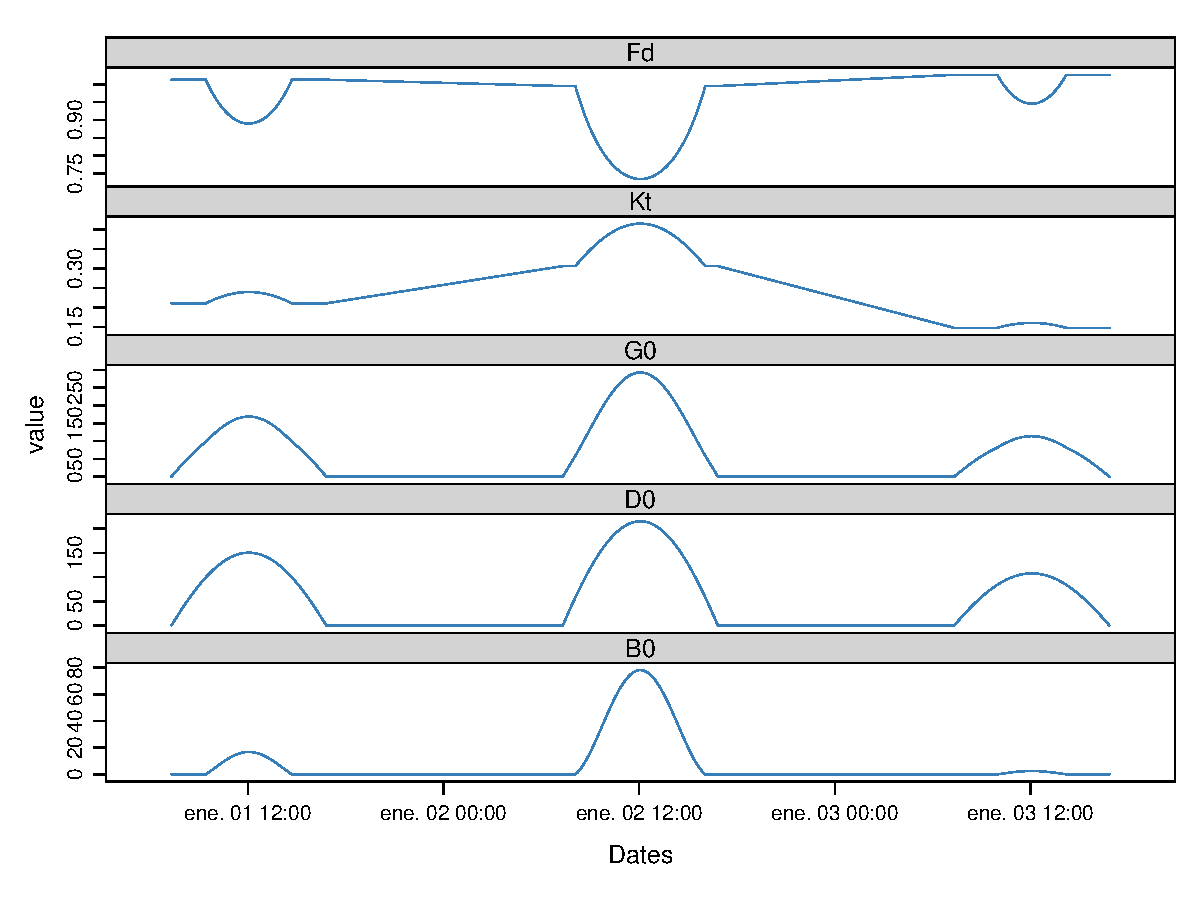
\includegraphics[width=0.8\textwidth]{figuras/codigo-fcompicompd.pdf}
\end{center}
\begin{itemize}
\item \texttt{G0I}: Este argumento recibe datos de irradiancia, para después, poder aplicar las correcciones indicadas en el argumento \texttt{corr}.
\end{itemize}
\begin{lstlisting}[numbers=left,language=r,label= ,caption= ,captionpos=b]
G0I <- compI$G0
compI_ekdh <- fCompI(sol = sol, G0I = G0I, corr = 'EKDh')
compI_ekdh[, group := 'ekdh']
compI_brl <- fCompI(sol = sol, G0I = G0I, corr = 'BRL')
compI_brl[, group := 'brl']
compI_climedh <- fCompI(sol = sol, G0I = G0I, corr = 'CLIMEDh')
compI_climedh[, group := 'climedh']
compI_all <- rbind(compI_ekdh, compI_ekdh, compI_climedh)
xyplot(Fd+ D0 +B0 ~ Dates, compI_all,
       groups= group, type = 'l',auto.key= TRUE,
       par.settings= solaR.theme,scales =list(y = 'free'),
       ylab = '', layout= c(1,3))
\end{lstlisting}

Como con \texttt{fCompD}, se puede añadir una función correctora propia.
\begin{lstlisting}[numbers=left,language=r,label= ,caption= ,captionpos=b]
f_corri <- function(sol, G0i){
  ## Función CLIMEDh
  Kt <- Kti(sol, G0i)
  Fd=(Kt<=0.21)*(0.995-0.081*Kt)+
    (Kt>0.21 & Kt<=0.76)*(0.724+2.738*Kt-8.32*Kt^2+4.967*Kt^3)+
    (Kt>0.76)*0.180
  return(data.table(Fd, Kt))
}
compI_user <- fCompI(sol = sol, G0I = G0I, corr = 'user', f = f_corri)
show(compI_user)
\end{lstlisting}

\begin{verbatim}
Key: <Dates>
		   Dates        Fd        Kt        G0        D0        B0
		  <POSc>     <num>     <num>     <num>     <num>     <num>
  1: 2024-01-17 08:00:00 0.7093252 0.4583592  84.06042  59.62617  24.43424
  2: 2024-01-17 09:00:00 0.5818534 0.5277148 215.49558 125.38683  90.10875
  3: 2024-01-17 10:00:00 0.4782729 0.5821268 340.45500 162.83039 177.62462
  4: 2024-01-17 11:00:00 0.4110389 0.6178887 433.04376 177.99784 255.04592
  5: 2024-01-17 12:00:00 0.3840268 0.6325646 473.44106 181.81406 291.62701
 ---                                                                      
141: 2024-12-13 12:00:00 0.5416063 0.5488870 382.71443 207.28055 175.43387
142: 2024-12-13 13:00:00 0.5639749 0.5371376 352.10710 198.57956 153.52754
143: 2024-12-13 14:00:00 0.6220088 0.5063725 276.60890 172.05317 104.55573
144: 2024-12-13 15:00:00 0.7087489 0.4586869 172.87432 122.52448  50.34984
145: 2024-12-13 16:00:00 0.8099691 0.3973283  63.15968  51.15739  12.00229
\end{verbatim}

Y además, se puede no añadir correlación.
\begin{lstlisting}[numbers=left,language=r,label= ,caption= ,captionpos=b]
G0I <- compI_user
compI_none <- fCompI(sol = sol, G0I = G0I, corr = 'none')
show(compI_none)
\end{lstlisting}

\begin{verbatim}
Key: <Dates>
		   Dates        Fd        Kt        G0        D0        B0
		  <POSc>     <num>     <num>     <num>     <num>     <num>
  1: 2024-01-17 08:00:00 0.7093252 0.4583592  84.06042  59.62617  24.43424
  2: 2024-01-17 09:00:00 0.5818534 0.5277148 215.49558 125.38683  90.10875
  3: 2024-01-17 10:00:00 0.4782729 0.5821268 340.45500 162.83039 177.62462
  4: 2024-01-17 11:00:00 0.4110389 0.6178887 433.04376 177.99784 255.04592
  5: 2024-01-17 12:00:00 0.3840268 0.6325646 473.44106 181.81406 291.62701
 ---                                                                      
141: 2024-12-13 12:00:00 0.5416063 0.5488870 382.71443 207.28055 175.43387
142: 2024-12-13 13:00:00 0.5639749 0.5371376 352.10710 198.57956 153.52754
143: 2024-12-13 14:00:00 0.6220088 0.5063725 276.60890 172.05317 104.55573
144: 2024-12-13 15:00:00 0.7087489 0.4586869 172.87432 122.52448  50.34984
145: 2024-12-13 16:00:00 0.8099691 0.3973283  63.15968  51.15739  12.00229
\end{verbatim}

Por útlimo, esta función incluye un argumento extra, \texttt{filterG0} que cuando su valor es \texttt{TRUE}, elimina todos aquellos valores de irradiancia que son mayores que la irradiancia extra-atmosfércia (ya que es incoherente que la irradiancia terrestre sea mayor que la extra-terrestre)
\end{itemize}

Estas dos funciones, como se muestra en la figura \ref{fig:calcg0}, convergen en la función constructora \texttt{calcG0}, dando como resultado un objeto de clase \texttt{G0}. Este objeto muestra la media mensual de la irradiación diaria y la irradiación anual. Aparte, incluye los resultados de \texttt{fCompD} y \texttt{fCompI} y los objetos \texttt{Sol} y \texttt{Meteo} de los que parte.

Como argumento más importante está \texttt{modeRad}, el cual selecciona el tipo de datos que introduce el usuario en el argumento \texttt{dataRad}. Estos son:
\begin{itemize}
\item Medias mensuales.
\begin{lstlisting}[numbers=left,language=r,label= ,caption= ,captionpos=b]
G0dm <- c(2.766, 3.491, 4.494, 5.912, 6.989, 7.742, 7.919,
          7.027, 5.369, 3.562, 2.814, 2.179) * 1000
Ta <- c(10, 14.1, 15.6, 17.2, 19.3, 21.2,
       28.4, 29.9, 24.3, 18.2, 17.2, 15.2)
prom <- data.table(G0dm, Ta) 
g0_prom <- calcG0(lat, modeRad = 'prom', dataRad = prom)
show(g0_prom)
\end{lstlisting}

\begin{verbatim}
Object of class  G0 

Source of meteorological information: prom- 

Latitude of source:  37.2 degrees
Latitude for calculations:  37.2 degrees

Monthly avarages:
	Dates   G0d      D0d      B0d
       <char> <num>    <num>    <num>
 1: Jan. 2024 2.766 0.941698 1.824302
 2: Feb. 2024 3.491 1.247146 2.243854
 3: Mar. 2024 4.494 1.671763 2.822237
 4: Apr. 2024 5.912 1.931146 3.980854
 5: May. 2024 6.989 2.023364 4.965636
 6: Jun. 2024 7.742 1.889994 5.852006
 7: Jul. 2024 7.919 1.624064 6.294936
 8: Aug. 2024 7.027 1.547591 5.479409
 9: Sep. 2024 5.369 1.540708 3.828292
10: Oct. 2024 3.562 1.374513 2.187487
11: Nov. 2024 2.814 1.006959 1.807041
12: Dec. 2024 2.179 0.926737 1.252263

Yearly values:
   Dates      G0d      D0d      B0d
   <int>    <num>    <num>    <num>
1:  2024 1839.365 540.6331 1298.732
\end{verbatim}

\item Generación de secuencias diarias mediante matrices de transición de Markov.
\begin{lstlisting}[numbers=left,language=r,label= ,caption= ,captionpos=b]
g0_aguiar <- calcG0(lat, modeRad = 'aguiar', dataRad = prom)
show(g0_aguiar)
\end{lstlisting}

\begin{verbatim}
Object of class  G0 

Source of meteorological information: bd-aguiar 

Latitude of source:  37.2 degrees
Latitude for calculations:  37.2 degrees

Monthly avarages:
	Dates   G0d      D0d       B0d
       <char> <num>    <num>     <num>
 1: Jan. 2024 2.766 1.087364 1.6786361
 2: Feb. 2024 3.491 1.494382 1.9966179
 3: Mar. 2024 4.494 2.073641 2.4203594
 4: Apr. 2024 5.912 2.373542 3.5384577
 5: May. 2024 6.989 2.431924 4.5570759
 6: Jun. 2024 7.742 2.429454 5.3125465
 7: Jul. 2024 7.919 2.311353 5.6076467
 8: Aug. 2024 7.027 2.175663 4.8513370
 9: Sep. 2024 5.369 1.880376 3.4886244
10: Oct. 2024 3.562 1.787310 1.7746900
11: Nov. 2024 2.814 1.315495 1.4985053
12: Dec. 2024 2.179 1.188310 0.9906898

Yearly values:
Key: <Dates>
   Dates      G0d      D0d      B0d
   <int>    <num>    <num>    <num>
1:  2024 1839.365 688.0256 1151.339
\end{verbatim}

\item Diarios.
\begin{lstlisting}[numbers=left,language=r,label= ,caption= ,captionpos=b]
bd <- as.data.tableD(g0_aguiar)
g0_bd <- calcG0(lat, modeRad = 'bd', dataRad = bd)
show(g0_bd)
\end{lstlisting}

\begin{verbatim}
Object of class  G0 

Source of meteorological information: bd-data.table 

Latitude of source:  37.2 degrees
Latitude for calculations:  37.2 degrees

Monthly avarages:
	Dates   G0d      D0d       B0d
       <char> <num>    <num>     <num>
 1: Jan. 2024 2.766 1.087364 1.6786361
 2: Feb. 2024 3.491 1.494382 1.9966179
 3: Mar. 2024 4.494 2.073641 2.4203594
 4: Apr. 2024 5.912 2.373542 3.5384577
 5: May. 2024 6.989 2.431924 4.5570759
 6: Jun. 2024 7.742 2.429454 5.3125465
 7: Jul. 2024 7.919 2.311353 5.6076467
 8: Aug. 2024 7.027 2.175663 4.8513370
 9: Sep. 2024 5.369 1.880376 3.4886244
10: Oct. 2024 3.562 1.787310 1.7746900
11: Nov. 2024 2.814 1.315495 1.4985053
12: Dec. 2024 2.179 1.188310 0.9906898

Yearly values:
Key: <Dates>
   Dates      G0d      D0d      B0d
   <int>    <num>    <num>    <num>
1:  2024 1839.365 688.0256 1151.339
\end{verbatim}

\item Intradiarios
\begin{lstlisting}[numbers=left,language=r,label= ,caption= ,captionpos=b]
bdI <- as.data.tableI(g0_aguiar)
g0_bdI <- calcG0(lat, modeRad = 'bdI', dataRad = bdI)
xyplot(g0_bdI)
\end{lstlisting}

\begin{center}
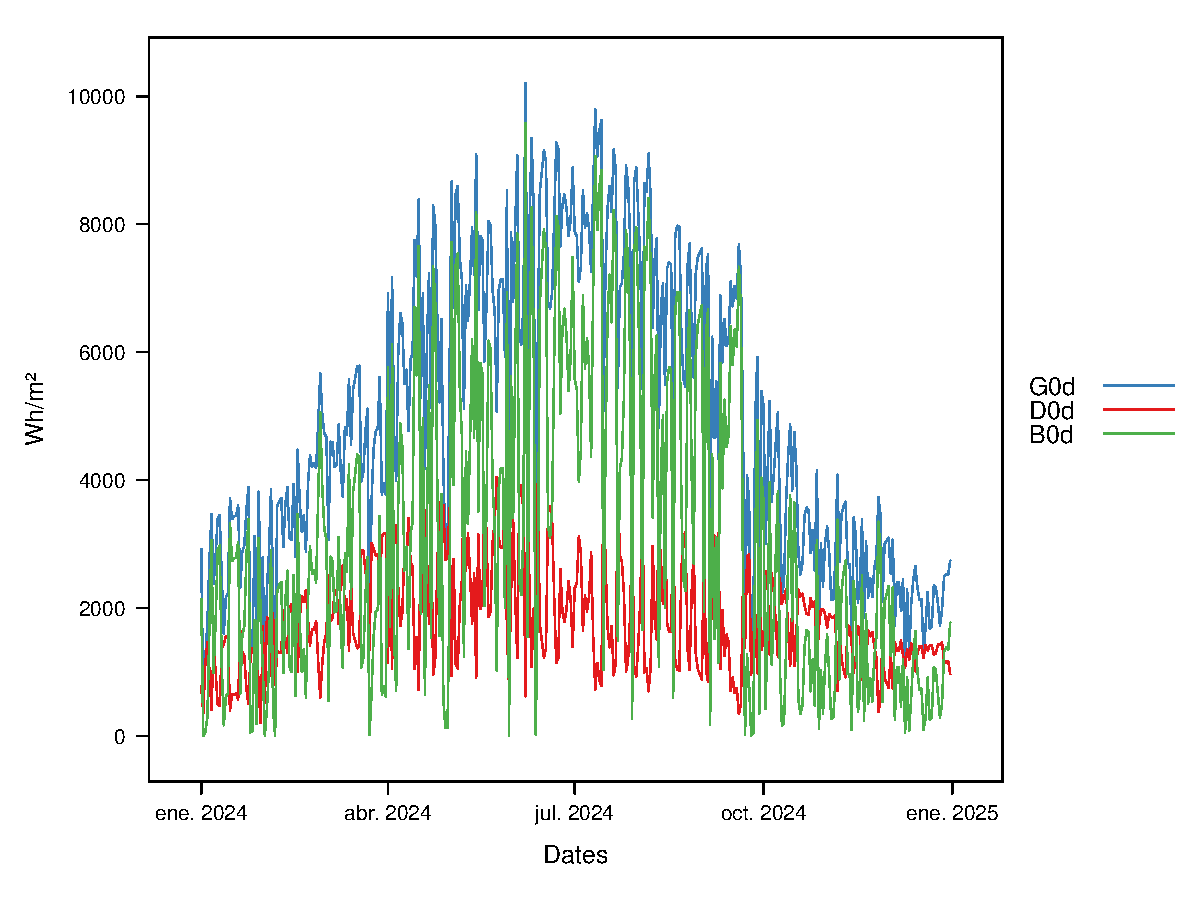
\includegraphics[width=0.8\textwidth]{figuras/codigo-calcg0.pdf}
\end{center}
\end{itemize}

\section{Radiación efectiva en el plano del generador}
\label{sec:org5fd0d3b}
\label{sec:radiacion-efectiva-plano-generador}
Teniendo la radiación incidente en plano horizontal (sección \ref{sec:radiacion-plano-horizontal}), se puede calcular la radiación efectiva incidente en el plano del generador. Para ello, \texttt{solaR2} cuenta con la función \texttt{calcGef} la cual mediante las funciones \texttt{fInclin} y \texttt{calcShd} procesa un objeto de clase \texttt{G0} para obtener un objeto \texttt{Gef}.

Como se puede ver en la figura \ref{fig:calcgef}, \texttt{calcGef} funciona gracias a las siguientes funciones:
\begin{figure}[htbp]
\centering
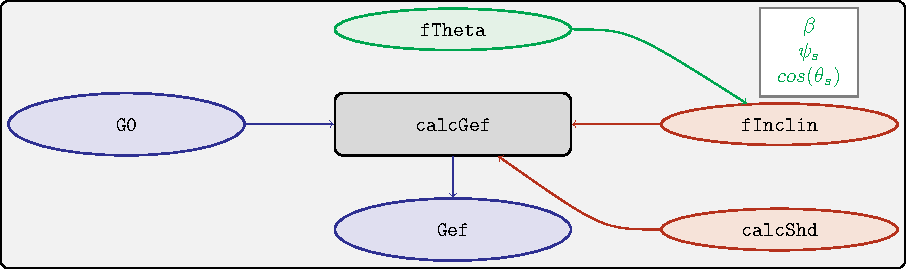
\includegraphics[keepaspectratio,width=\textwidth,height=0.5\textheight]{figuras/calcgef.pdf}
\caption{Cálculo de la radiación efectiva incidente en el plano del generador mediante la función \texttt{calcGef}, la cual emplea la función \texttt{fInclin} para el computo de las componentes efectivas, la función \texttt{fTheta} que provee a la función anterior los ángulos necesarios para su computo y la función \texttt{calcShd} que reprocesa el objeto de clase \texttt{Gef} resultante, añadiendole el efecto de las sombras producidas entres módulos. \label{fig:calcgef}}
\end{figure}
\begin{itemize}
\item \texttt{fTheta}: la cual, partiendo del ángulo de inclinación (\(\beta\)) y la orientación (\(\alpha\)), calcula el ángulo de inclinación en cada instante (\(\beta\)), el ángulo azimutal (\(\psi_s\)) y el coseno del ángulo de incidencia  de la radiación solar en la superficie (\(cos(\theta_s)\)).
Como principal argumento tiene \texttt{modeTrk}, el cual determina el sistema de seguimiento que tiene el sistema:
\begin{itemize}
\item \texttt{fixed}: para sistemas estáticos.
\end{itemize}
\begin{lstlisting}[numbers=left,language=r,label= ,caption= ,captionpos=b]
BTd <- fBTd(mode = 'serie')[1:10]
sol <- calcSol(lat, BTd = BTd, keep.night = FALSE)
beta <- lat - 10
alpha <- 0
angGen_fixed <- fTheta(sol = sol, beta = beta, alpha = alpha,
                       modeTrk = 'fixed')
xyplot(angGen_fixed)
\end{lstlisting}

\begin{center}
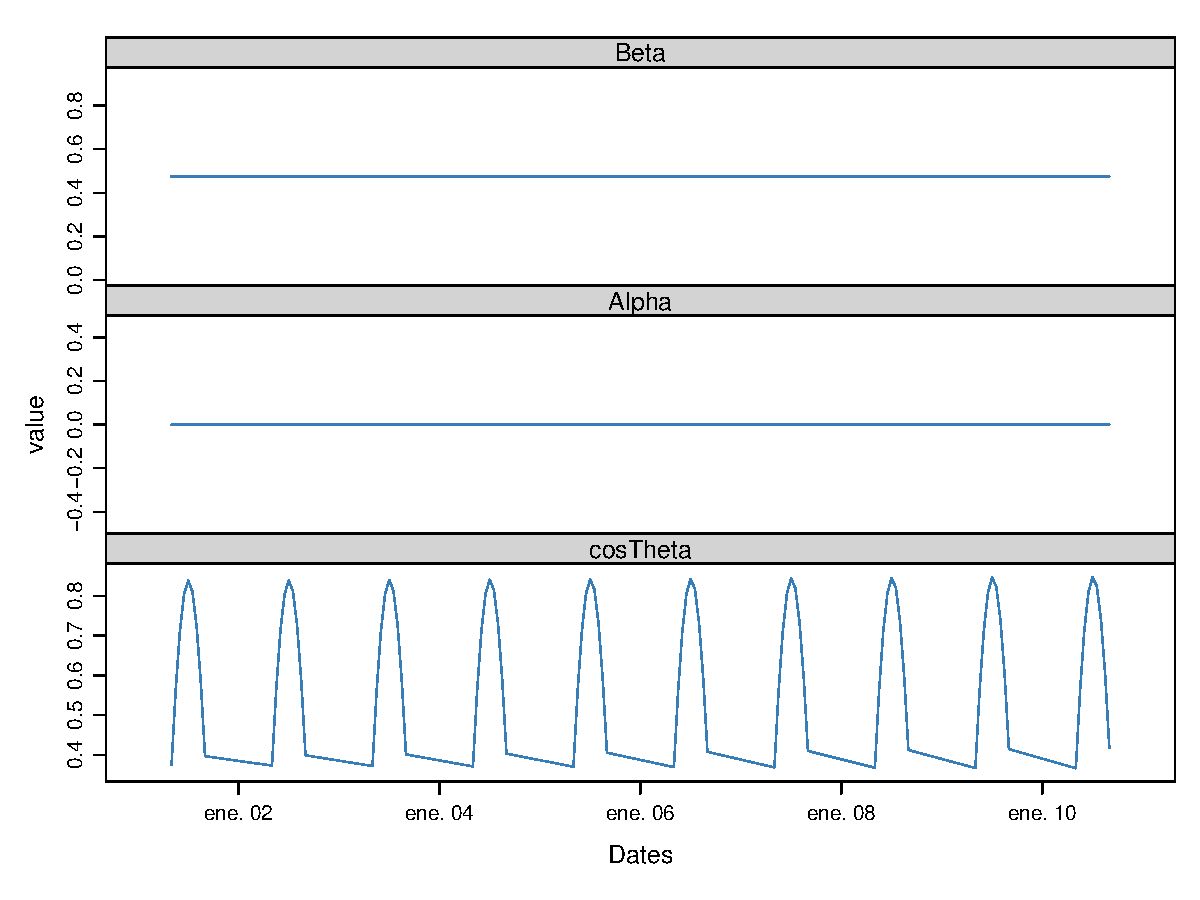
\includegraphics[width=0.8\textwidth]{figuras/codigo-fthetafixed.pdf}
\end{center}
\begin{itemize}
\item \texttt{two}: para sistemas de seguimiento de doble eje.
\end{itemize}
\begin{lstlisting}[numbers=left,language=r,label= ,caption= ,captionpos=b]
angGen_two <- fTheta(sol = sol, beta = beta, alpha = alpha,
                     modeTrk = 'two')
xyplot(angGen_two)
\end{lstlisting}

\begin{center}
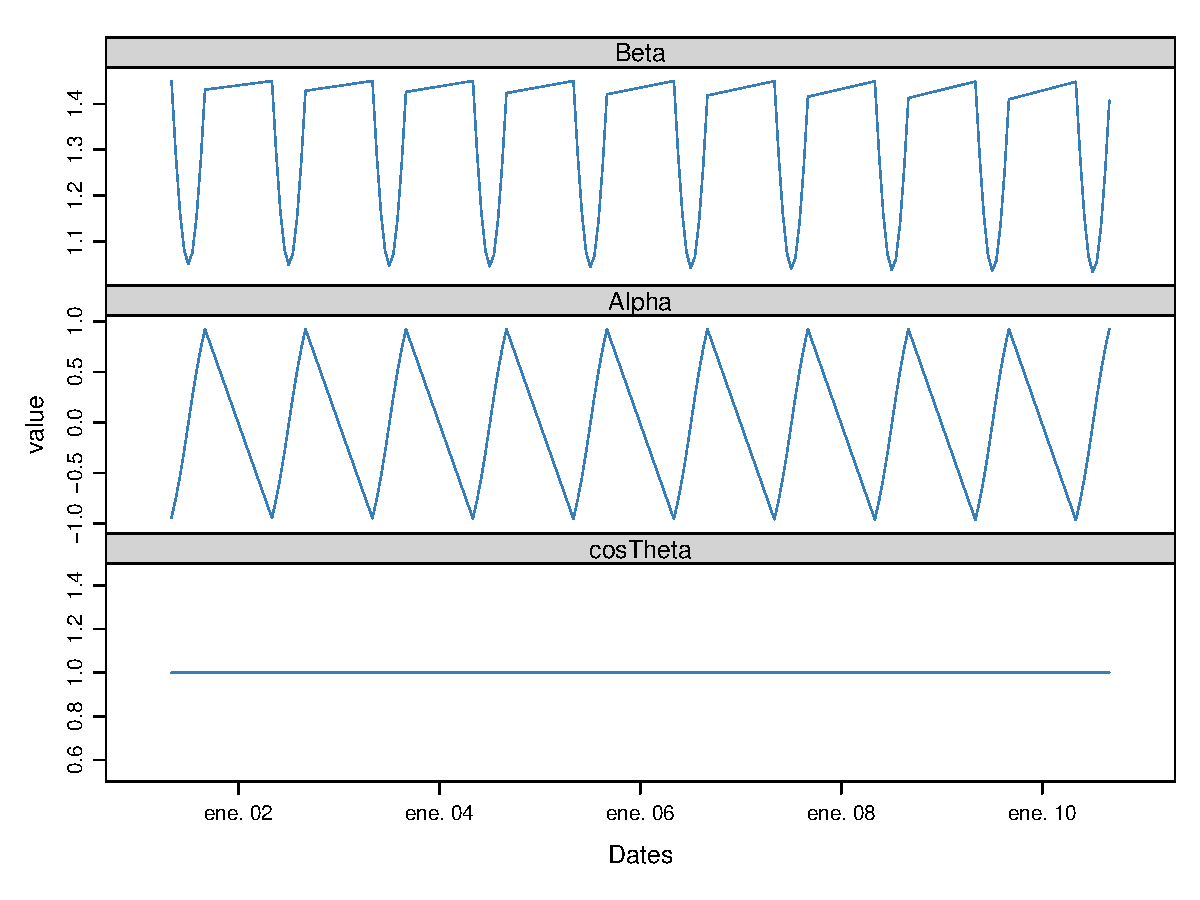
\includegraphics[width=0.8\textwidth]{figuras/codigo-fthetatwo.pdf}
\end{center}
\begin{itemize}
\item \texttt{horiz}: para sistemas de seguimiento horizontal Norte-Sur.
\end{itemize}
\begin{lstlisting}[numbers=left,language=r,label= ,caption= ,captionpos=b]
angGen_horiz <- fTheta(sol = sol, beta = beta, alpha = alpha,
                       modeTrk = 'horiz')
xyplot(angGen_horiz)
\end{lstlisting}

\begin{center}
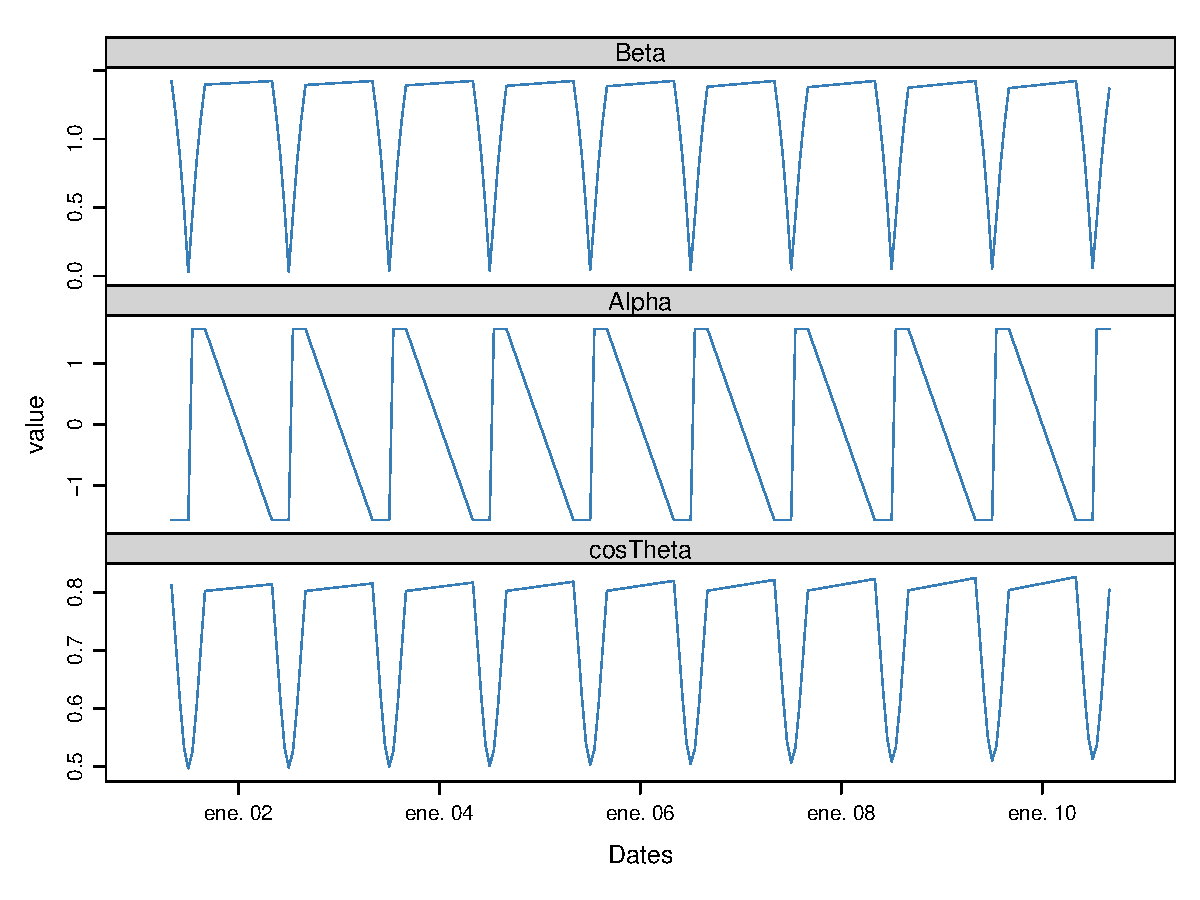
\includegraphics[width=0.8\textwidth]{figuras/codigo-fthetahoriz.pdf}
\end{center}
También, tiene un argumento \texttt{BT} que indica cuando se usa la técnica de backtracking para un sistema horizontal Norte-Sur. Para funcionar, necesita de los argumentos \texttt{struct}, el cual presenta una lista con la altura de los módulos, y \texttt{dist}, el cual presenta un \texttt{data.frame} (o \texttt{data.table}) con la distancia que separa los módulos en la dirección Este-Oeste.
\begin{lstlisting}[numbers=left,language=r,label= ,caption= ,captionpos=b]
struct <- list(L = 1)
distances <- data.table(Lew = 2)
angGen_BT <- fTheta(sol = sol, beta = beta, alpha = alpha,
                    modeTrk = 'horiz', BT = TRUE,
                    struct = struct, dist = distances)
xyplot(angGen_BT)
\end{lstlisting}

\begin{center}
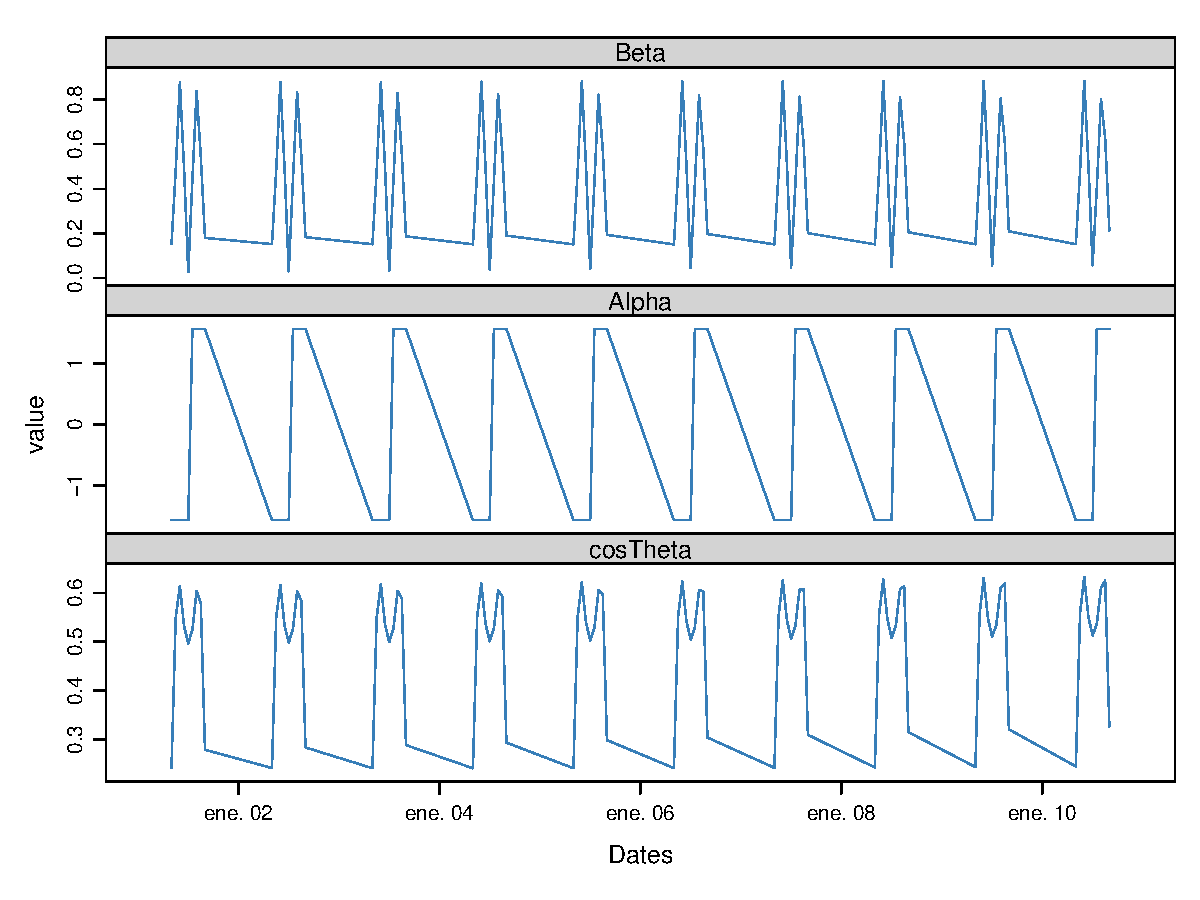
\includegraphics[width=0.8\textwidth]{figuras/codigo-fthetabt.pdf}
\end{center}
\item \texttt{fInclin}: la cual, partiendo del resultado de \texttt{fTheta} y de un objeto de clase \texttt{G0}, cálcula la irradiancia solar incidente en una superficie inclinada junto con los efectos del ángulo de incidencia y la suciedad para obtener la irradiancia efectiva.
Como argumentos principales están:
\begin{itemize}
\item \texttt{iS}: permite seleccionar entre 4 valores del 1 al 4 correspondientes al grado de suciedad del módulo. Siendo 1 limpio y 4 alto y basandose en los valores de la tabla \ref{tab:coef-perd} calcula la irradiancia efectiva. Por defecto tiene valor 2 (grado de suciedad bajo).
\end{itemize}
\begin{lstlisting}[numbers=left,language=r,label= ,caption= ,captionpos=b]
compI <- calcG0(lat, modeRad = 'bd', dataRad = bd[1:31], keep.night = FALSE)
sol <- calcSol(lat, BTi = indexI(compI))
angGen <- fTheta(sol = sol, beta = beta, alpha = alpha)
inclin_limpio <- fInclin(compI = compI, angGen = angGen, iS = 1)
inclin_limpio[, group := 'is = 1']
inclin_sucio <- fInclin(compI = compI, angGen = angGen, iS = 4)
inclin_sucio[, group := 'is = 4']
inclin_is <- rbind(inclin_limpio, inclin_sucio)
xyplot(Gef + Def + Bef + Ref ~ Dates, inclin_is,
       groups = group, type = 'l', auto.key = TRUE,
       par.settings = solaR.theme, scales = list(y = 'free'),
       ylab = '', layout = c(2, 2))
\end{lstlisting}

\begin{center}
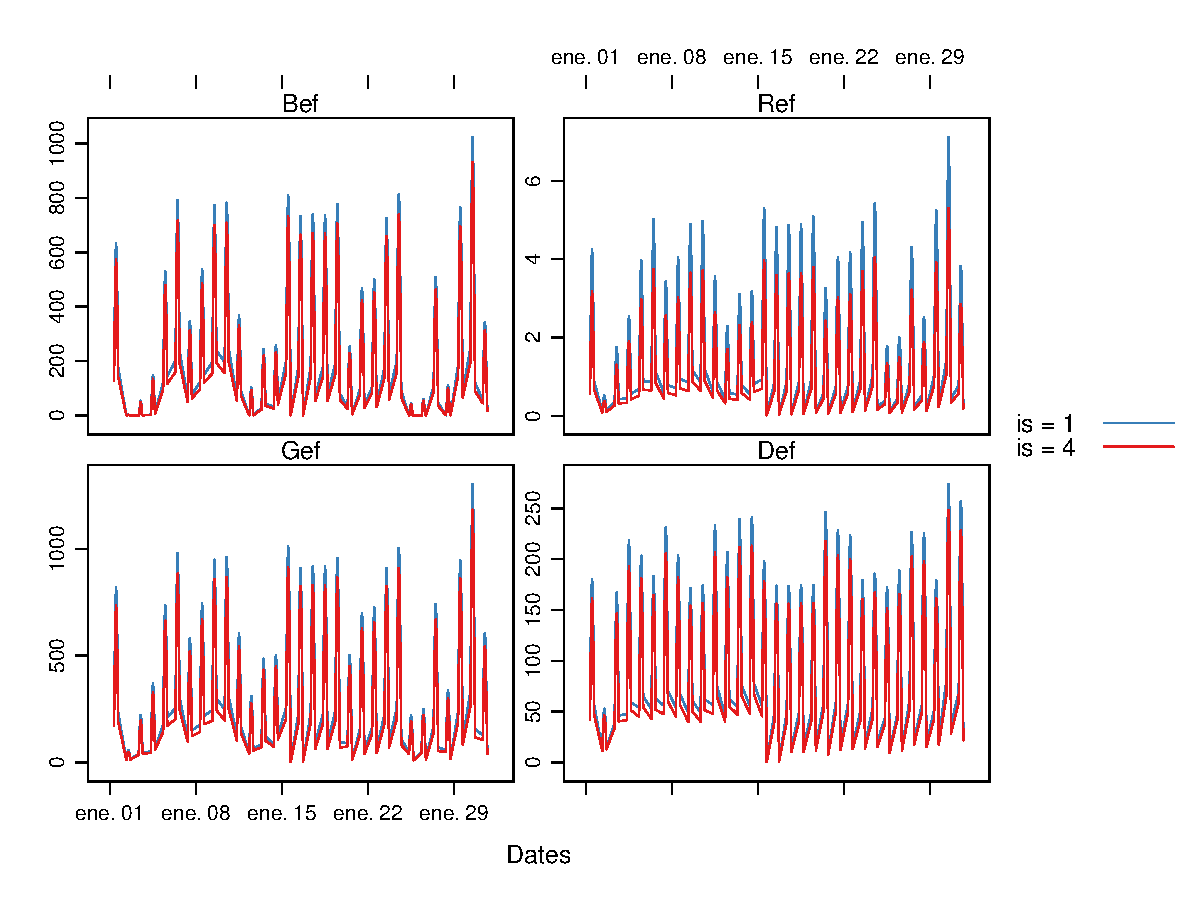
\includegraphics[width=0.8\textwidth]{figuras/codigo-finclinis.pdf}
\end{center}
\begin{itemize}
\item \texttt{alb} Correspondiente al coeficiente de reflexión del terreno para la irradiancia de albedo. Por defecto tiene un valor de 0,2 (valor aceptable para un terreno normal).
\end{itemize}
\begin{lstlisting}[numbers=left,language=r,label= ,caption= ,captionpos=b]
inclin_alb0 <- fInclin(compI = compI, angGen = angGen, alb = 0)
inclin_alb0[, group := 'alb = 0']
inclin_alb1 <- fInclin(compI = compI, angGen = angGen, alb = 1)
inclin_alb1[, group := 'alb = 1']
inclin_alb <- rbind(inclin_alb0, inclin_alb1)
xyplot(Gef + Def + Bef + Ref ~ Dates, inclin_alb,
       groups = group, type = 'l', auto.key = TRUE,
       par.settings = solaR.theme, scales = list(y = 'free'),
       ylab = '', layout = c(2, 2))
\end{lstlisting}

\begin{center}
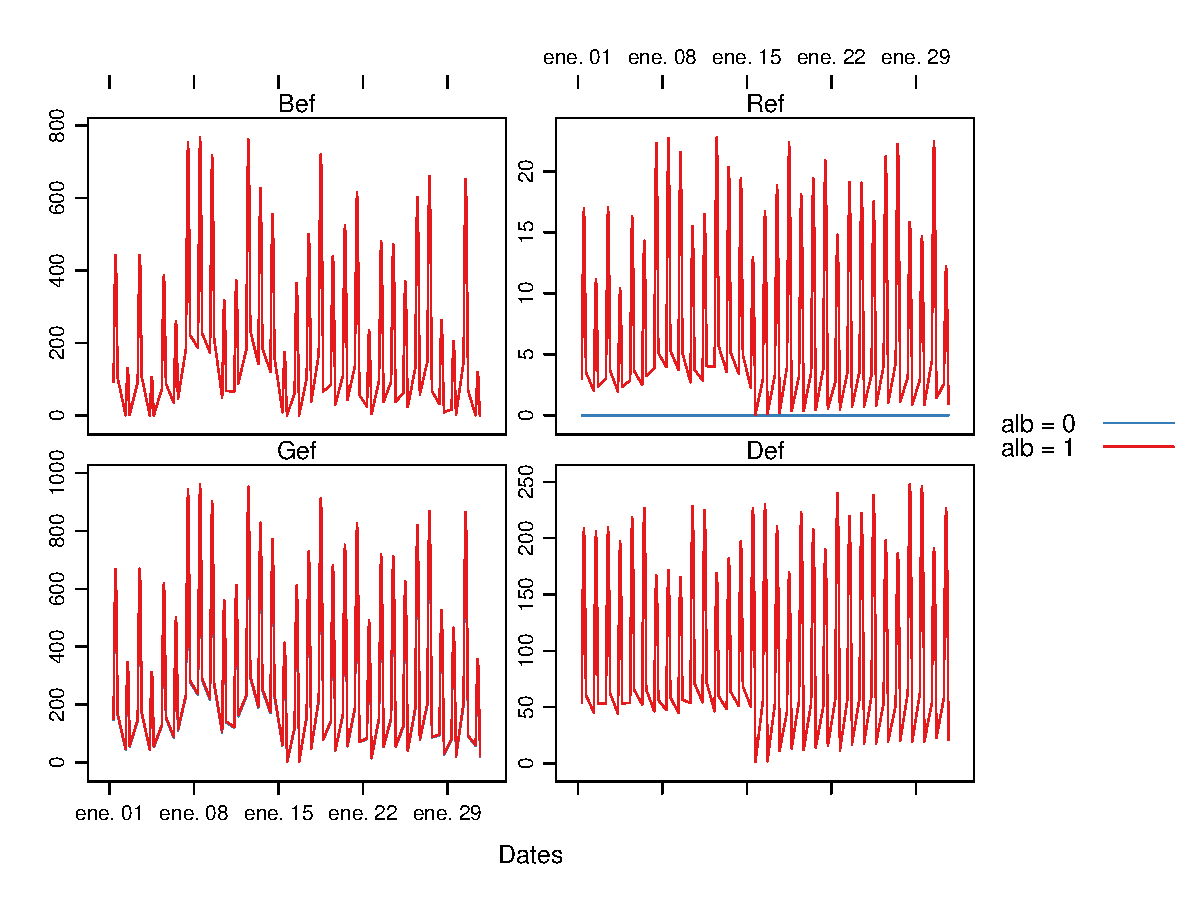
\includegraphics[width=0.8\textwidth]{figuras/codigo-finclinalb.pdf}
\end{center}
Además, cuenta con dos argumentos adicionales, \texttt{horizBright}, el cual, cuando su valor es \texttt{TRUE} (el que tiene por defecto), realiza una corrección de la radiación difusa \cite{REINDL19909}, y \texttt{HCPV}, es el acrónimo de \textbf{High Concentration PV system}\footnote{la tencología de concentración fotovoltaica funciona gracias a unos dispositivos ópticos que permiten concentrar la radiación solar sobre una célula fotovoltaica de tamaño reducido pero con una eficiencia muy superior alas células tradicionales. Con ello se consigue emplear menor cantidad de semiconductores reduciendo los costes.} (sistema fotovoltaico de alta concentración) que cuando su valor es \texttt{TRUE} (por defecto está puesto en \texttt{FALSE}), anula los valores de radiación difusa y de albedo.
\begin{lstlisting}[numbers=left,language=r,label= ,caption= ,captionpos=b]
inclin_horizBright <- fInclin(compI = compI, angGen = angGen,
                              horizBright = FALSE)
summary(inclin_horizBright)
\end{lstlisting}

\begin{verbatim}
    Dates                              Bo               Bn               G            
Min.   :2024-01-01 08:00:00.00   Min.   :   0.0   Min.   :   0.0   Min.   :   0.5136  
1st Qu.:2024-01-09 09:45:00.00   1st Qu.: 642.2   1st Qu.: 169.8   1st Qu.: 210.0040  
Median :2024-01-17 09:30:00.00   Median :1005.1   Median : 479.6   Median : 396.1338  
Mean   :2024-01-16 21:56:08.92   Mean   : 898.5   Mean   : 460.0   Mean   : 449.8593  
3rd Qu.:2024-01-24 13:15:00.00   3rd Qu.:1152.8   3rd Qu.: 740.8   3rd Qu.: 690.5324  
Max.   :2024-01-31 17:00:00.00   Max.   :1248.5   Max.   :1160.8   Max.   :1310.8339  
      D                 Di                Dc               B                 R         
Min.   :  0.488   Min.   :  0.488   Min.   :  0.00   Min.   :   0.00   Min.   :0.0256  
1st Qu.: 78.878   1st Qu.: 37.375   1st Qu.: 20.83   1st Qu.:  92.56   1st Qu.:1.3883  
Median :146.779   Median : 49.931   Median : 61.33   Median : 259.38   Median :3.0191  
Mean   :137.317   Mean   : 72.930   Mean   : 64.39   Mean   : 309.34   Mean   :3.2034  
3rd Qu.:182.864   3rd Qu.:107.437   3rd Qu.:101.46   3rd Qu.: 493.70   3rd Qu.:4.8652  
Max.   :275.542   Max.   :202.142   Max.   :243.53   Max.   :1025.81   Max.   :9.4826  
     FTb                FTd               FTr              Dief               Dcef       
Min.   :0.005218   Min.   :0.06474   Min.   :0.2995   Min.   :  0.4473   Min.   :  0.00  
1st Qu.:0.010325   1st Qu.:0.06474   1st Qu.:0.2995   1st Qu.: 34.2567   1st Qu.: 17.18  
Median :0.022076   Median :0.06474   Median :0.2995   Median : 45.7645   Median : 57.12  
Mean   :0.062300   Mean   :0.06474   Mean   :0.2995   Mean   : 66.8449   Mean   : 61.11  
3rd Qu.:0.096613   3rd Qu.:0.06474   3rd Qu.:0.2995   3rd Qu.: 98.4721   3rd Qu.: 98.16  
Max.   :0.344085   Max.   :0.06474   Max.   :0.2995   Max.   :185.2752   Max.   :237.38  
     Gef                 Def                Bef              Ref         
Min.   :   0.4648   Min.   :  0.4473   Min.   :  0.00   Min.   :0.01757  
1st Qu.: 194.5664   1st Qu.: 70.5638   1st Qu.: 72.15   1st Qu.:0.95309  
Median : 373.7350   Median :138.0750   Median :231.53   Median :2.07262  
Mean   : 423.5878   Mean   :127.9551   Mean   :293.43   Mean   :2.19917  
3rd Qu.: 661.6426   3rd Qu.:173.7286   3rd Qu.:477.84   3rd Qu.:3.33998  
Max.   :1273.1481   Max.   :266.7237   Max.   :999.91   Max.   :6.50988
\end{verbatim}

\begin{lstlisting}[numbers=left,language=r,label= ,caption= ,captionpos=b]
inclin_HCPV <- fInclin(compI = compI, angGen = angGen,
                       HCPV = TRUE)
summary(inclin_HCPV)
\end{lstlisting}

\begin{verbatim}
    Dates                              Bo               Bn               G            
Min.   :2024-01-01 08:00:00.00   Min.   :   0.0   Min.   :   0.0   Min.   :   0.5187  
1st Qu.:2024-01-09 09:45:00.00   1st Qu.: 642.2   1st Qu.: 169.8   1st Qu.: 210.6989  
Median :2024-01-17 09:30:00.00   Median :1005.1   Median : 479.6   Median : 397.2931  
Mean   :2024-01-16 21:56:08.92   Mean   : 898.5   Mean   : 460.0   Mean   : 450.4220  
3rd Qu.:2024-01-24 13:15:00.00   3rd Qu.:1152.8   3rd Qu.: 740.8   3rd Qu.: 691.1490  
Max.   :2024-01-31 17:00:00.00   Max.   :1248.5   Max.   :1160.8   Max.   :1311.2006  
      D                  Di                 Dc               B                 R         
Min.   :  0.4931   Min.   :  0.4931   Min.   :  0.00   Min.   :   0.00   Min.   :0.0256  
1st Qu.: 79.1629   1st Qu.: 37.7934   1st Qu.: 20.83   1st Qu.:  92.56   1st Qu.:1.3883  
Median :147.4695   Median : 50.2948   Median : 61.33   Median : 259.38   Median :3.0191  
Mean   :137.8795   Mean   : 73.4931   Mean   : 64.39   Mean   : 309.34   Mean   :3.2034  
3rd Qu.:183.4776   3rd Qu.:108.2063   3rd Qu.:101.46   3rd Qu.: 493.70   3rd Qu.:4.8652  
Max.   :275.9089   Max.   :203.4060   Max.   :243.53   Max.   :1025.81   Max.   :9.4826  
     FTb                FTd               FTr              Dief        Dcef        Gef        
Min.   :0.005218   Min.   :0.06474   Min.   :0.2995   Min.   :0   Min.   :0   Min.   :  0.00  
1st Qu.:0.010325   1st Qu.:0.06474   1st Qu.:0.2995   1st Qu.:0   1st Qu.:0   1st Qu.: 72.15  
Median :0.022076   Median :0.06474   Median :0.2995   Median :0   Median :0   Median :231.53  
Mean   :0.062300   Mean   :0.06474   Mean   :0.2995   Mean   :0   Mean   :0   Mean   :293.43  
3rd Qu.:0.096613   3rd Qu.:0.06474   3rd Qu.:0.2995   3rd Qu.:0   3rd Qu.:0   3rd Qu.:477.84  
Max.   :0.344085   Max.   :0.06474   Max.   :0.2995   Max.   :0   Max.   :0   Max.   :999.91  
     Def         Bef              Ref   
Min.   :0   Min.   :  0.00   Min.   :0  
1st Qu.:0   1st Qu.: 72.15   1st Qu.:0  
Median :0   Median :231.53   Median :0  
Mean   :0   Mean   :293.43   Mean   :0  
3rd Qu.:0   3rd Qu.:477.84   3rd Qu.:0  
Max.   :0   Max.   :999.91   Max.   :0
\end{verbatim}
\end{itemize}

Finalmente, esta función le otorga estos datos a la función \texttt{calcGef} para que produzca un objeto de clase \texttt{Gef} como resultado. Esta función tiene como argumentos principales los mismos que los que tiene \texttt{calcG0} \ref{sec:radiacion-plano-horizontal}, es decir, \texttt{modeRad} y \texttt{dataRad}. Y además, como es lógico, con todos los argumentos mencionados con anterioridad en \texttt{fTheta} y \texttt{fInclin}.
\begin{lstlisting}[numbers=left,language=r,label= ,caption= ,captionpos=b]
gef_prom <- calcGef(lat = lat, modeTrk = 'two', modeRad = 'prom',
                    dataRad = prom,
                    beta = lat-10, alpha = 0,
                    iS = 2, alb = 0.2,
                    horizBright = TRUE, HCPV = FALSE)
show(gef_prom)
\end{lstlisting}

\begin{verbatim}
Object of class  Gef 

Source of meteorological information: prom- 

Latitude of source:  37.2 degrees
Latitude for calculations:  37.2 degrees

Monthly avarages:
        Dates      Bod       Bnd        Gd       Dd       Bd      Gefd     Defd     Befd
       <char>    <num>     <num>     <num>    <num>    <num>     <num>    <num>    <num>
 1: Jan. 2024 14.13536  4.924221  6.522313 1.440413 4.924221  6.348801 1.384087 4.825736
 2: Feb. 2024 15.42754  5.034287  6.875052 1.672079 5.034287  6.680139 1.599929 4.933601
 3: Mar. 2024 16.58107  5.163713  7.329138 1.998110 5.163713  7.104641 1.902356 5.060439
 4: Apr. 2024 17.64047  6.408617  8.843422 2.265896 6.408617  8.578222 2.158071 6.280444
 5: May. 2024 18.70771  7.617499 10.178196 2.394606 7.617499  9.885240 2.284334 7.465149
 6: Jun. 2024 19.87238  9.102430 11.606533 2.329653 9.102430 11.293417 2.230338 8.920381
 7: Jul. 2024 18.51695 10.037233 11.801533 2.029150 9.589205 11.495648 1.948530 9.397421
 8: Aug. 2024 17.34098  8.640959 10.777404 1.947410 8.640959 10.493150 1.869393 8.468140
 9: Sep. 2024 16.25295  6.698488  8.831006 1.948075 6.698488  8.584604 1.864962 6.564518
10: Oct. 2024 15.16994  4.546024  6.418653 1.711039 4.546024  6.226290 1.631551 4.455104
11: Nov. 2024 14.00493  4.638289  6.247341 1.452953 4.638289  6.076159 1.393353 4.545523
12: Dec. 2024 12.70717  3.439788  4.825181 1.254616 3.439788  4.685547 1.198824 3.370992

Yearly values:
   Dates      Bod      Bnd       Gd       Dd       Bd     Gefd    Defd     Befd
   <int>    <num>    <num>    <num>    <num>    <num>    <num>   <num>    <num>
1:  2024 5988.455 2326.882 3058.651 684.4232 2312.993 2973.115 654.591 2266.733
-----------------
Mode of tracking:  two 
    Inclination limit: 90
\end{verbatim}

Sin embargo, como argumento importante está \texttt{modeShd}, el cual permite incluir el efecto de las sombras entre módulos al objeto \texttt{Gef} mediante el uso de la función \texttt{calcShd}. Esta opción añade las variables \texttt{Gef0}, \texttt{Def0} y \texttt{Bef0} las cuales son las componentes de radiación efectiva previas a aplicar el efecto de las sombras con el fin de poder comparar.
\begin{lstlisting}[numbers=left,language=r,label= ,caption= ,captionpos=b]
struct <- list(W=23.11, L=9.8, Nrow=2, Ncol=8)
distances <- data.table(Lew=40, Lns=30, H=0)
gef_shd <- calcShd(radEf = gef_prom, modeShd = 'prom',
                   struct = struct, distances = distances)
show(gef_shd)
\end{lstlisting}

\begin{verbatim}
Object of class  Gef 

Source of meteorological information: prom- 

Latitude of source:  37.2 degrees
Latitude for calculations:  37.2 degrees

Monthly avarages:
        Dates     Gef0d    Def0d    Bef0d        Gd       Dd       Bd      Gefd     Defd     Befd
       <char>     <num>    <num>    <num>     <num>    <num>    <num>     <num>    <num>    <num>
 1: Jan. 2024  6.348801 1.384087 4.825736  6.522313 1.440413 4.924221  6.104126 1.343455 4.621693
 2: Feb. 2024  6.680139 1.599929 4.933601  6.875052 1.672079 5.034287  6.406274 1.553670 4.705996
 3: Mar. 2024  7.104641 1.902356 5.060439  7.329138 1.998110 5.163713  6.788630 1.848127 4.798657
 4: Apr. 2024  8.578222 2.158071 6.280444  8.843422 2.265896 6.408617  8.295340 2.112064 6.043569
 5: May. 2024  9.885240 2.284334 7.465149 10.178196 2.394606 7.617499  9.688308 2.253942 7.298609
 6: Jun. 2024 11.293417 2.230338 8.920381 11.606533 2.329653 9.102430 11.115054 2.205314 8.767042
 7: Jul. 2024 11.495648 1.948530 9.397421 11.801533 2.029150 9.589205 11.308971 1.924962 9.234312
 8: Aug. 2024 10.493150 1.869393 8.468140 10.777404 1.947410 8.640959 10.196758 1.830334 8.210807
 9: Sep. 2024  8.584604 1.864962 6.564518  8.831006 1.948075 6.698488  8.228309 1.810198 6.262986
10: Oct. 2024  6.226290 1.631551 4.455104  6.418653 1.711039 4.546024  6.018374 1.595528 4.283212
11: Nov. 2024  6.076159 1.393353 4.545523  6.247341 1.452953 4.638289  5.875732 1.359514 4.378935
12: Dec. 2024  4.685547 1.198824 3.370992  4.825181 1.254616 3.439788  4.575893 1.179346 3.280817

Yearly values:
   Dates    Gef0d   Def0d    Bef0d       Gd       Dd       Bd     Gefd     Defd     Befd
   <int>    <num>   <num>    <num>    <num>    <num>    <num>    <num>    <num>    <num>
1:  2024 2973.115 654.591 2266.733 3058.651 684.4232 2312.993 2886.328 640.9157 2193.621
-----------------
Mode of tracking:  two 
    Inclination limit: 90
\end{verbatim}

\begin{lstlisting}[numbers=left,language=r,label= ,caption= ,captionpos=b]
gef_shd2 <- calcGef(lat = lat, modeTrk = 'two', dataRad = prom,
                    modeShd = 'prom', struct = struct, distances = distances)
show(gef_shd2)
\end{lstlisting}

\begin{verbatim}
Object of class  Gef 

Source of meteorological information: prom- 

Latitude of source:  37.2 degrees
Latitude for calculations:  37.2 degrees

Monthly avarages:
        Dates     Gef0d    Def0d    Bef0d        Gd       Dd       Bd      Gefd     Defd     Befd
       <char>     <num>    <num>    <num>     <num>    <num>    <num>     <num>    <num>    <num>
 1: Jan. 2024  6.348801 1.384087 4.825736  6.522313 1.440413 4.924221  6.104126 1.343455 4.621693
 2: Feb. 2024  6.680139 1.599929 4.933601  6.875052 1.672079 5.034287  6.406274 1.553670 4.705996
 3: Mar. 2024  7.104641 1.902356 5.060439  7.329138 1.998110 5.163713  6.788630 1.848127 4.798657
 4: Apr. 2024  8.578222 2.158071 6.280444  8.843422 2.265896 6.408617  8.295340 2.112064 6.043569
 5: May. 2024  9.885240 2.284334 7.465149 10.178196 2.394606 7.617499  9.688308 2.253942 7.298609
 6: Jun. 2024 11.293417 2.230338 8.920381 11.606533 2.329653 9.102430 11.115054 2.205314 8.767042
 7: Jul. 2024 11.495648 1.948530 9.397421 11.801533 2.029150 9.589205 11.308971 1.924962 9.234312
 8: Aug. 2024 10.493150 1.869393 8.468140 10.777404 1.947410 8.640959 10.196758 1.830334 8.210807
 9: Sep. 2024  8.584604 1.864962 6.564518  8.831006 1.948075 6.698488  8.228309 1.810198 6.262986
10: Oct. 2024  6.226290 1.631551 4.455104  6.418653 1.711039 4.546024  6.018374 1.595528 4.283212
11: Nov. 2024  6.076159 1.393353 4.545523  6.247341 1.452953 4.638289  5.875732 1.359514 4.378935
12: Dec. 2024  4.685547 1.198824 3.370992  4.825181 1.254616 3.439788  4.575893 1.179346 3.280817

Yearly values:
   Dates    Gef0d   Def0d    Bef0d       Gd       Dd       Bd     Gefd     Defd     Befd
   <int>    <num>   <num>    <num>    <num>    <num>    <num>    <num>    <num>    <num>
1:  2024 2973.115 654.591 2266.733 3058.651 684.4232 2312.993 2886.328 640.9157 2193.621
-----------------
Mode of tracking:  two 
    Inclination limit: 90
\end{verbatim}

El argumento \texttt{modeShd} puede ser de distintas maneras:
\begin{itemize}
\item \texttt{area}: el efecto de las sombras se calcula como una reducción proporcional de las irradiancias difusa circunsolar y directa.
\end{itemize}
\begin{lstlisting}[numbers=left,language=r,label= ,caption= ,captionpos=b]
gef_shdarea <- calcGef(lat, modeTrk = 'two', dataRad = prom,
                       modeShd = 'area',
                       struct = struct, distances = distances)
show(gef_shdarea)
\end{lstlisting}

\begin{verbatim}
Object of class  Gef 

Source of meteorological information: prom- 

Latitude of source:  37.2 degrees
Latitude for calculations:  37.2 degrees

Monthly avarages:
        Dates     Gef0d    Def0d    Bef0d        Gd       Dd       Bd      Gefd     Defd     Befd
       <char>     <num>    <num>    <num>     <num>    <num>    <num>     <num>    <num>    <num>
 1: Jan. 2024  6.348801 1.384087 4.825736  6.522313 1.440413 4.924221  5.877879 1.305883 4.433019
 2: Feb. 2024  6.680139 1.599929 4.933601  6.875052 1.672079 5.034287  6.291348 1.534257 4.610483
 3: Mar. 2024  7.104641 1.902356 5.060439  7.329138 1.998110 5.163713  6.743478 1.840379 4.761253
 4: Apr. 2024  8.578222 2.158071 6.280444  8.843422 2.265896 6.408617  8.254928 2.105491 6.009730
 5: May. 2024  9.885240 2.284334 7.465149 10.178196 2.394606 7.617499  9.660175 2.249601 7.274817
 6: Jun. 2024 11.293417 2.230338 8.920381 11.606533 2.329653 9.102430 11.089573 2.201739 8.745137
 7: Jul. 2024 11.495648 1.948530 9.397421 11.801533 2.029150 9.589205 11.282303 1.921596 9.211011
 8: Aug. 2024 10.493150 1.869393 8.468140 10.777404 1.947410 8.640959 10.154416 1.824754 8.174045
 9: Sep. 2024  8.584604 1.864962 6.564518  8.831006 1.948075 6.698488  8.177410 1.802375 6.219910
10: Oct. 2024  6.226290 1.631551 4.455104  6.418653 1.711039 4.546024  5.950189 1.583714 4.226840
11: Nov. 2024  6.076159 1.393353 4.545523  6.247341 1.452953 4.638289  5.705306 1.330740 4.237284
12: Dec. 2024  4.685547 1.198824 3.370992  4.825181 1.254616 3.439788  4.440179 1.155239 3.169210

Yearly values:
   Dates    Gef0d   Def0d    Bef0d       Gd       Dd       Bd     Gefd     Defd     Befd
   <int>    <num>   <num>    <num>    <num>    <num>    <num>    <num>    <num>    <num>
1:  2024 2973.115 654.591 2266.733 3058.651 684.4232 2312.993 2856.633 636.0199 2168.822
-----------------
Mode of tracking:  two 
    Inclination limit: 90
\end{verbatim}

\begin{itemize}
\item \texttt{prom}: cuando \texttt{modeTrk} es \texttt{two}, se puede calcular el efecto de las sombras de un seguidor promedio.
\end{itemize}
\begin{lstlisting}[numbers=left,language=r,label= ,caption= ,captionpos=b]
gef_shdprom <- calcGef(lat, modeTrk = 'two', dataRad = prom,
                       modeShd = c('area', 'prom'),
                       struct = struct, distances = distances)
show(gef_shdprom)
\end{lstlisting}

\begin{verbatim}
Object of class  Gef 

Source of meteorological information: prom- 

Latitude of source:  37.2 degrees
Latitude for calculations:  37.2 degrees

Monthly avarages:
        Dates     Gef0d    Def0d    Bef0d        Gd       Dd       Bd      Gefd     Defd     Befd
       <char>     <num>    <num>    <num>     <num>    <num>    <num>     <num>    <num>    <num>
 1: Jan. 2024  6.348801 1.384087 4.825736  6.522313 1.440413 4.924221  6.104126 1.343455 4.621693
 2: Feb. 2024  6.680139 1.599929 4.933601  6.875052 1.672079 5.034287  6.406274 1.553670 4.705996
 3: Mar. 2024  7.104641 1.902356 5.060439  7.329138 1.998110 5.163713  6.788630 1.848127 4.798657
 4: Apr. 2024  8.578222 2.158071 6.280444  8.843422 2.265896 6.408617  8.295340 2.112064 6.043569
 5: May. 2024  9.885240 2.284334 7.465149 10.178196 2.394606 7.617499  9.688308 2.253942 7.298609
 6: Jun. 2024 11.293417 2.230338 8.920381 11.606533 2.329653 9.102430 11.115054 2.205314 8.767042
 7: Jul. 2024 11.495648 1.948530 9.397421 11.801533 2.029150 9.589205 11.308971 1.924962 9.234312
 8: Aug. 2024 10.493150 1.869393 8.468140 10.777404 1.947410 8.640959 10.196758 1.830334 8.210807
 9: Sep. 2024  8.584604 1.864962 6.564518  8.831006 1.948075 6.698488  8.228309 1.810198 6.262986
10: Oct. 2024  6.226290 1.631551 4.455104  6.418653 1.711039 4.546024  6.018374 1.595528 4.283212
11: Nov. 2024  6.076159 1.393353 4.545523  6.247341 1.452953 4.638289  5.875732 1.359514 4.378935
12: Dec. 2024  4.685547 1.198824 3.370992  4.825181 1.254616 3.439788  4.575893 1.179346 3.280817

Yearly values:
   Dates    Gef0d   Def0d    Bef0d       Gd       Dd       Bd     Gefd     Defd     Befd
   <int>    <num>   <num>    <num>    <num>    <num>    <num>    <num>    <num>    <num>
1:  2024 2973.115 654.591 2266.733 3058.651 684.4232 2312.993 2886.328 640.9157 2193.621
-----------------
Mode of tracking:  two 
    Inclination limit: 90
\end{verbatim}

\begin{itemize}
\item \texttt{bt}: cuando \texttt{modeTrk} es \texttt{horiz}, se puede calcular el efecto del \emph{backtracking} en las sombras.
\end{itemize}
\begin{lstlisting}[numbers=left,language=r,label= ,caption= ,captionpos=b]
gef_shdhoriz <- calcGef(lat, modeTrk = 'horiz', dataRad = prom,
                        modeShd = 'area',
                        struct = struct, distances = distances)
show(gef_shdhoriz)
\end{lstlisting}

\begin{verbatim}
Object of class  Gef 

Source of meteorological information: prom- 

Latitude of source:  37.2 degrees
Latitude for calculations:  37.2 degrees

Monthly avarages:
        Dates     Gef0d     Def0d    Bef0d        Gd       Dd       Bd      Gefd      Defd     Befd
       <char>     <num>     <num>    <num>     <num>    <num>    <num>     <num>     <num>    <num>
 1: Jan. 2024  4.274445 1.0909303 3.118987  4.528022 1.166334 3.285391  3.826940 1.0166151 2.745797
 2: Feb. 2024  5.173537 1.3974587 3.699745  5.414413 1.484046 3.839622  4.709780 1.3191237 3.314324
 3: Mar. 2024  6.270377 1.8008592 4.379272  6.512568 1.906181 4.498391  5.856407 1.7298195 4.036342
 4: Apr. 2024  8.160354 2.1103041 5.938446  8.429640 2.222836 6.072611  7.744288 2.0426359 5.590049
 5: May. 2024  9.639011 2.2544315 7.260788  9.932830 2.366831 7.416258  9.158384 2.1802588 6.854334
 6: Jun. 2024 11.005388 2.1942042 8.675874 11.320680 2.294944 8.861907 10.355140 2.1029750 8.116855
 7: Jul. 2024 11.220872 1.9183453 9.163290 11.527430 2.000253 9.358648 10.747413 1.8585724 8.749603
 8: Aug. 2024 10.066277 1.8239013 8.112148 10.352216 1.904515 8.290847  9.601132 1.7626031 7.708301
 9: Sep. 2024  7.732062 1.7621525 5.864625  7.991813 1.852070 6.013507  7.317424 1.6984219 5.513717
10: Oct. 2024  5.023316 1.4757157 3.471271  5.250215 1.568278 3.591050  4.691499 1.4182254 3.196944
11: Nov. 2024  4.211801 1.1318865 3.014748  4.452659 1.209397 3.166130  3.846165 1.0701542 2.710845
12: Dec. 2024  3.024846 0.9640813 2.008270  3.237139 1.039367 2.135901  2.849995 0.9330218 1.864479

Yearly values:
   Dates    Gef0d    Def0d    Bef0d       Gd       Dd       Bd     Gefd     Defd     Befd
   <int>    <num>    <num>    <num>    <num>    <num>    <num>    <num>    <num>    <num>
1:  2024 2618.414 607.6589 1975.038 2714.415 640.9193 2030.645 2463.159 583.5528 1843.889
-----------------
Mode of tracking:  horiz 
    Inclination limit: 90
\end{verbatim}

\begin{lstlisting}[numbers=left,language=r,label= ,caption= ,captionpos=b]
gef_shdbt <- calcGef(lat, modeTrk = 'horiz', dataRad = prom,
                        modeShd = c('area', 'bt'),
                        struct = struct, distances = distances)
xyplot(gef_shdbt)
\end{lstlisting}

\begin{center}
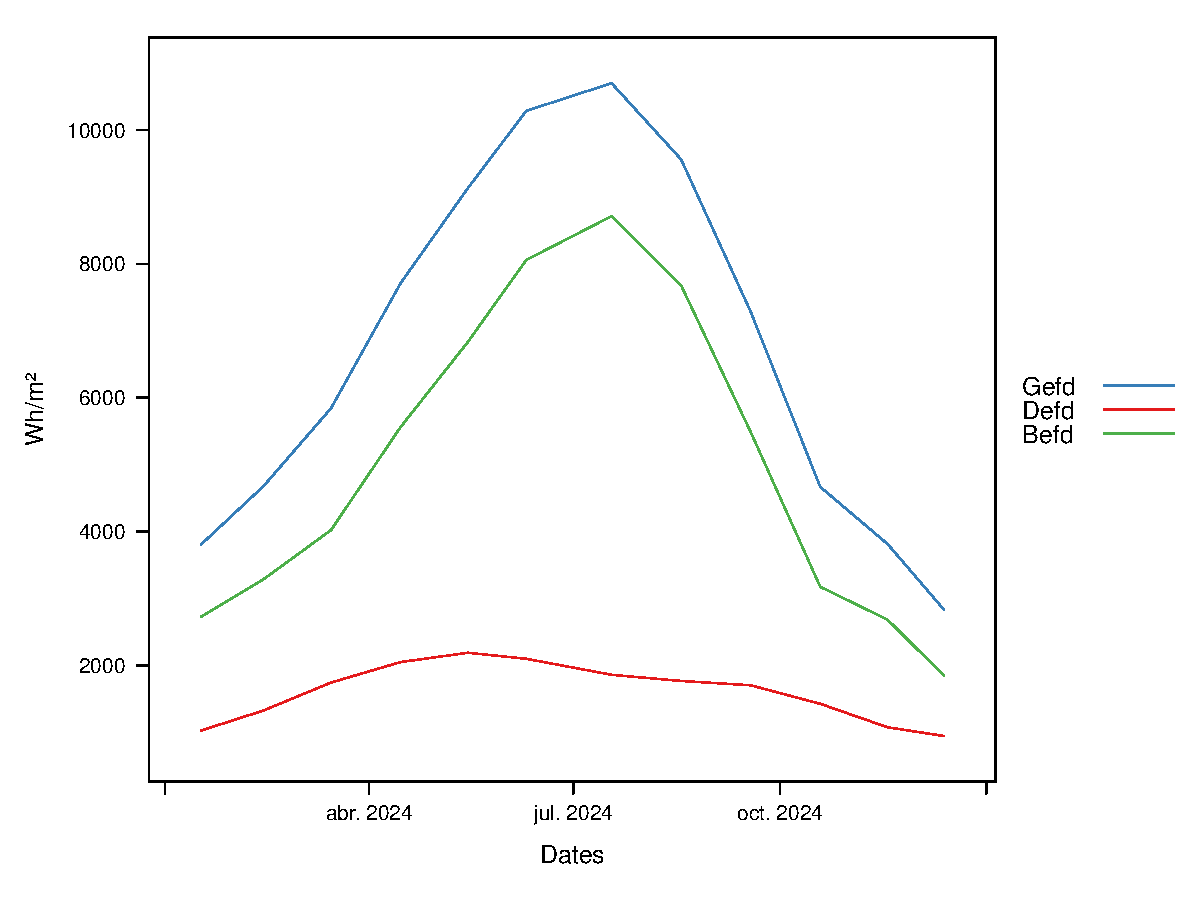
\includegraphics[width=0.8\textwidth]{figuras/codigo-gef.pdf}
\end{center}
\section{Producción eléctrica de un SFCR}
\label{sec:org08954cc}
\label{produccion-electrica-sfcr}
Con la radiación efectiva, se puede estimar la producción eléctrica que va a tener un sistema fotovoltaico conectado a red. Esta estimación, se puede calcular mediante la función \texttt{prodGCPV} la cual mediante la función \texttt{fProd} procesa un objeto de clase \texttt{Gef} y obtiene un objeto \texttt{ProdGCPV}.

Como se puede ver en la figura \ref{fig:prodgcpv}, \texttt{prodGCPV} funciona gracias a la siguiente función:
\begin{figure}[htbp]
\centering
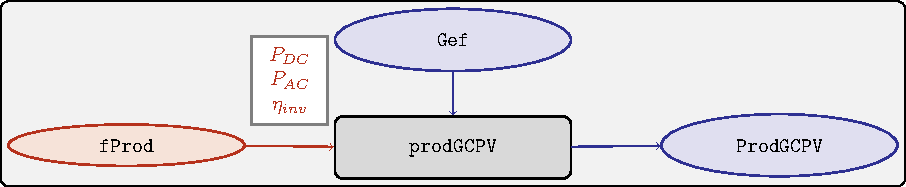
\includegraphics[keepaspectratio,width=0.8\textwidth,height=\textheight]{figuras/prodgcpv.pdf}
\caption{Estimación de la producción eléctrica de un SFCR mediante la función \texttt{prodGCPV}, la cual emplea la función \texttt{fProd} para el computo de la potencia a la entrada (\(P_{DC}\)), a la salida (\(P_{AC}\)) y el rendimiento (\(\eta_{inv}\)) del inversor. \label{fig:prodgcpv}}
\end{figure}
\begin{itemize}
\item \texttt{fProd}: simula el comportamiento de un sistema fotovoltaico conectado a red bajo diferentes condiciones de temperatura e irradiancia. Tiene los siguientes argumentos:
\begin{itemize}
\item \texttt{inclin}: puede ser tanto un objeto de clase \texttt{Gef} como un \texttt{data.frame} (o \texttt{data.table}). Sin embargo, si es un \texttt{data.frame}, debe contener como mínimo una columna para \texttt{Gef} y otra para \texttt{Ta}
\item \texttt{module}: una lista de valores numéricos con la información sobre el módulo fotovoltaico:
\begin{itemize}
\item \texttt{Vocn}: tensión de circuito abierto en STC (\(V_{oc}^*\))(condiciones estandar de médida). Por defecto, tiene un valor de \(57.2V\).
\item \texttt{Iscn}: corriente de cortocircuito en STC (\(I_{sc}^*\)). Por defecto, tiene un valor de \(4.7A\).
\item \texttt{Vmn}: tensión en el punto de máxima potencia en STC (\(I_{MPP}^*\)). Por defecto, tiene un valor de \(46.08V\).
\item \texttt{Imn}: corriente de cortocircuito en STC (\(I_{MPP}^*\)). Por defecto, tiene un valor de \(4.35A\)).
\item \texttt{Ncs}: número de células en serie dentro del módulo. Por defecto, tiene un valor de 96.
\item \texttt{Ncp}: número de células en paralelo dentro del módulo. Por defecto, tiene un valor de 1.
\item \texttt{CoefVT}: coeficiente de disminución de la tensión  de cada célula con la temperatura (\(dV_{oc}/dT_c\)). Por defecto, tiene un valor de \(-0.0023 V/^\circ C\).
\item \texttt{TONC}: temperatura de operación nominal de célula (\(TONC\)). Por defecto, tiene un valor de \(47^\circ C\).
\end{itemize}
\item \texttt{generator}: lista de valores numéricos con la información sobre el generador:
\begin{itemize}
\item \texttt{Nms}: número de módulos en serie. Por defecto, tiene un valor de 12.
\item \texttt{Nmp}: número de módulos en paralelo. Por defecto, tiene un valor de 11.
\end{itemize}
\item \texttt{inverter}: lista de valores númericos con la información del inversor DC/AC.
\begin{itemize}
\item \texttt{Ki}: coeficientes de la curva de eficiencia del inversor. Se puede presentar en un vector de 3 valores (por defecto, \texttt{c(0.01, 0.025, 0.05)}) o una matriz de 9 valores (si tiene dependencia del voltage).
\item \texttt{Pinv}: potencia nominal del inversor. Por defecto, tiene un valor de \(25000 W\).
\item \texttt{Vmin}: mínima tensión del rango MPP del inversor. Por defecto, tiene un valor de \(420V\).
\item \texttt{Vmax}: máxima tensión del rango MPP del inversor. Por defecto, tiene un valor de \(750V\).
\item \texttt{Gumb}: irradiancia umbral de funcionamienot del inversor. Por defecto, tiene un valor de \(20W/m^2\).
\end{itemize}
\item \texttt{effSys}: una lista de valores numéricos con la información sobre las pérdidas del sistema.
\begin{itemize}
\item \texttt{ModQual}: tolerancia media del set de módulos (\(\%\)). Por defecto, tiene un valor de 3.
\item \texttt{ModDisp}: pérdidas por dispersión en los módulos (\(\%\)). Por defecto, tiene un valor de 2.
\item \texttt{OhmDC}: pérdidas por efecto Joule en el cableado de DC (\(\%\)). Por defecto, tiene un valor de 1.5.
\item \texttt{OhmAC}: pérdidas por efecto Joule en el cableado de AC (\(\%\)). Por defecto, tiene un valor de 1.5.
\item \texttt{MPP}: error promedio del algoritmo de búsqueda del MPP del inversor (\(\%\)). Por defecto, tiene un valor de 1.
\item \texttt{TrafoMT}: pérdidas por el transformador MT (\(\%\)). Por defecto, tiene un valor de 1.
\item \texttt{Disp}: pérdidas por las paradas del sistema (\(\%\)). Por defecto, tiene un valor de 0.5.
\end{itemize}
\end{itemize}
\end{itemize}
\begin{lstlisting}[numbers=left,language=r,label= ,caption= ,captionpos=b]
inclin <- calcGef(lat, dataRad = prom, keep.night = FALSE)
module <- list(Vocn=57.6, Iscn=4.7, Vmn=46.08, Imn=4.35,
               Ncs=96, Ncp=1, CoefVT=0.0023, TONC=47)
generator <- list(Nms=12, Nmp=11)
inverter <- list(Ki=c(0.01, 0.025, 0.05), Pinv=25000,
                 Vmin=420, Vmax=750, Gumb=20)
effSys <- list(ModQual=3, ModDisp=2, OhmDC=1.5, OhmAC=1.5,
               MPP=1, TrafoMT=1, Disp=0.5)
prod <- fProd(inclin = inclin, module = module,
              generator = generator, inverter = inverter,
              effSys = effSys)
show(prod)
\end{lstlisting}

\begin{verbatim}
                   Dates       Tc      Voc       Isc     Vmpp      Impp      Vdc       Idc       Pac
                  <POSc>    <num>    <num>     <num>    <num>     <num>    <num>     <num>     <num>
  1: 2024-01-17 08:00:00 15.27689 716.9624  8.083413 607.4640  7.620135 607.4640  7.620135  3796.209
  2: 2024-01-17 09:00:00 21.43284 700.6516 17.513415 583.9663 16.433741 583.9663 16.433741  8053.912
  3: 2024-01-17 10:00:00 27.23609 685.2753 26.403138 562.0190 24.658263 562.0190 24.658263 11650.920
  4: 2024-01-17 11:00:00 31.48724 674.0114 32.915263 546.0746 30.625265 546.0746 30.625265 14041.629
  5: 2024-01-17 12:00:00 33.33104 669.1261 35.739693 539.1958 33.196772 539.1958 33.196772 15016.481
 ---                                                                                                
141: 2024-12-13 12:00:00 33.94967 667.4869 28.721724 542.4718 26.706186 542.4718 26.706186 12177.570
142: 2024-12-13 13:00:00 32.55186 671.1906 26.580476 547.6944 24.746716 547.6944 24.746716 11395.331
143: 2024-12-13 14:00:00 29.08872 680.3665 21.275466 560.6878 19.868077 560.6878 19.868077  9362.088
144: 2024-12-13 15:00:00 24.29331 693.0724 13.929608 578.8034 13.059814 578.8034 13.059814  6316.091
145: 2024-12-13 16:00:00 19.21305 706.5331  6.147403 598.1441  5.786102 598.1441  5.786102  2784.663
           Pdc      EffI
         <num>     <num>
  1:  4290.940 0.9118076
  2:  8895.974 0.9330800
  3: 12846.437 0.9347232
  4: 15502.477 0.9335163
  5: 16592.492 0.9327431
 ---                    
141: 13429.451 0.9345615
142: 12563.918 0.9347755
143: 10326.335 0.9343983
144:  7007.083 0.9290019
145:  3208.198 0.8945754
\end{verbatim}

Esta función brinda estos datos a la función \texttt{prodGCPV} para que produzca un objeto de clase \texttt{ProdGCPV} como resultado. Esta función tiene como argumentos principales los mismo que \texttt{calcGef}, ya que parte de un objeto tipo \texttt{Gef}, y los argumentos de la función \texttt{fProd}.
\begin{lstlisting}[numbers=left,language=r,label= ,caption= ,captionpos=b]
prodFixed <- prodGCPV(lat, modeTrk = 'fixed', dataRad = prom)
show(prodFixed)
\end{lstlisting}

\begin{verbatim}
Object of class  ProdGCPV 

Source of meteorological information: prom- 

Latitude of source:  37.2 degrees
Latitude for calculations:  37.2 degrees

Monthly avarages:
        Dates       Eac       Edc       Yf
       <char>     <num>     <num>    <num>
 1: Jan. 2024  6678.640  6978.809 4.095437
 2: Feb. 2024  7194.835  7519.763 4.411976
 3: Mar. 2024  7843.267  8195.794 4.809603
 4: Apr. 2024  8929.962  9336.190 5.475980
 5: May. 2024  9484.132  9914.605 5.815805
 6: Jun. 2024  9862.108 10309.878 6.047585
 7: Jul. 2024 10019.327 10475.108 6.143994
 8: Aug. 2024  9703.467 10142.955 5.950304
 9: Sep. 2024  8757.170  9151.202 5.370022
10: Oct. 2024  6908.624  7220.274 4.236467
11: Nov. 2024  6431.264  6720.101 3.943743
12: Dec. 2024  5229.190  5463.318 3.206614

Yearly values:
   Dates     Eac     Edc       Yf
   <int>   <num>   <num>    <num>
1:  2024 2959931 3093711 1815.072
-----------------
Mode of tracking:  fixed 
    Inclination:  27.2 
    Orientation:  0 
-----------------
Generator:
    Modules in series:  22 
    Modules in parallel:  130 
    Nominal power (kWp):  1630.8
\end{verbatim}

\begin{lstlisting}[numbers=left,language=r,label= ,caption= ,captionpos=b]
prod2x <- prodGCPV(lat, modeTrk = 'two', dataRad = prom)
show(prod2x)
\end{lstlisting}

\begin{verbatim}
Object of class  ProdGCPV 

Source of meteorological information: prom- 

Latitude of source:  37.2 degrees
Latitude for calculations:  37.2 degrees

Monthly avarages:
        Dates       Eac       Edc       Yf
       <char>     <num>     <num>    <num>
 1: Jan. 2024  9725.125 10159.052 5.963585
 2: Feb. 2024 10163.306 10616.084 6.232284
 3: Mar. 2024 10793.363 11273.933 6.618644
 4: Apr. 2024 12779.088 13349.623 7.836319
 5: May. 2024 14473.608 15121.428 8.875422
 6: Jun. 2024 16252.186 16981.660 9.966072
 7: Jul. 2024 15916.049 16632.343 9.759948
 8: Aug. 2024 14511.287 15163.412 8.898528
 9: Sep. 2024 12350.603 12903.142 7.573565
10: Oct. 2024  9458.655  9878.812 5.800182
11: Nov. 2024  9177.823  9586.046 5.627972
12: Dec. 2024  7284.466  7606.879 4.466938

Yearly values:
   Dates     Eac     Edc       Yf
   <int>   <num>   <num>    <num>
1:  2024 4358566 4553392 2672.735
-----------------
Mode of tracking:  two 
    Inclination limit: 90 
-----------------
Generator:
    Modules in series:  22 
    Modules in parallel:  130 
    Nominal power (kWp):  1630.8
\end{verbatim}

\begin{lstlisting}[numbers=left,language=r,label= ,caption= ,captionpos=b]
prodHoriz <- prodGCPV(lat, modeTrk = 'horiz', dataRad = prom)
xyplot(prodHoriz)
\end{lstlisting}

\begin{center}
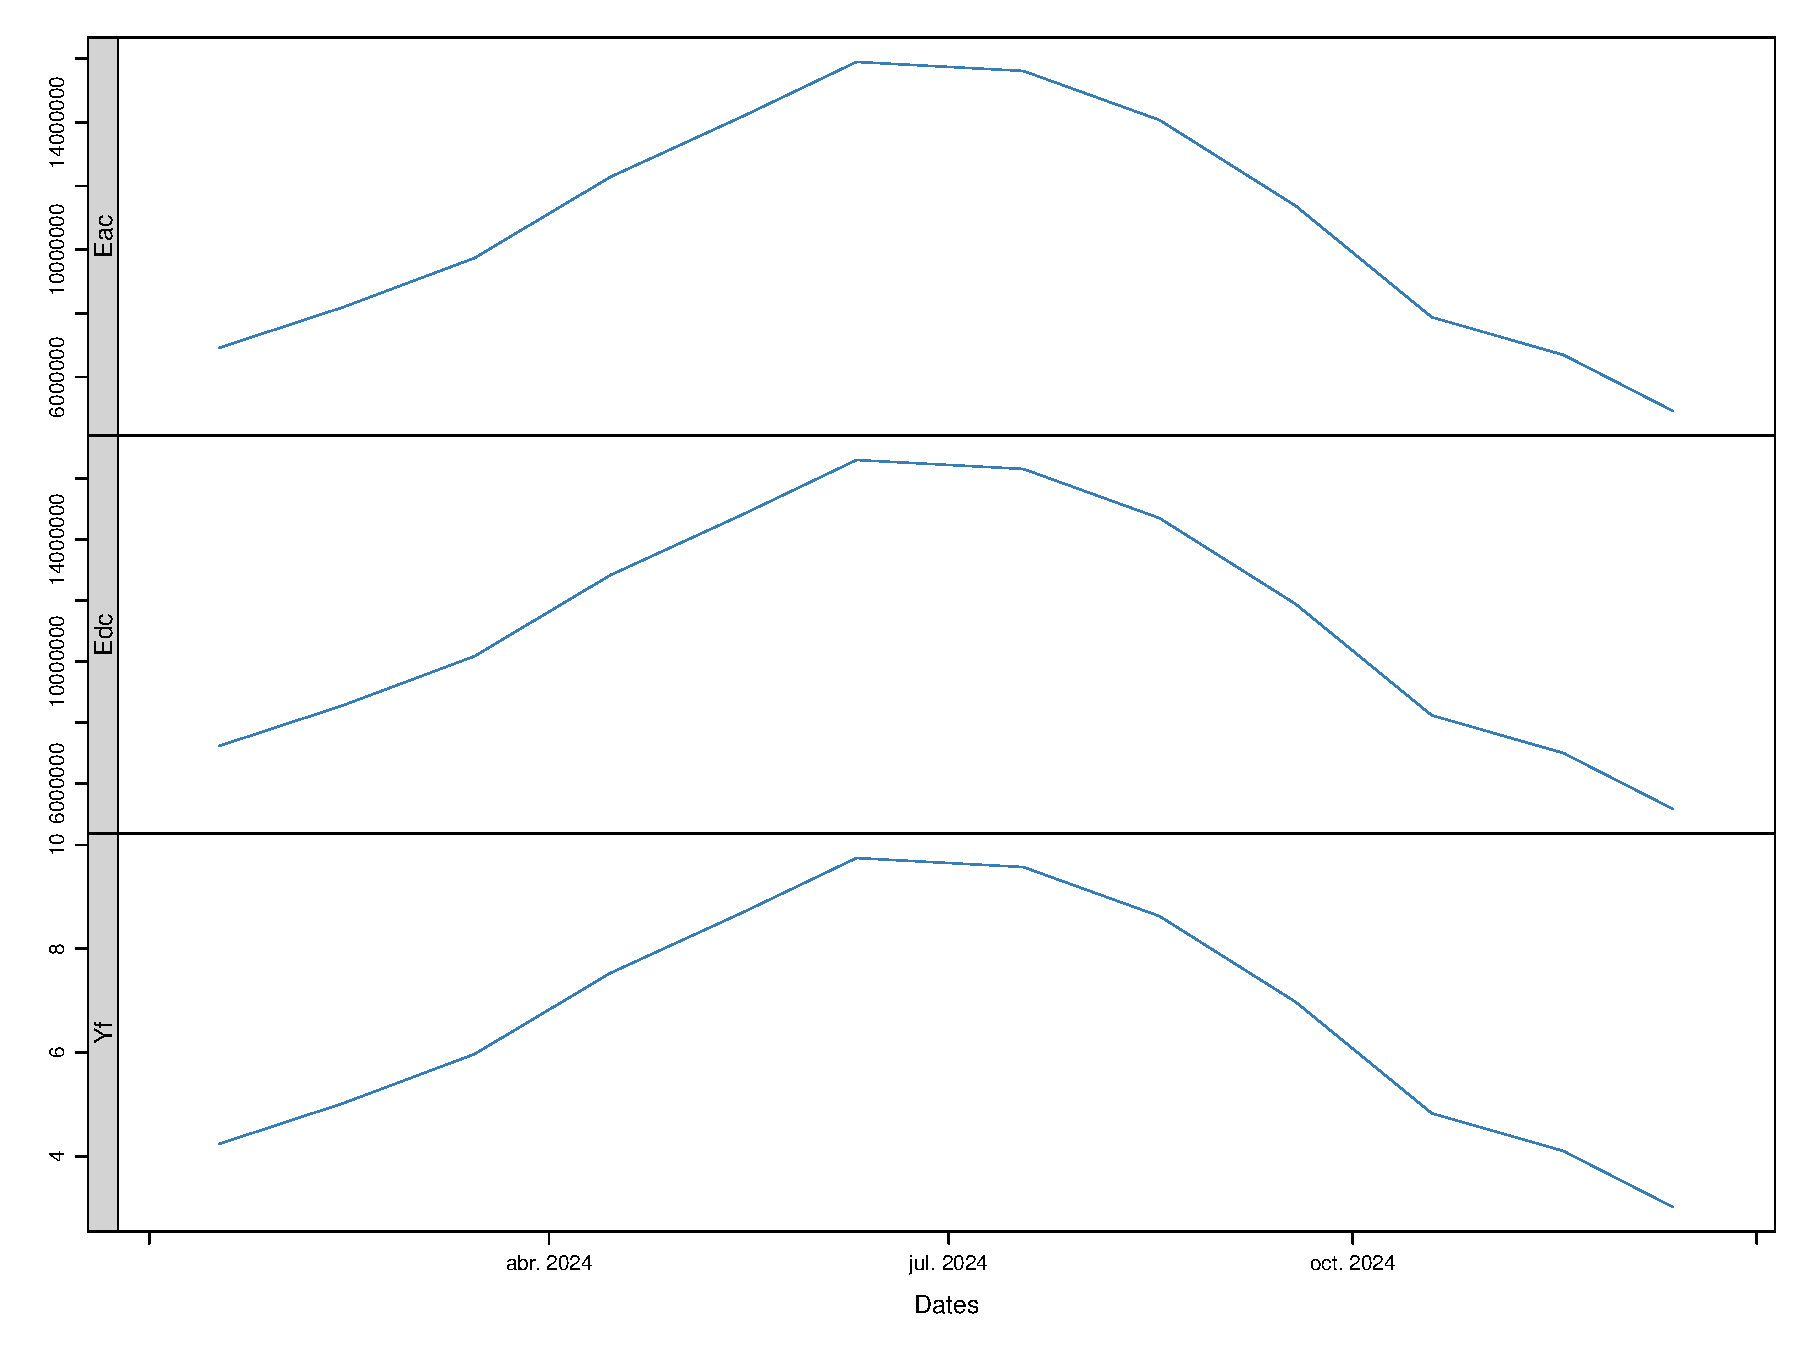
\includegraphics[width=0.8\textwidth]{figuras/codigo-prodgcpv.pdf}
\end{center}

\section{Producción eléctrica de un SFB}
\label{sec:org24597b0}
De igual forma que en el apartado anterior, se puede estimar la producción eléctrica de un sistema fotovoltaico de bombeo.

Como se puede ver en la figura \ref{fig:prodpvps}, \texttt{prodPVPS} funciona gracias a la siguiente función:
\begin{figure}[htbp]
\centering
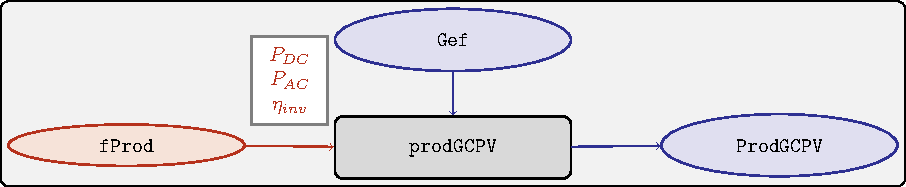
\includegraphics[keepaspectratio,width=0.8\textwidth,height=0.5\textheight]{figuras/prodpvps.pdf}
\caption{Estimación de la producción eléctrica de un SFB mediante la función \texttt{prodPVPS}, la cual emplea la función \texttt{fPump} para el computo del rendimiento de las diferentes parte de una bomba centrífuga alimentada por un convertidor de frecuencia. \label{fig:prodpvps}}
\end{figure}
\begin{itemize}
\item \texttt{fPump}: calcula el rendimiento de las diferentes partes de una bomba centrífuga alimentada por un convertidor de frecuencia siguiendo las leyes de afinidad. Tiene solo dos argumentos:
\begin{itemize}
\item \texttt{pump}: lista que contiene los parametros de la bomba que va a ser simulada. Puede ser una fila de \texttt{pumpCoef}:
\begin{lstlisting}[numbers=left,language=r,label= ,caption= ,captionpos=b]
CoefSP8A44 <- pumpCoef[Qn == 8 & stages == 44]
show(CoefSP8A44)
\end{lstlisting}

\begin{verbatim}
      Qn stages  Qmax   Pmn         a         b      c     g     h     i       j     k      l
   <int>  <int> <num> <int>     <num>     <num>  <num> <num> <num> <num>   <num> <num>  <num>
1:     8     44    12  7500 0.1043011 -0.101288 -0.726 -0.24  0.42  0.64 -0.0058 0.095 0.2013
\end{verbatim}

\item \texttt{H}: el salto manometrico total.
\end{itemize}
\begin{lstlisting}[numbers=left,language=r,label= ,caption= ,captionpos=b]
fSP8A44 <- fPump(pump = CoefSP8A44, H = 40)
\end{lstlisting}

Obtiene como resultado los siguientes valores y funciones:
\begin{itemize}
\item \texttt{lim}: rango de valores de la potencia eléctrica de salida.
\begin{lstlisting}[numbers=left,language=r,label= ,caption= ,captionpos=b]
show(fSP8A44$lim)
\end{lstlisting}

\begin{verbatim}
[1]  190.100 4084.218
\end{verbatim}

\item \texttt{fQ}: función que relaciona el caudal con la potencia eléctrica.
\begin{lstlisting}[numbers=left,language=r,label= ,caption= ,captionpos=b]
show(fSP8A44$fQ)
\end{lstlisting}

\begin{verbatim}
function (x, deriv = 0L) 
{
    deriv <- as.integer(deriv)
    if (deriv < 0L || deriv > 3L) 
	stop("'deriv' must be between 0 and 3")
    if (deriv > 0L) {
	z0 <- double(z$n)
	z[c("y", "b", "c")] <- switch(deriv, list(y = z$b, b = 2 * 
	    z$c, c = 3 * z$d), list(y = 2 * z$c, b = 6 * z$d, 
	    c = z0), list(y = 6 * z$d, b = z0, c = z0))
	z[["d"]] <- z0
    }
    res <- .splinefun(x, z)
    if (deriv > 0 && z$method == 2 && any(ind <- x <= z$x[1L])) 
	res[ind] <- ifelse(deriv == 1, z$y[1L], 0)
    res
}
<bytecode: 0x000002d6fbeb1468>
<environment: 0x000002d6fb151f98>
\end{verbatim}

\item \texttt{fPb}: función que relaciona la potencia del eje de la bomba con la potencia eléctrica del motor.
\begin{lstlisting}[numbers=left,language=r,label= ,caption= ,captionpos=b]
show(fSP8A44$fPb)
\end{lstlisting}

\begin{verbatim}
function (x, deriv = 0L) 
{
    deriv <- as.integer(deriv)
    if (deriv < 0L || deriv > 3L) 
	stop("'deriv' must be between 0 and 3")
    if (deriv > 0L) {
	z0 <- double(z$n)
	z[c("y", "b", "c")] <- switch(deriv, list(y = z$b, b = 2 * 
	    z$c, c = 3 * z$d), list(y = 2 * z$c, b = 6 * z$d, 
	    c = z0), list(y = 6 * z$d, b = z0, c = z0))
	z[["d"]] <- z0
    }
    res <- .splinefun(x, z)
    if (deriv > 0 && z$method == 2 && any(ind <- x <= z$x[1L])) 
	res[ind] <- ifelse(deriv == 1, z$y[1L], 0)
    res
}
<bytecode: 0x000002d6fbeb1468>
<environment: 0x000002d6fb136550>
\end{verbatim}

\item \texttt{fPh}: función que relaciona la potencia hidráulica con la potencia eléctrica del motor.
\begin{lstlisting}[numbers=left,language=r,label= ,caption= ,captionpos=b]
show(fSP8A44$fPh)
\end{lstlisting}

\begin{verbatim}
function (x, deriv = 0L) 
{
    deriv <- as.integer(deriv)
    if (deriv < 0L || deriv > 3L) 
	stop("'deriv' must be between 0 and 3")
    if (deriv > 0L) {
	z0 <- double(z$n)
	z[c("y", "b", "c")] <- switch(deriv, list(y = z$b, b = 2 * 
	    z$c, c = 3 * z$d), list(y = 2 * z$c, b = 6 * z$d, 
	    c = z0), list(y = 6 * z$d, b = z0, c = z0))
	z[["d"]] <- z0
    }
    res <- .splinefun(x, z)
    if (deriv > 0 && z$method == 2 && any(ind <- x <= z$x[1L])) 
	res[ind] <- ifelse(deriv == 1, z$y[1L], 0)
    res
}
<bytecode: 0x000002d6fbeb1468>
<environment: 0x000002d6fb1315b8>
\end{verbatim}

\item \texttt{fFreq}: función que relaciona la frecuencia con la potencia eléctrica del motor.
\begin{lstlisting}[numbers=left,language=r,label= ,caption= ,captionpos=b]
show(fSP8A44$fFreq)
\end{lstlisting}

\begin{verbatim}
function (x, deriv = 0L) 
{
    deriv <- as.integer(deriv)
    if (deriv < 0L || deriv > 3L) 
	stop("'deriv' must be between 0 and 3")
    if (deriv > 0L) {
	z0 <- double(z$n)
	z[c("y", "b", "c")] <- switch(deriv, list(y = z$b, b = 2 * 
	    z$c, c = 3 * z$d), list(y = 2 * z$c, b = 6 * z$d, 
	    c = z0), list(y = 6 * z$d, b = z0, c = z0))
	z[["d"]] <- z0
    }
    res <- .splinefun(x, z)
    if (deriv > 0 && z$method == 2 && any(ind <- x <= z$x[1L])) 
	res[ind] <- ifelse(deriv == 1, z$y[1L], 0)
    res
}
<bytecode: 0x000002d6fbeb1468>
<environment: 0x000002d6fb150d60>
\end{verbatim}
\end{itemize}

Se pueden realizar operaciones con este objeto:
\begin{lstlisting}[numbers=left,language=r,label= ,caption= ,captionpos=b]
SP8A44 = with(fSP8A44,{
  Pac = seq(lim[1],lim[2],l=10)
  Pb = fPb(Pac)
  etam = Pb/Pac
  Ph = fPh(Pac)
  etab = Ph/Pb
  f = fFreq(Pac)
  Q = fQ(Pac)
  result = data.table(Q,Pac,Pb,Ph,etam,etab,f)})
show(SP8A44)
\end{lstlisting}

\begin{verbatim}
	     Q       Pac        Pb         Ph      etam      etab        f
	 <num>     <num>     <num>      <num>     <num>     <num>    <num>
 1:  0.3133325  190.1000  124.8346   34.15325 0.6566786 0.2735880 20.47033
 2:  2.0718468  622.7798  429.6728  225.83130 0.6899274 0.5255890 22.33036
 3:  4.0764128 1055.4595  752.8970  444.32900 0.7133358 0.5901591 25.51459
 4:  5.6406747 1488.1393 1087.3665  614.83354 0.7306887 0.5654336 28.73213
 5:  6.9474993 1920.8190 1429.7984  757.27743 0.7443692 0.5296393 31.78514
 6:  8.1028841 2353.4988 1778.0156  883.21437 0.7554776 0.4967416 34.69527
 7:  9.1607296 2786.1786 2130.4683  998.51953 0.7646560 0.4686855 37.49608
 8: 10.1514390 3218.8583 2486.0213 1106.50685 0.7723301 0.4450915 40.21428
 9: 11.0937480 3651.5381 2843.8295 1209.21854 0.7788032 0.4252078 42.86977
10: 12.0000000 4084.2179 3203.2578 1308.00000 0.7843014 0.4083343 45.47737
\end{verbatim}

Está función entrega todos estos resultados a \texttt{prodPVPS} la cual calcula los resultados en base a la potencia del generador a simular, y devuleve un objeto de clase \texttt{ProdPVPS}.
\begin{lstlisting}[numbers=left,language=r,label= ,caption= ,captionpos=b]
prodsfb <- prodPVPS(lat, modeTrk = 'fixed', dataRad = prom,
                    pump = CoefSP8A44, H = 40, Pg = SP8A44$Pac[10])
xyplot(prodsfb)
\end{lstlisting}

\begin{center}
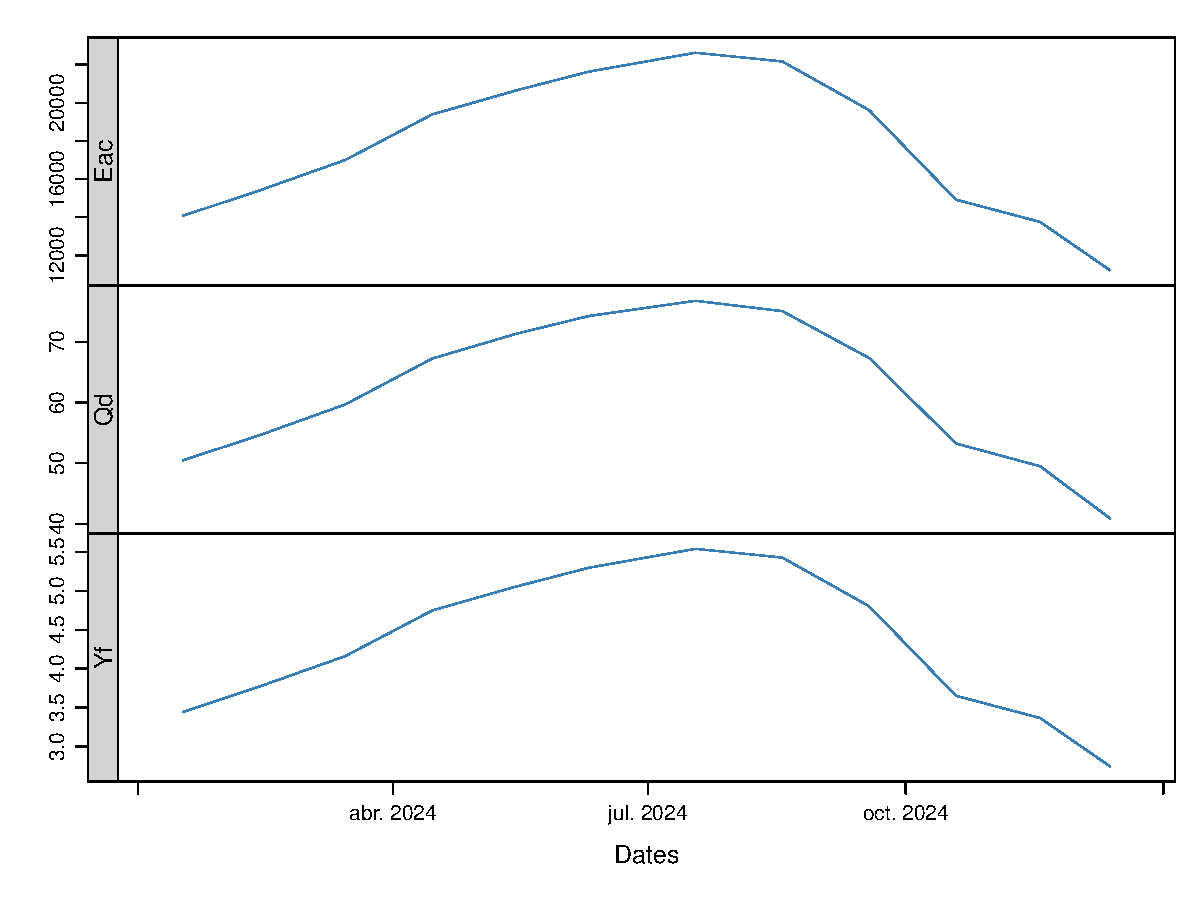
\includegraphics[width=0.8\textwidth]{figuras/codigo-prodpvps.pdf}
\end{center}
\end{itemize}
\section{Optimización de distancias}
\label{sec:orgd5f1334}
\label{optimizacion-distancias}
Por último, el paquete \texttt{solaR2} contiene una función que permite calcular un conjunto de combinaciones de distancias entre los elementos de un sistema fotovoltaico conectado a red, con el fin de que el usuario posteriormente pueda optar cual es la opción mas rentable en base a los precios del cableado y de la ocupación del terreno.

Esta función es \texttt{optimShd}, la cual en base a una resolución (determinada por el argumento \texttt{res}, el cual, indica el incremento de la secuencia de distancias) obtiene la producción de cada combinación y la plasma en un objeto de clase \texttt{Shade}.
\begin{lstlisting}[numbers=left,language=r,label= ,caption= ,captionpos=b]
struct2x <- list(W = 23.11, L = 9.8, Nrow = 2, Ncol = 3)
dist2x <- list(Lew = c(30, 45), Lns = c(20, 40))
ShdM2x <- optimShd(lat, dataRad = prom, modeTrk = 'two',
                   modeShd = c('area', 'prom'),
                   distances = dist2x, struct = struct2x,
                   res = 5,
                   prog = FALSE) #Se quita la barra de progreso
shadeplot(ShdM2x)
\end{lstlisting}

\begin{center}
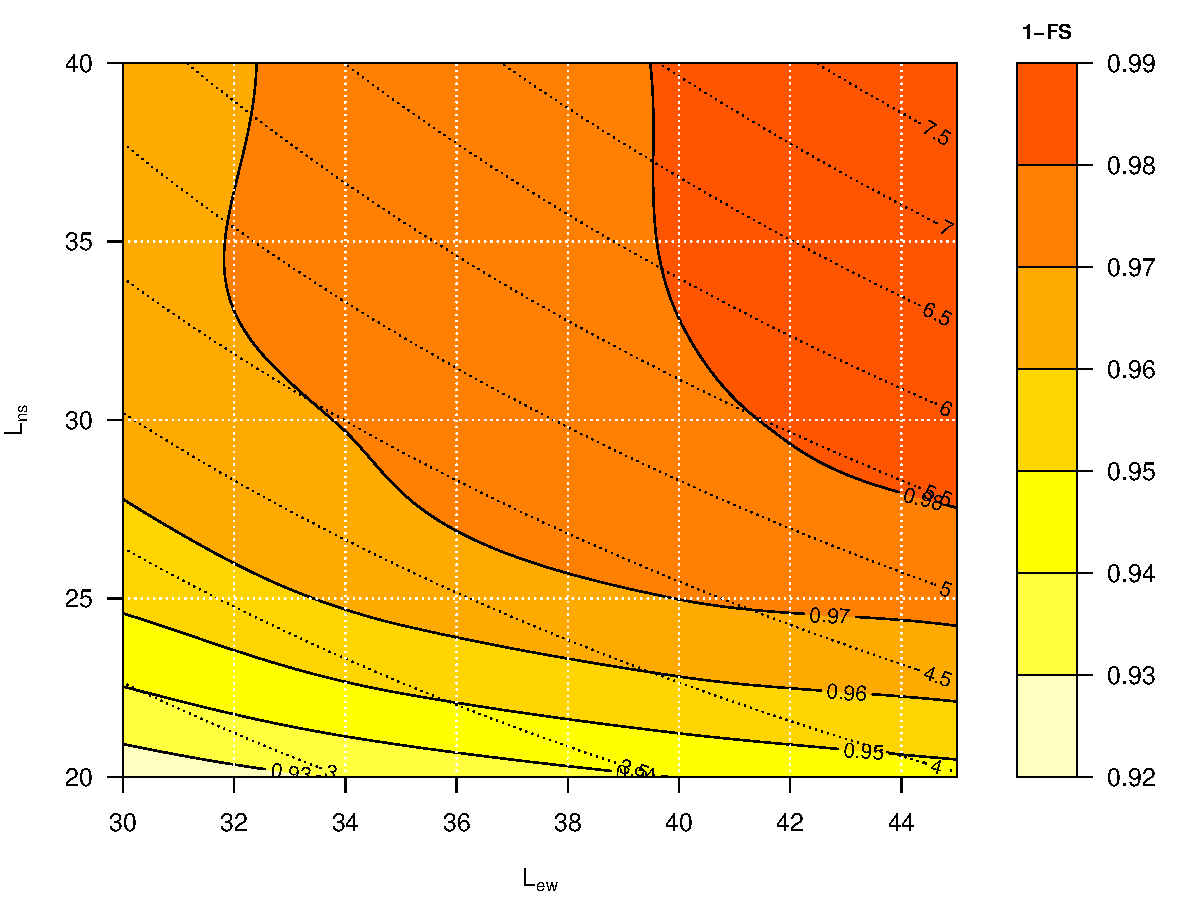
\includegraphics[width=0.8\textwidth]{figuras/codigo-optimshd2x.pdf}
\end{center}
\begin{lstlisting}[numbers=left,language=r,label= ,caption= ,captionpos=b]
structHoriz = list(L = 4.83)
distHoriz = list(Lew = structHoriz$L * c(2,5))
Shd12HorizBT <- optimShd(lat = lat, dataRad = prom,
                         modeTrk = 'horiz',
                         betaLim = 60,
                         distances = distHoriz, res = 2,
                         struct = structHoriz,
                         modeShd = 'bt',
                         prog = FALSE) #Se quita la barra de progreso
show(Shd12HorizBT)
\end{lstlisting}

\begin{verbatim}
Object of class  Shade 

Source of meteorological information: prom- 

Latitude of source:  37.2 degrees
Latitude for calculations:  37.2 degrees

Monthly avarages:
Dimensions of structure:
$L
[1] 4.83

Shade calculation mode:
[1] "bt"
Productivity without shadows:
Object of class  ProdGCPV 

Source of meteorological information: prom- 

Latitude of source:  37.2 degrees
Latitude for calculations:  37.2 degrees

Monthly avarages:
        Dates       Eac       Edc       Yf
       <char>     <num>     <num>    <num>
 1: Jan. 2024  6789.039  7088.612 4.163135
 2: Feb. 2024  8054.032  8409.761 4.938847
 3: Mar. 2024  9614.838 10040.667 5.895956
 4: Apr. 2024 12160.009 12701.260 7.456691
 5: May. 2024 14028.543 14655.892 8.602502
 6: Jun. 2024 15691.671 16395.713 9.622356
 7: Jul. 2024 15451.474 16145.991 9.475064
 8: Aug. 2024 13931.234 14555.274 8.542831
 9: Sep. 2024 11241.111 11740.699 6.893209
10: Oct. 2024  7780.058  8123.781 4.770842
11: Nov. 2024  6583.802  6874.444 4.037281
12: Dec. 2024  4875.306  5091.940 2.989607

Yearly values:
   Dates     Eac     Edc       Yf
   <int>   <num>   <num>    <num>
1:  2024 3850450 4022013 2361.151
-----------------
Mode of tracking:  horiz 
    Inclination limit: 60 
-----------------
Generator:
    Modules in series:  22 
    Modules in parallel:  130 
    Nominal power (kWp):  1630.8 

Summary of results:
      Lew              H           FS               GRR              Yf      
 Min.   : 9.66   Min.   :0   Min.   :0.04702   Min.   :2.000   Min.   :2036  
 1st Qu.:13.16   1st Qu.:0   1st Qu.:0.05607   1st Qu.:2.725   1st Qu.:2139  
 Median :16.66   Median :0   Median :0.07152   Median :3.449   Median :2192  
 Mean   :16.66   Mean   :0   Mean   :0.07933   Mean   :3.449   Mean   :2174  
 3rd Qu.:20.16   3rd Qu.:0   3rd Qu.:0.09424   3rd Qu.:4.174   3rd Qu.:2229  
 Max.   :23.66   Max.   :0   Max.   :0.13783   Max.   :4.899   Max.   :2250
\end{verbatim}

\begin{lstlisting}[numbers=left,language=r,label= ,caption= ,captionpos=b]
structFixed = list(L = 5)
distFixed = list(D = structFixed$L*c(1,3))
Shd12Fixed <- optimShd(lat = lat, dataRad = prom,
                       modeTrk = 'fixed',
                       distances = distFixed, res = 2,
                       struct = structFixed,
                       modeShd = 'area',
                       prog = FALSE) #Se quita la barra de progreso
shadeplot(Shd12Fixed)
\end{lstlisting}

\begin{center}
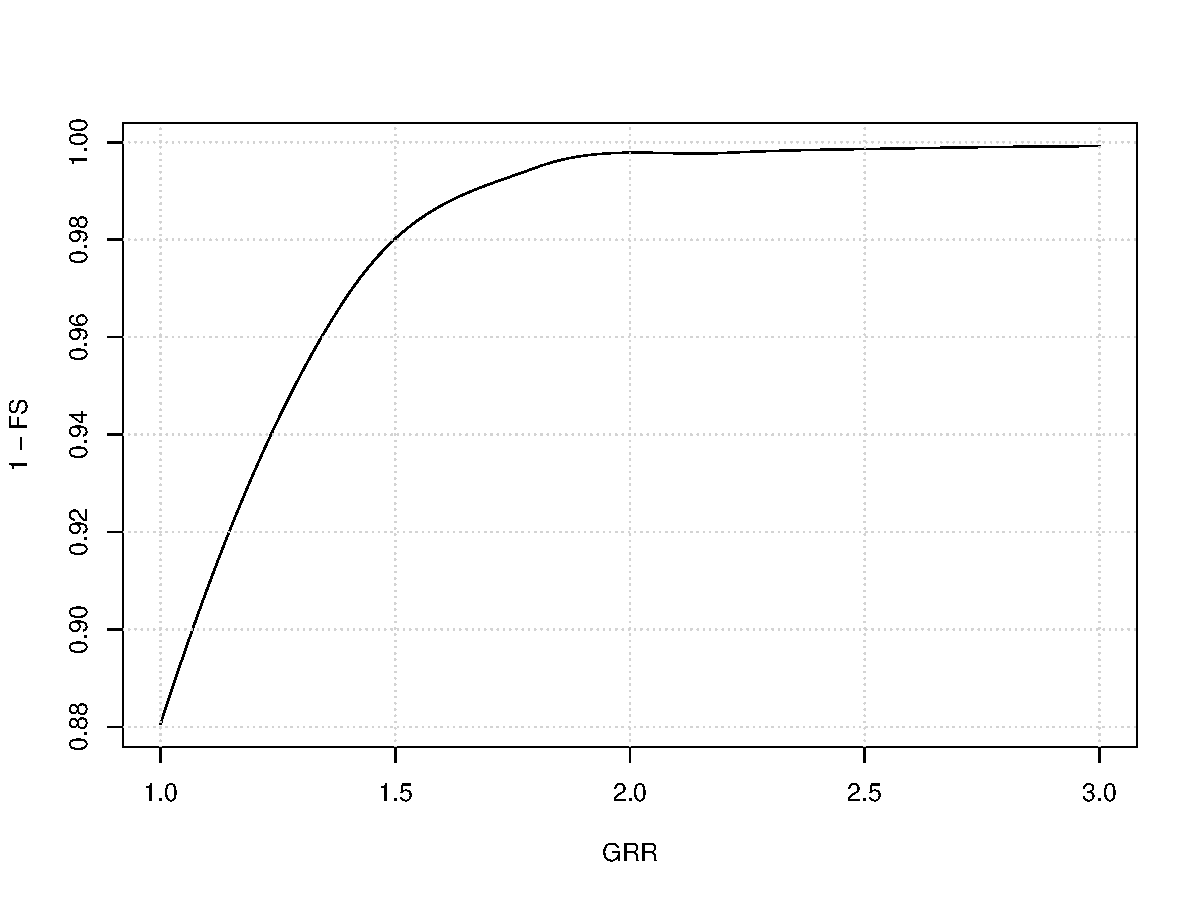
\includegraphics[width=0.8\textwidth]{figuras/codigo-optimshdfixed.pdf}
\end{center}


\section{Aspectos técnicos de la elaboración de un paquete en R}
\label{sec:orgf07702d}
\label{sec:aspectos-tecnicos}
\subsection{Estructura básica del paquete}
\label{sec:org37ba668}
\label{subsec:estructura-paquete}
En la creación de un paquete en \texttt{R}, la estructura de los archivos es clave para asegurar un desarrollo organizado y que \texttt{R} pueda interactuar correctamente con el código y  los datos. Los paquetes de R son esencialmente un conjunto de archivos organizados en un directorio específio. El contenido mínimo requerido incluye:
\begin{itemize}
\item Un archivo \textbf{DESCRIPTION}, que proporciona la información esencial del paquete.
\item Un archivo \textbf{NAMESPACE}, que controla qué funciones y objetos son visibles fuera del paquete.
\item Subdirectoriso como \texttt{R/} y \texttt{man/}:
\begin{itemize}
\item \texttt{R/}: Contiene los archivos de codigo \texttt{.R}, que son las funciones, clases y métodos definidos en el paquete.
\item \texttt{man/}: Contiene las páginas de ayuda y documentación para las funciones, métodos y clases del paqeute.
\end{itemize}
\end{itemize}

La estructura básica de un paquete puede generarse fácilmente utilizando la función \texttt{package.skeleton()}, que crea los archivos y carpetas necesarios para empezar a trabajar en el desarrollo.

\subsection{DESCRIPTION}
\label{sec:org6387016}
\label{subsec:description}
El fichero \textbf{DESCRIPTION} es fundamental, ya que incluye la información descriptiva y técnica del paquete, como el nombre, la versión, los autores y las dependencias. Un ejemplo típico de este archivo es el siguiente:
\begin{examplebox}
\begin{verbatim}
Package: pkgname
Version: 0.5-1
Date: 2004-01-01
Title: My First Collection of Functions
Authors@R: c(person("Joe", "Developer", role = c("aut", "cre"),
                     email = "Joe.Developer@some.domain.net"),
              person("Pat", "Developer", role = "aut"),
              person("A.", "User", role = "ctb",
     	        email = "A.User@whereever.net"))
Author: Joe Developer and Pat Developer, with contributions from A. User
Maintainer: Joe Developer <Joe.Developer@some.domain.net>
Depends: R (>= 1.8.0), nlme
Suggests: MASS
Description: A short (one paragraph) description of what
  the package does and why it may be useful.
License: GPL (>= 2)
URL: http://www.r-project.org, http://www.another.url
\end{verbatim}
\end{examplebox}
Los campos principales de este archivo son:
\begin{itemize}
\item \textbf{Package}: Nombre del paquete.
\item \textbf{Version}: Versión del paquete. Generalmente sigue un esquema de numeración semántica (\texttt{major.minor-patch})\footnote{Un esquema de numeración semántica es un sistema de versiones que sigue un patrón específico para asignar números a las versiones de software. Se utiliza para indicar claramente la magnitud de los cambios realizados y su impacto en la compatibilidad.  Una versión \texttt{major} o mayor se refiere a modificaciones grandes o incompatibles con versiones anteriores, \texttt{minor} o menor es una versión que incluye mejoras o nuevas funciones compatibles con versiones anteriores y \texttt{patch} o parche es una versión que incluye correcciones menores o mejoras que no afectan a la funcionalidad.}.
\item \textbf{Title}: Un título breve pero descriptivo de lo que hace el paquete.
\item \textbf{Authors@R}: Especifica el o los autores con sus respectivos roles, como ``aut'' (autor) y ``cre'' (creador principal).
\item \textbf{Maintainer}: Persona responsable del mantenimiento del paquete, con su correo electrónico.
\item \textbf{Depends}: Lista de dependencias, es decir, otros paquetes de los que depende el correcto funcionamiento del paquete.
\item \textbf{Suggests}: Lista de paqeute que no son obligatorios, pero que pueden ser útiles.
\item \textbf{Description}: Una breve descripción del propósito del paquete.
\item \textbf{License:} Tipo de licencia bajo la cual se distribuye el paquete (GPL, MIT, etc.).
\end{itemize}

Este archivo es crucial para que los usuarios y el sistema \texttt{R} identifiquen las características y requisitos del paquete
\subsection{NAMESPACE}
\label{sec:org3f06ff6}
\label{subsec:namespace}
El archivo \textbf{NAMESPACE} es el encargado de gestionar el espacio de nombres del paquete, permitiendo definir qué funciones y objetos serán visibles (exportados) y cuáles se mantendrán internos. Además, es útil para definir qué funciones o métodos de otros paquetes serán importados para us uso dentro del paquete.

\texttt{R} usa un sistema de gestión de \textbf{espacio de nombres} que permite al autor del paquete especificar:
\begin{itemize}
\item Las \textbf{variables} del paquete que se \textbf{exportan} (y son, por tanto, accesibles a los usuarios).
\item Las \textbf{variables} que se \textbf{importan} de otros paquetes.
\item Las \textbf{clases y métodos} \texttt{S3} y \texttt{S4} que deben registrarse.
\end{itemize}

El \texttt{NAMESPACE} controla la estrategia de búsqueda de variables que utilizan las funciones del paquete:
\begin{itemize}
\item En primer lugar, busca entre las creadas localmente (por el código de la carpeta \texttt{R/}).
\item En segundo lugar, busca entre las variables importadas explícitamente de otros paquetes.
\item En tercer lugar, busca en el \texttt{NAMESPACE} del paquete \texttt{base}.
\item Por último, busca siguiendo el camino habitual (usando \texttt{search()}).
\end{itemize}
\begin{lstlisting}[numbers=left,language=r,label= ,caption= ,captionpos=b]
search()
\end{lstlisting}

\begin{verbatim}
 [1] ".GlobalEnv"           "package:jsonlite"     "package:httr2"        "package:zoo"         
 [5] "package:solaR2"       "package:latticeExtra" "package:lattice"      "package:data.table"  
 [9] "ESSR"                 "package:stats"        "package:graphics"     "package:grDevices"   
[13] "package:utils"        "package:datasets"     "package:methods"      "Autoloads"           
[17] "package:base"
\end{verbatim}

\subsubsection{Manejo de variables}
\label{sec:org528e86a}
\begin{itemize}
\item Exportar variables:
\begin{lstlisting}[numbers=left,language=r,label= ,caption= ,captionpos=b]
export(f, g)
\end{lstlisting}
Esto asegura que las variables \texttt{f} y \texttt{g} sean accesibles desde fuera del paquete.
\item Importar \textbf{todas} las variables de otro paquete:
\begin{lstlisting}[numbers=left,language=r,label= ,caption= ,captionpos=b]
import(pkgExt)
\end{lstlisting}
\item Importar variables \textbf{concretas} de otro paquete:
\begin{lstlisting}[numbers=left,language=r,label= ,caption= ,captionpos=b]
importFrom(pkgExt, var1, var2)
\end{lstlisting}
\end{itemize}
\subsubsection{Manejo de clases y métodos}
\label{sec:org951e5fd}
\begin{itemize}
\item Para registrar un \textbf{método} para una \textbf{clase} determinada:
\begin{lstlisting}[numbers=left,language=r,label= ,caption= ,captionpos=b]
S3method(print, myClass)
\end{lstlisting}
Esto permite definir cómo se imprimen objetos de la clase \texttt{myClass}
\item Para los paquetes que utilizan clases y métodos \texttt{S4}, es necesario agregar una dependencia explícita en el archivo \textbf{DESCRIPTION}:
\end{itemize}
\begin{lstlisting}[numbers=left,language=r,label= ,caption= ,captionpos=b]
import("methods")
\end{lstlisting}
\begin{itemize}
\item Para registrar clases \texttt{S4}:
\end{itemize}
\begin{lstlisting}[numbers=left,language=r,label= ,caption= ,captionpos=b]
exportClasses(class1, class2)
\end{lstlisting}
\begin{itemize}
\item Para registrar métodos \texttt{S4}:
\end{itemize}
\begin{lstlisting}[numbers=left,language=r,label= ,caption= ,captionpos=b]
exportMethods(method1, method2)
\end{lstlisting}
\begin{itemize}
\item Para importar métodos y clases \texttt{S4} de otro paquete:
\end{itemize}
\begin{lstlisting}[numbers=left,language=r,label= ,caption= ,captionpos=b]
importClassesFrom(package, ...)
importMethodsFrom(package, ...)
\end{lstlisting}
\subsection{Documentación}
\label{sec:org320d332}
\label{subsec:documentacion}
La documentación en R sigue un formato específico llamado \texttt{Rd} (\emph{R documentation}), que está inspirado en LaTex. Cada función, método o clase del paquete debe tener una página de documentación asociada, que generalmente se encuentra en el subdirectorio \texttt{man/}. Estas páginas incluyen información sobre el uso de la función, argumentos, detalles de la implementación y ejemplos de uso.
\begin{examplebox}
\begin{verbatim}
\name{load}
\alias{load}
\title{Reload Saved Datasets}
\description{
  Reload the datasets written to a file with the function
  \code{save}.
}
\usage{
  load(file, envir = parent.frame())
}
\arguments{
\item{file}{a connection or a character string giving the
    name of the file to load.}
\item{envir}{the environment where the data should be
    loaded.}
}
\seealso{
  \code{\link{save}}.
}
\examples{
  ## save all data
  save(list = ls(), file= "all.RData")

  ## restore the saved values to the current environment
  load("all.RData")

  ## restore the saved values to the workspace
  load("all.RData", .GlobalEnv)
}
\keyword{file}
\end{verbatim}
\end{examplebox}

El formato tiene varios componentes:
\begin{itemize}
\item \textbf{name}: El nombre de la función.
\item \textbf{alias}: Nombres alternativos o alias de la función.
\item \textbf{title}: Título breve que describe la función.
\item \textbf{description}: Una descripción de lo que hace la función.
\item \textbf{usage}: La sintaxis de la función de lo que hace la función.
\item \textbf{arguments}: Explicación de los argumentos que recibe la función.
\item \textbf{seealso}: Enlaces a funciones relacionadas.
\item \textbf{examples}: Ejemplos de cómo utilizar la función.
\end{itemize}

Esta estructura de documentación permite a los usuarios comprender rápidamente cómo utilizar las funciones del paquete y verificar su funcionalidad con ejemplos prácticos.
